%!TEX root = ../prace.tex

\chapter{Uživatelská dokumentace}

Tato část obsahuje informace o~tom, jak hru spustit a~jaké jsou požadavky ke spuštění. Dále jsou zde uvedeny obrázky ze hry a~popis toho, co znamenají. 

\section{Požadavky pro spuštění hry}
\subsubsection{Hardwarové požadavky}

Doporučená minimální sestava (na ní byla hra vyvíjena): 

\begin{center}
	\begin{tabular} { | l | l |}
		\hline
		Procesor: 	&	Intel i7-2630QM @ 2.00GHz \\	\hline
		RAM:		&	12 GB	(8 GB by mělo také stačit) \\	\hline
		Grafika:	&	ATI Radeon HD 6700M \\	\hline
		OS:			&	Win 10 x64	(7 a~vyšší by měly být v~pohodě) \\
		\hline
	\end{tabular}
\end{center}

Výše uvedneou konfiguraci je potřeba brát jako orientační. Hru jsme úspěšně spustili i~na notebooku s~procesorem Intel i5, integrovanou grafickou kartou a~8 GB operační paměti. Bylo však nutné nastavit grafické vlastnosti na minimální možnou konfiguraci. 

\subsubsection{Softwarové požadavky}

Pro spuštění zkompilované hry není potřeba nic speciálního. Je zapotřebí mít stroj s~minimální uvedenou konfigurací. Dále je dobré mít nainstalované poslední verze ovladačů HW komponent (hlavně grafiky).
Taktéž je zapotřebí mít nainstalovanou poslední verzi DirectX. 


%// TODO povolit obrázky

TODO zmínit tutoriál, jak se k~němu člověk dostane.

%%!TEX root = ../../prace.tex

\section{Hlavní menu}

Po načtení hry hráč vidí hlavní menu. Denní doba i~počasí se zvolí náhodně.

\begin{figure}[!ht]\centering
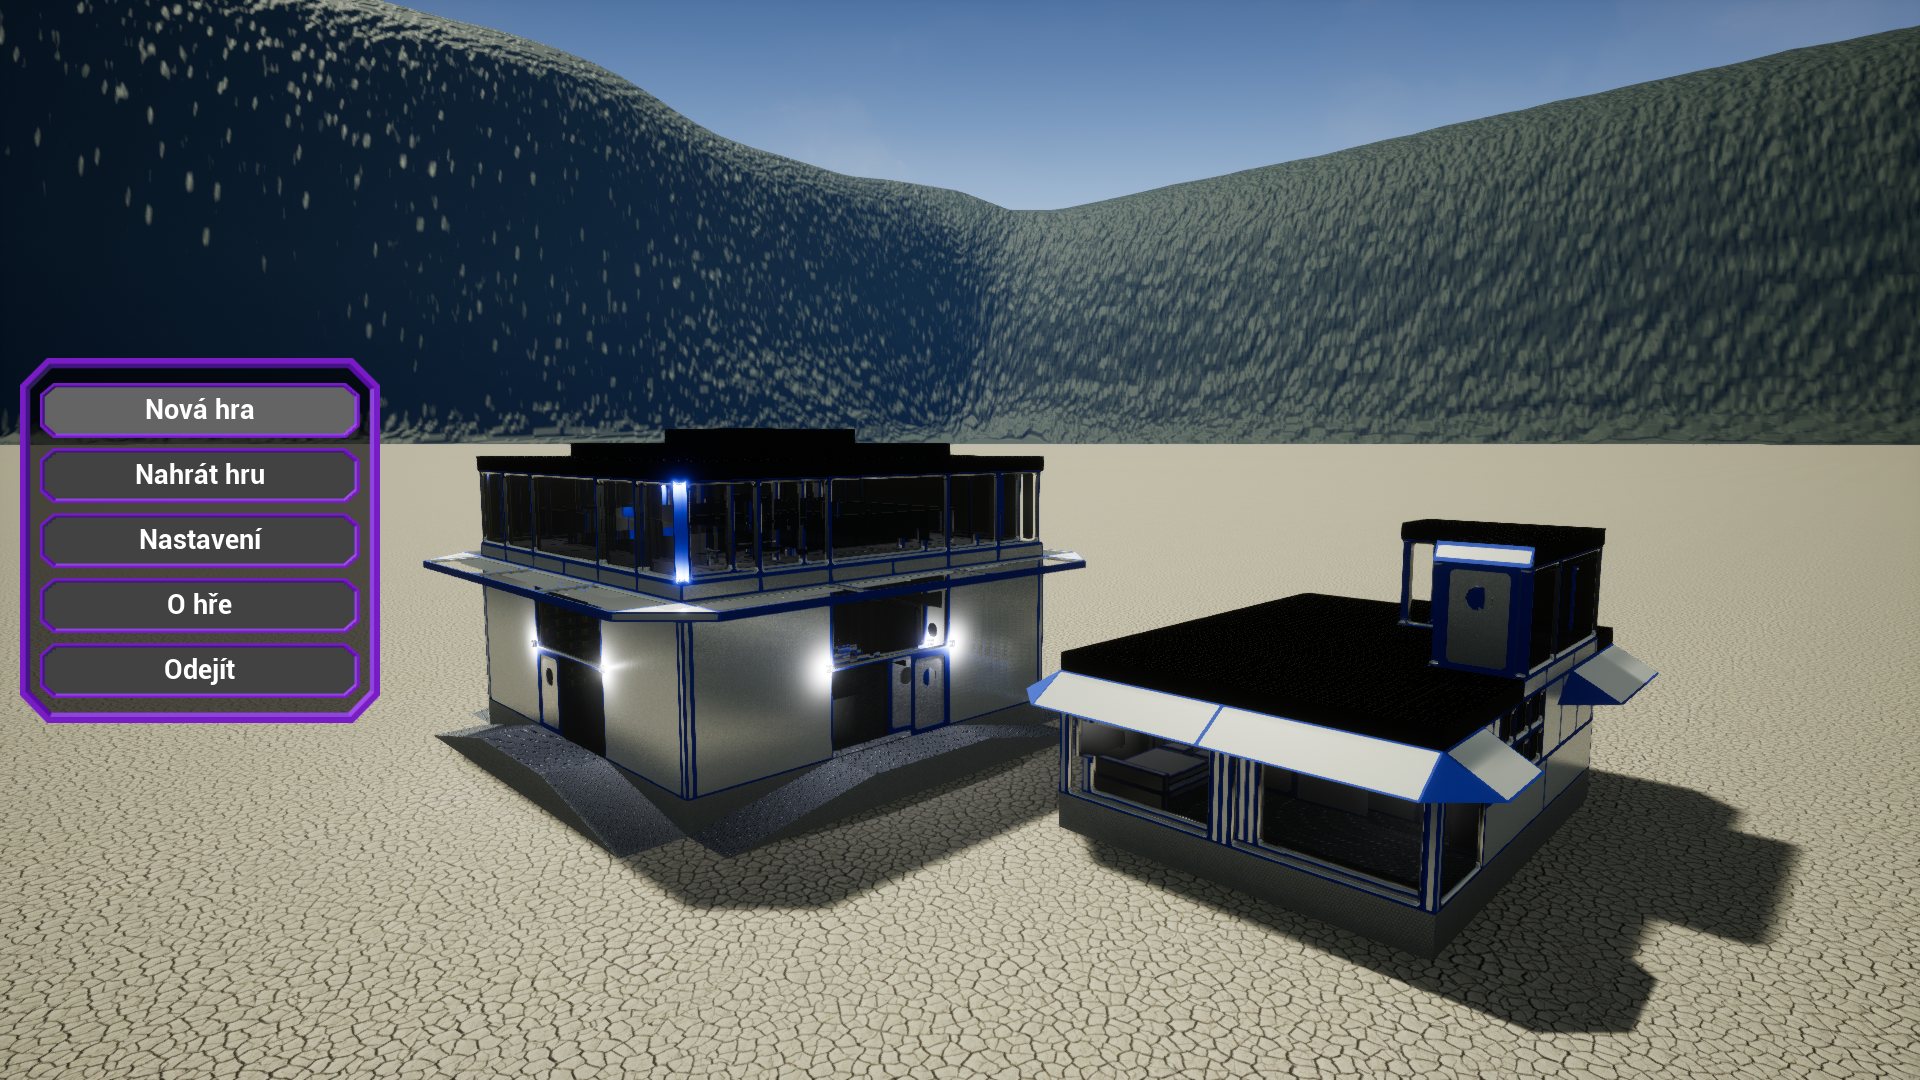
\includegraphics[ width=140mm]{../img/user/mainMenu/mmDay}

\caption{Obrazovka hlavního menu -- den}
\label{fig:user_mainMenu_mmDay}

\end{figure}


\FloatBarrier

První volba, kterou je možné zvolit, je výběr nové hry. K~dispozici je několik variant s~různými obtížnostmi.

\begin{figure}[!ht]\centering
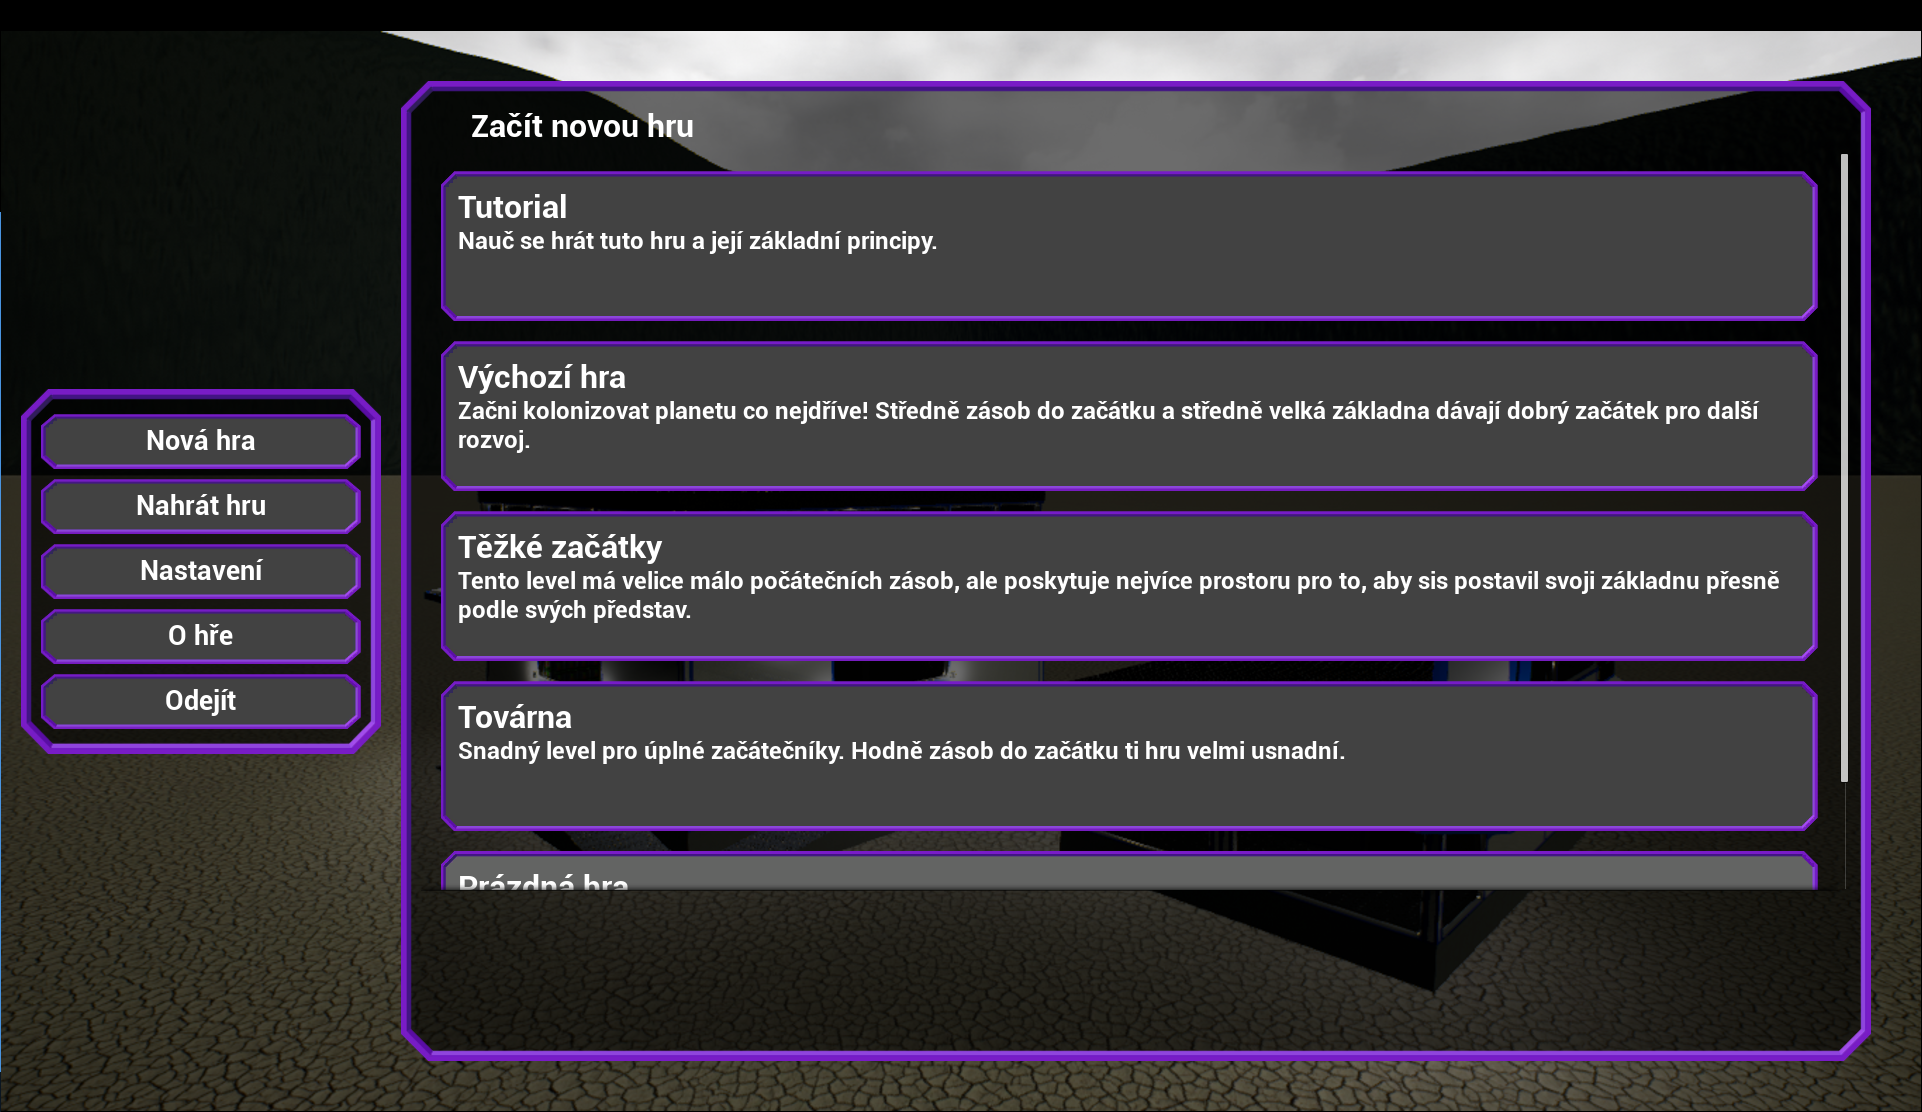
\includegraphics[ width=140mm]{../img/user/mainMenu/mmBegin}

\caption{Obrazovka hlavního menu -- Nová hra}
\label{fig:user_mainMenu_mmBegin}

\end{figure}
\FloatBarrier

Pokud hráč má nějaké uložené hry, může si je nahrát kliknutím na tlačítko \textbf{Nahrát hru}. V~tomto případě žádné uložené hry k~načtení k~dispozici nejsou.

\begin{figure}[!ht]\centering
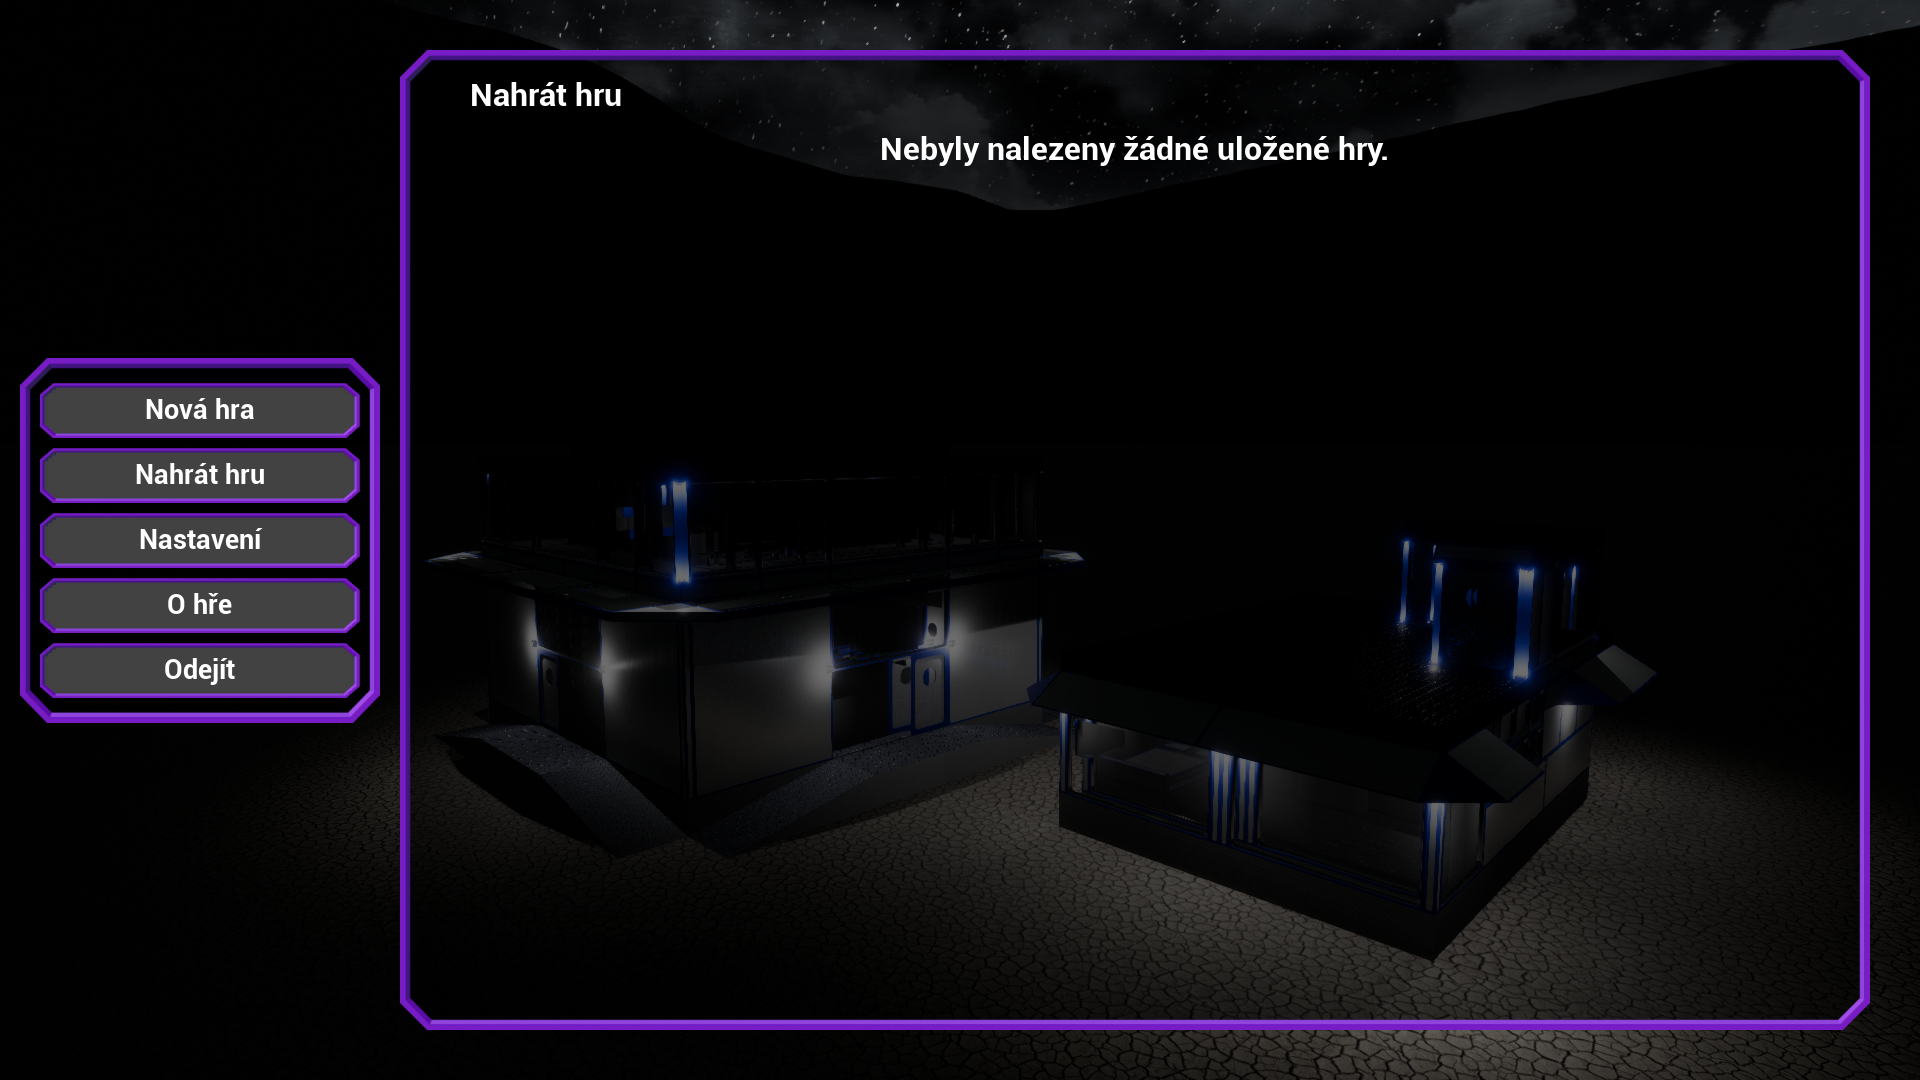
\includegraphics[ width=140mm]{../img/user/mainMenu/mmLoad}

\caption{Obrazovka hlavního menu -- Nahrát hru}
\label{fig:user_mainMenu_mmLoad}

\end{figure}
\FloatBarrier

Pod položkou \textbf{Nastavení} může uživatel měnit herní, zvuková a~grafická nastavení hry. Nastavení se aplikují a~ukládají okamžitě, výjimkou je pouze položka \textit{Animace generátoru energie}, která se projeví až po změně levelu. V~případě konfigurace z~hlavní nabídky se nastavení projeví okamžitě, v~případě konfigurace během rozehrané hry je potřeba vyvolat opětovné načtení uložené hry, nebo znovu spustit novou hru.

\begin{figure}[!ht]\centering
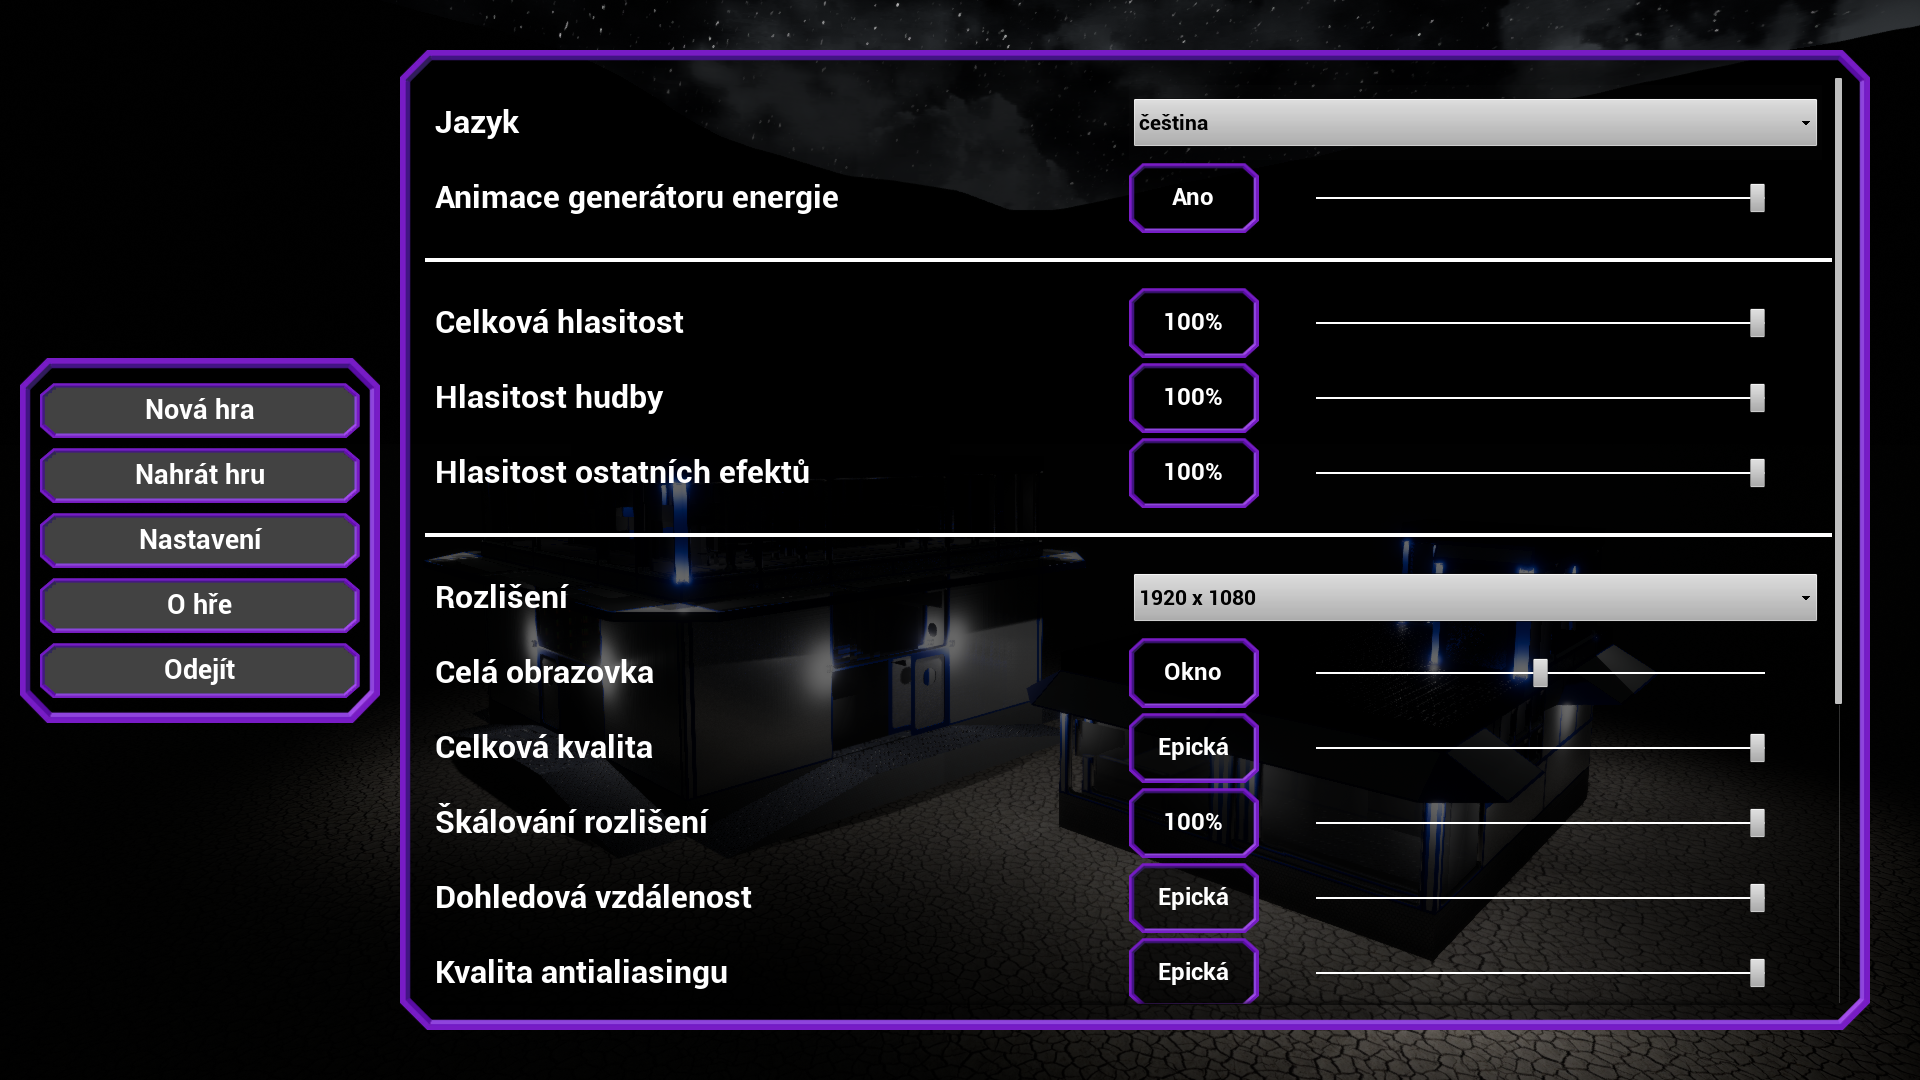
\includegraphics[ width=140mm]{../img/user/mainMenu/mmSettings}

\caption{Obrazovka hlavního menu -- Nastavení}
\label{fig:user_mainMenu_mmSettings}

\end{figure}

\FloatBarrier
%%!TEX root = ../../prace.tex

\section{Herní menu - ukládání, nahrávání}

V průběhu rozehrané hry je možné použít \textbf{Rychlé uložení / načtení}, nebo si hru uložit z~herní nabídky.

Pro uložení hry je možné vytvořit nový save nebo přepsat stávající, pokud nějaký existuje. Uložené hry je též možné mazat.

\begin{figure}[!ht]\centering
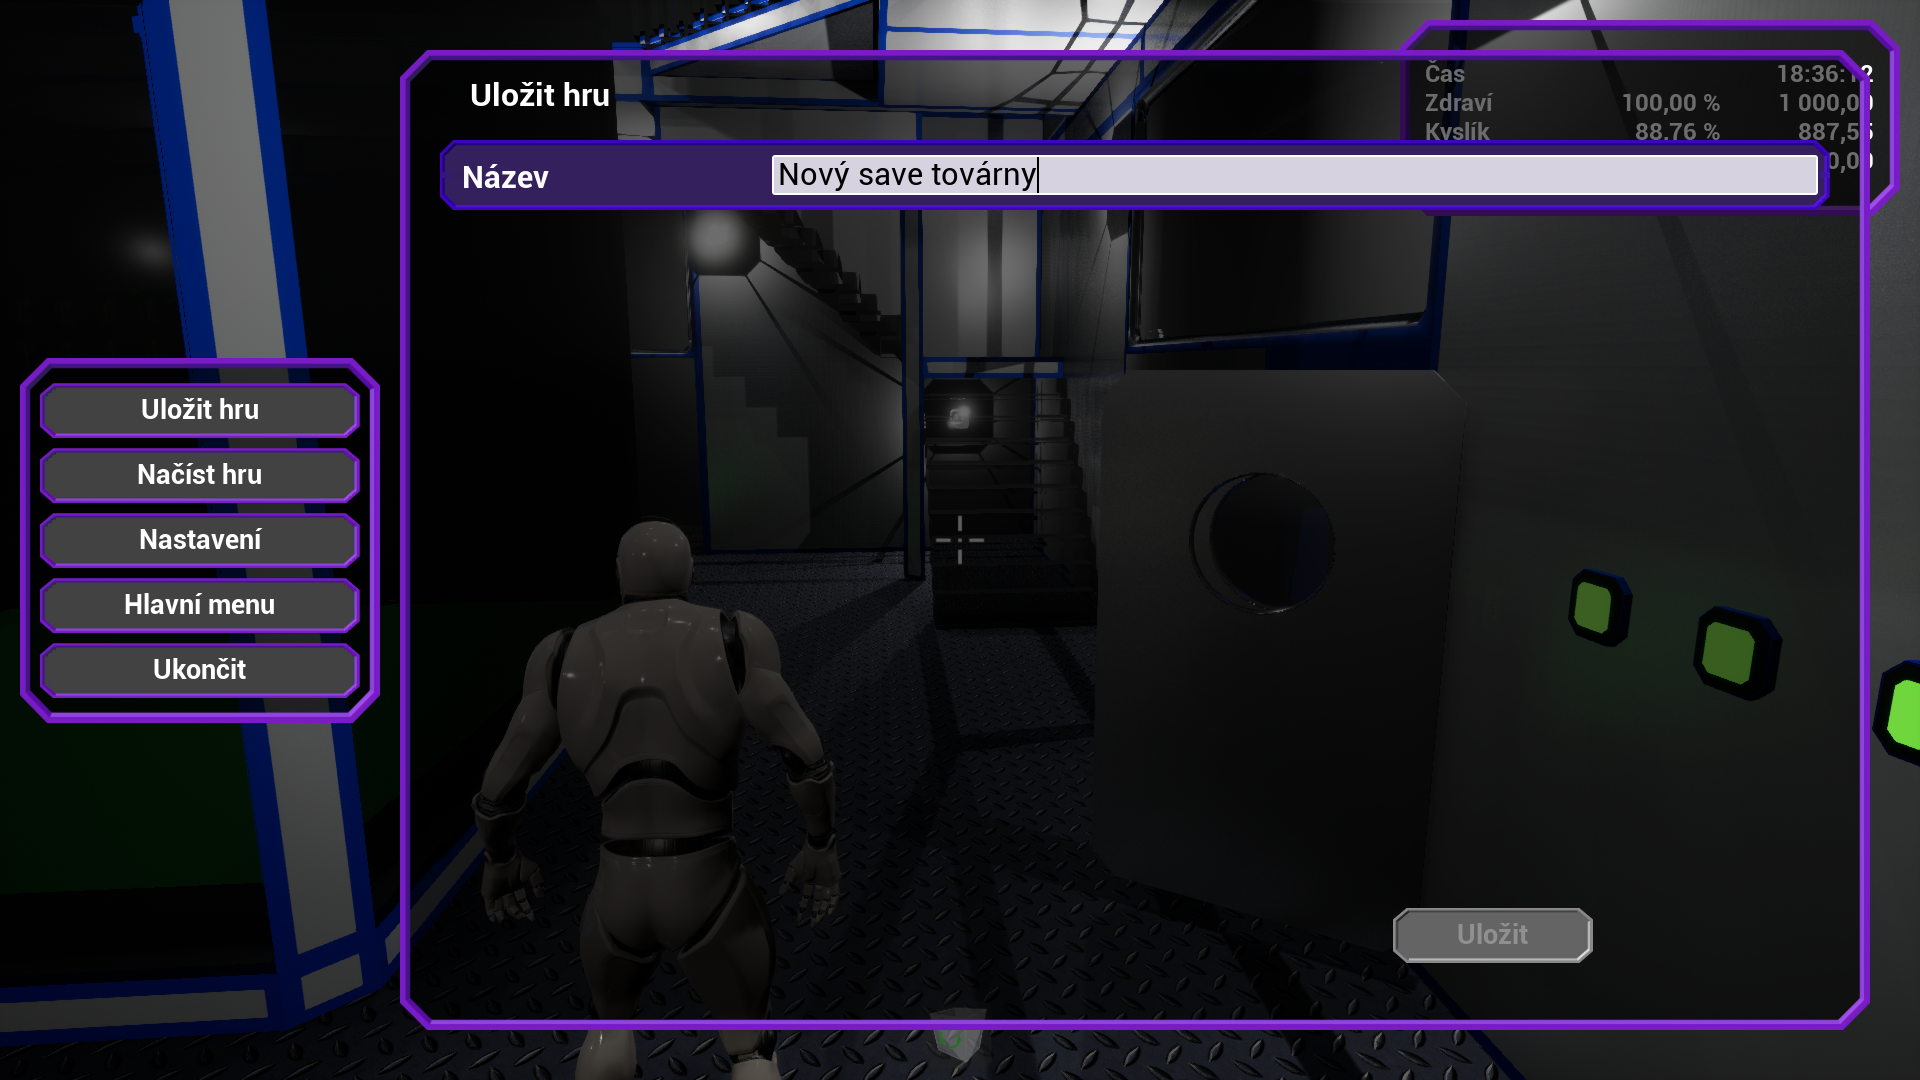
\includegraphics[ width=140mm]{../img/user/save/0newSave}

\caption{Ukládání - Nový save}
\label{fig:user_save_0newSave}

\end{figure}
\FloatBarrier

Pokud bylo uložení úspěšné, hráči se zobrazí následující hláška:

\begin{figure}[!ht]\centering
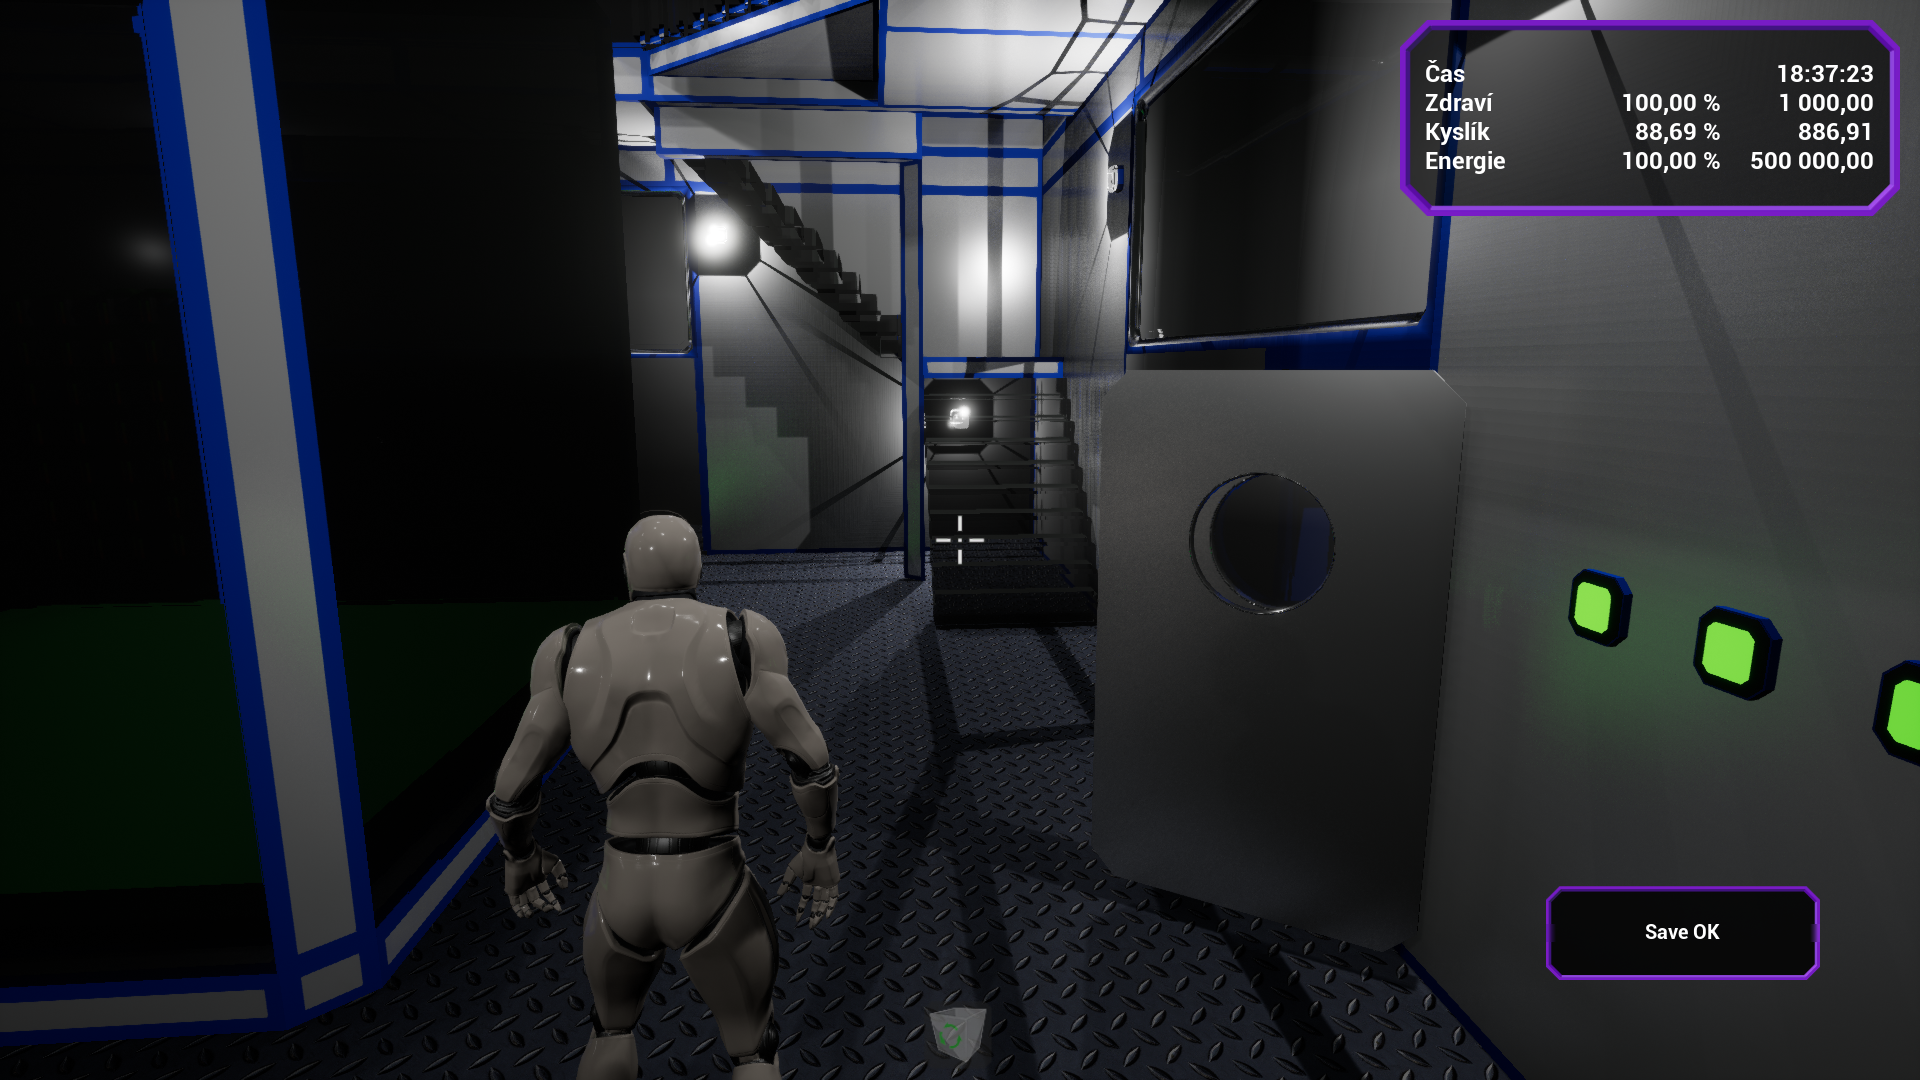
\includegraphics[ width=140mm]{../img/user/save/1afterSave}

\caption{Ukládání - po uložení}
\label{fig:user_save_1afterSave}

\end{figure}
\FloatBarrier

Nahrávat je možné ze všech uložených pozic, včetně rychlého uložení. Opět je zde možné vybraný save smazat.

\begin{figure}[!ht]\centering
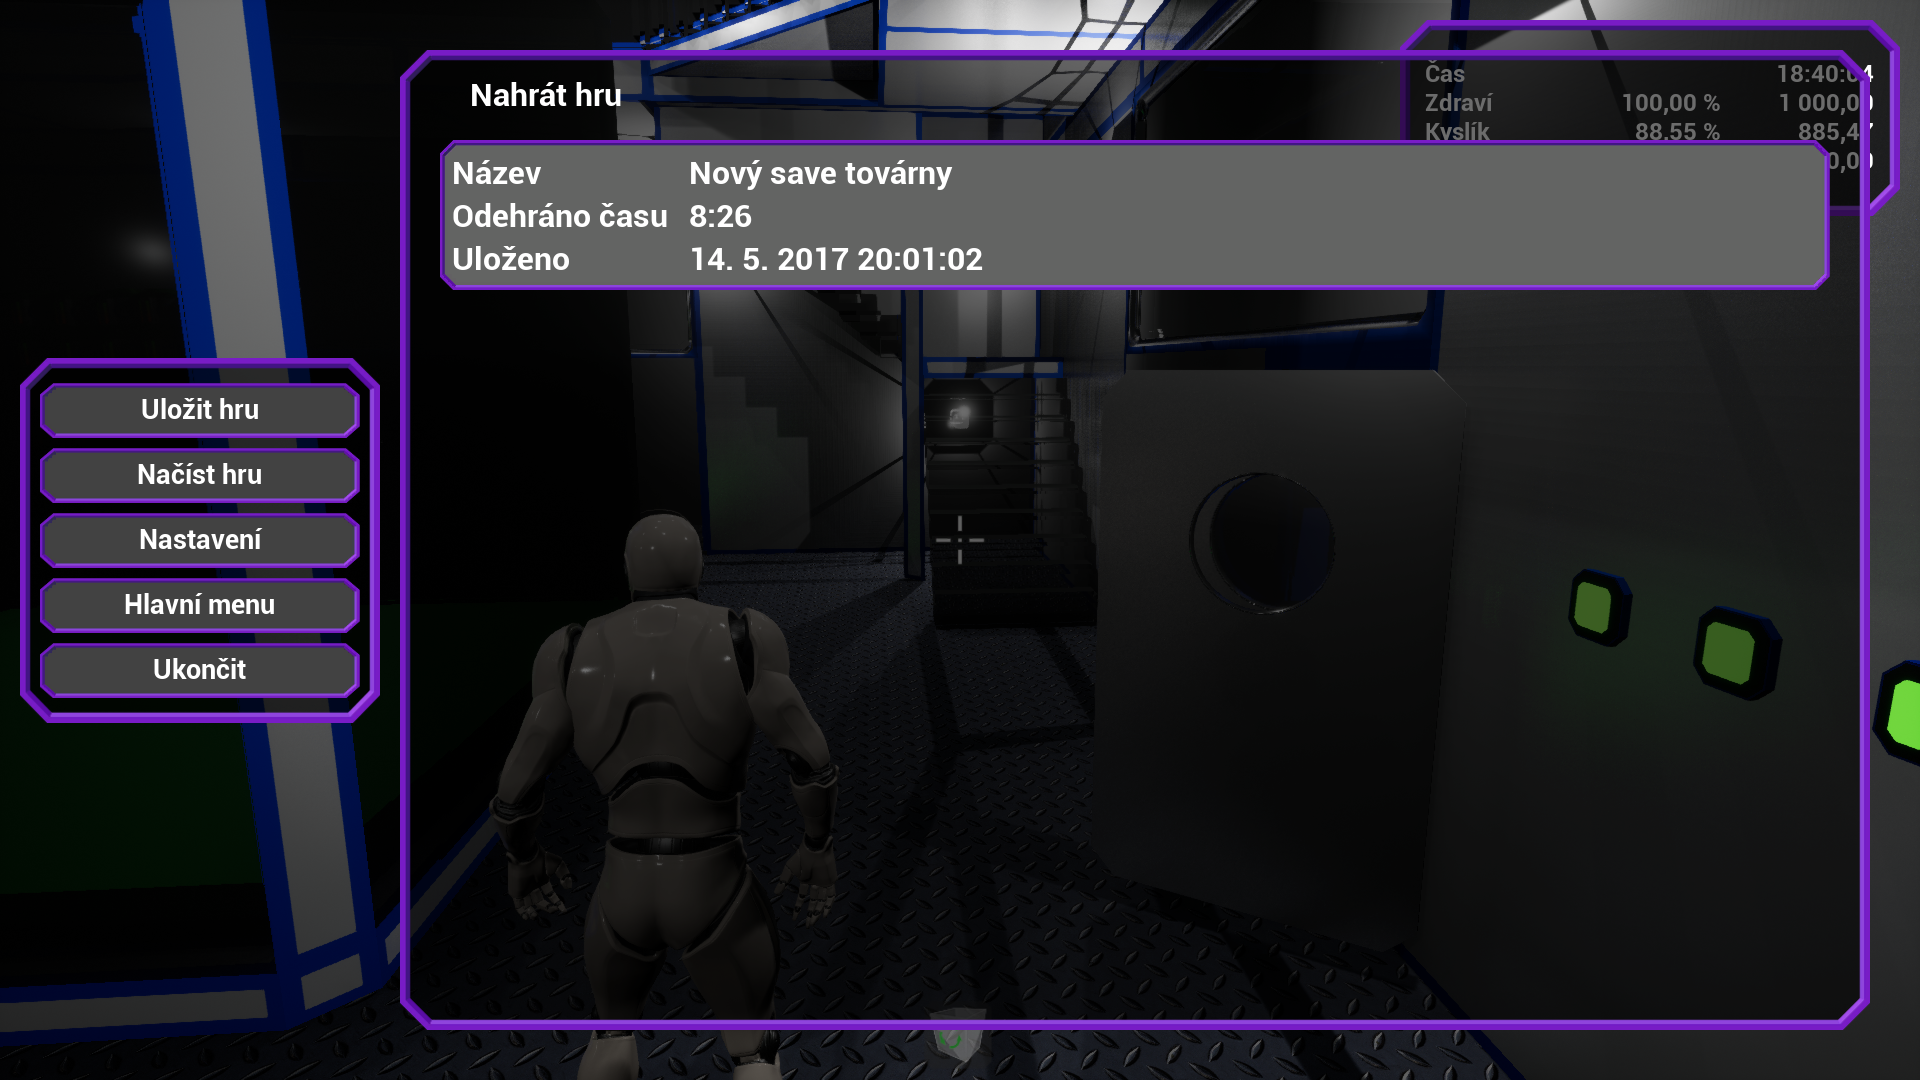
\includegraphics[ width=140mm]{../img/user/save/2load}

\caption{Ukládání - nahrát hru}
\label{fig:user_save_2load}

\end{figure}
\FloatBarrier

Pokud má hráč rozehranou hru, je pro jistotu vyžadováno potvrzení.

\begin{figure}[!ht]\centering
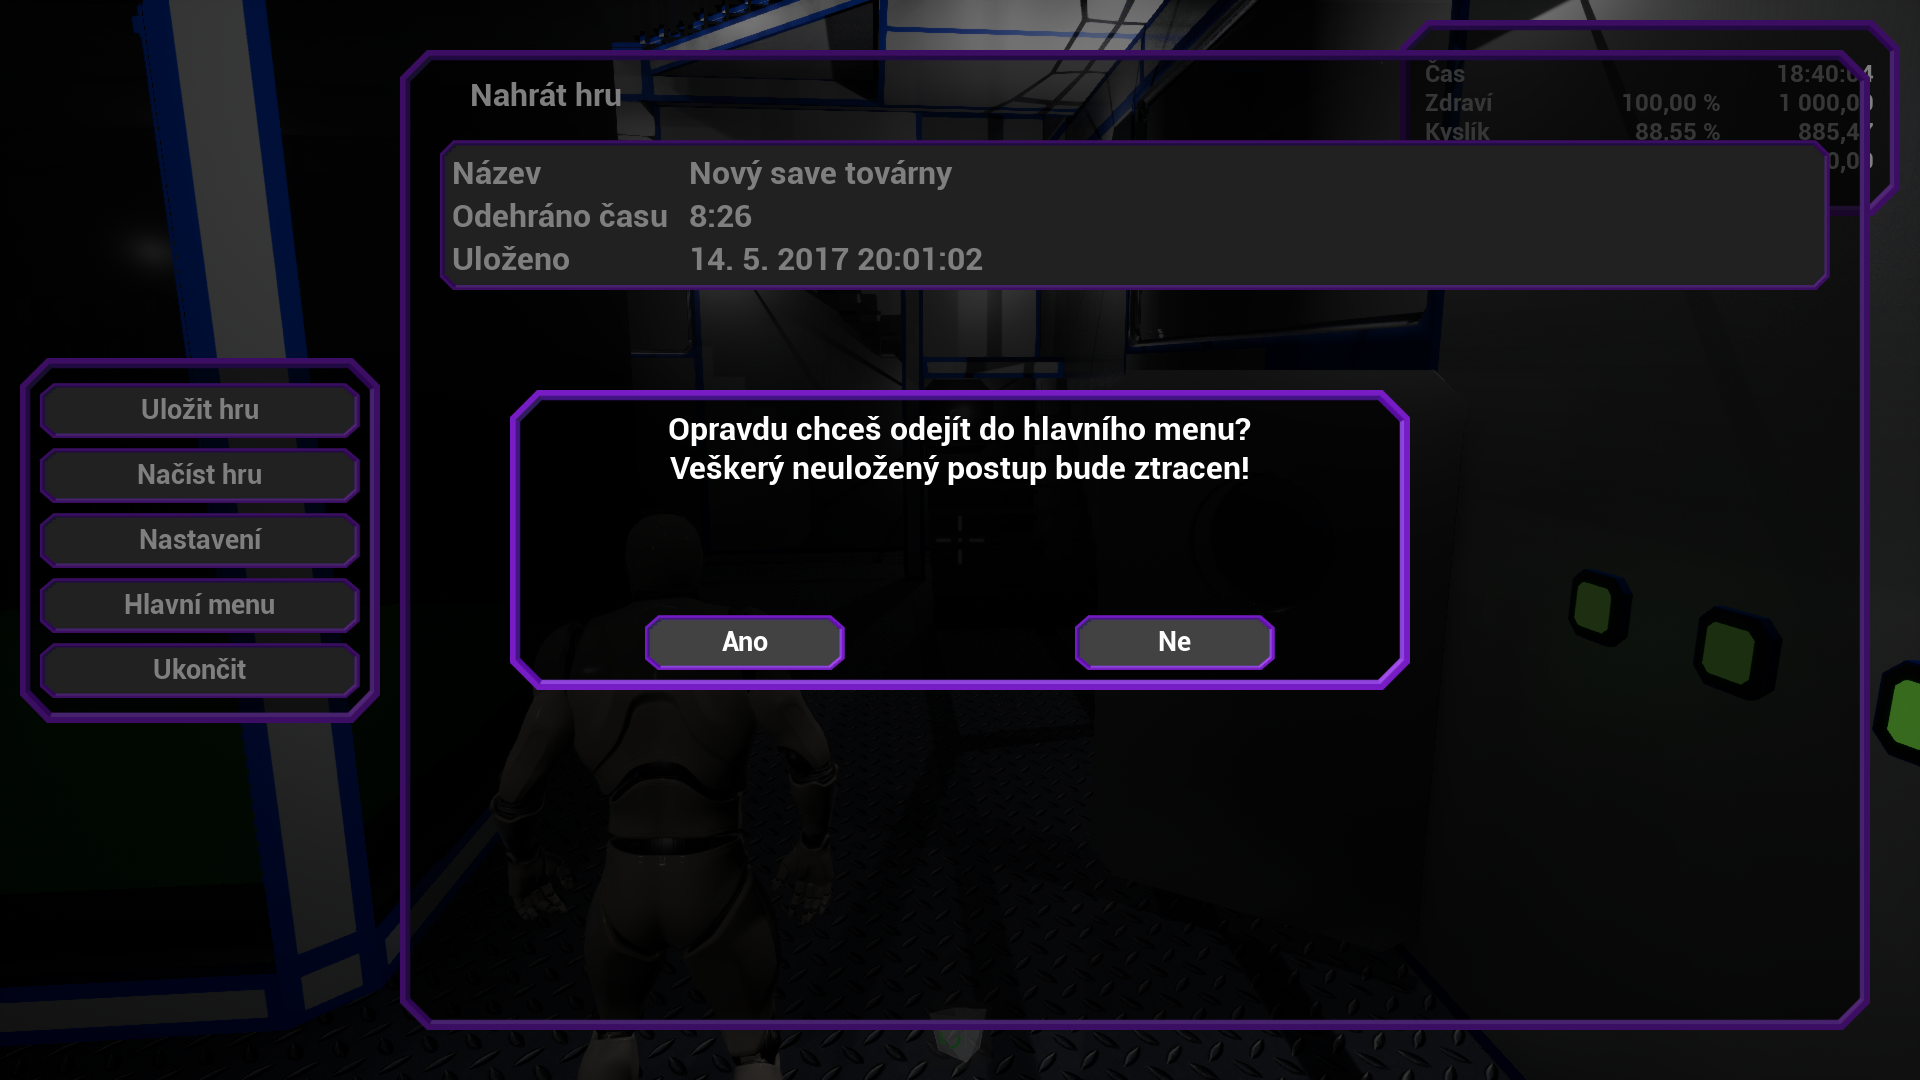
\includegraphics[ width=140mm]{../img/user/save/3loadClicked}

\caption{Ukládání - potvrzení nahrání hry}
\label{fig:user_save_3loadClicked}

\end{figure}

\FloatBarrier
%%!TEX root = ../../prace.tex

\section{Inventář}

Inventář se vyvolá klávesou \textbf{E}. Zobrazí se následující obrazovka:

\begin{figure}[!ht]\centering
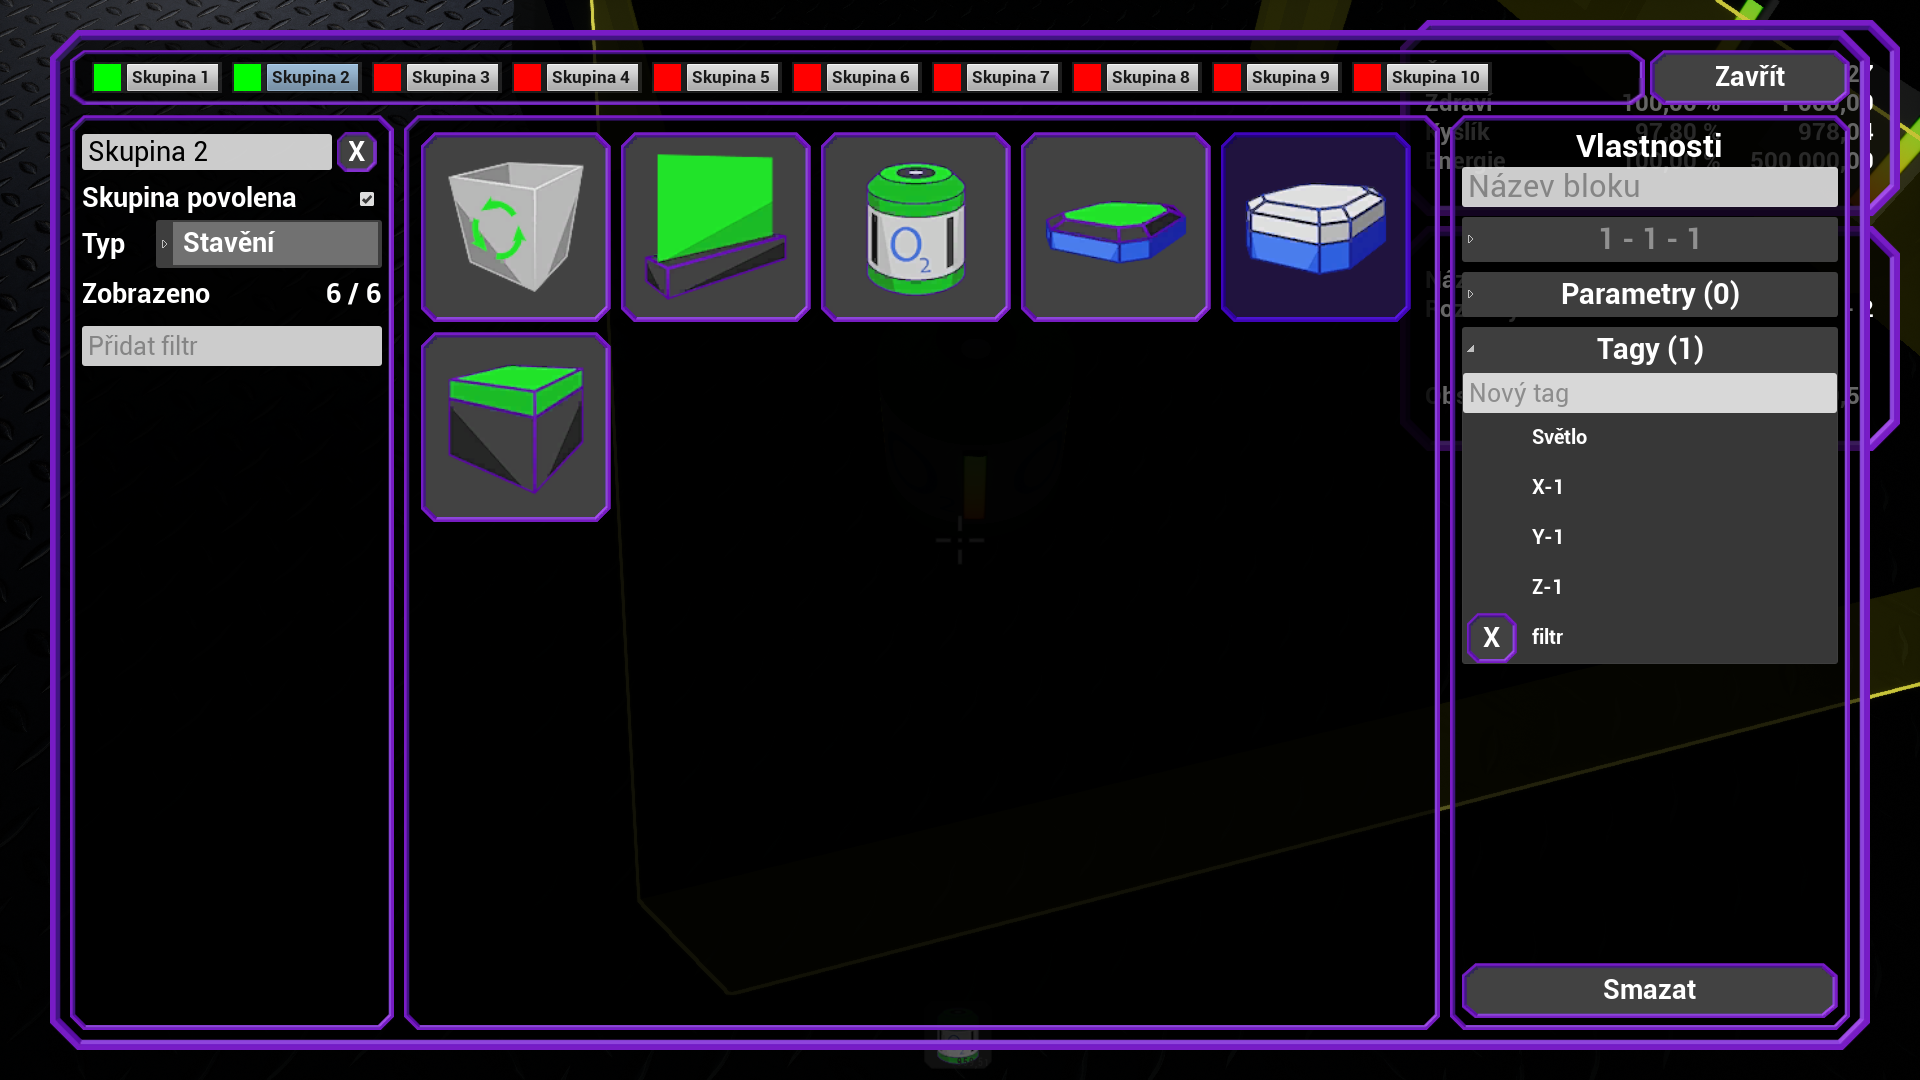
\includegraphics[ width=140mm]{../img/user/inventory/0AddTag}

\caption{Inventář - přehled}
\label{fig:user_inventory_0AddTag}

\end{figure}

\FloatBarrier

V horní části je výběr skupin. Je možné vybírat z 10 skupin, které si lze pojmenovat dle libosti. Dále je možné je (de)aktivovat buď kliknutím na zelený / červený čtverec, nebo skrze příslušný checkbox v editaci skupiny.
Je možné používat standardní změnu skupiny klávesami \textbf{ú} a \textbf{)}, editační okno se pak příslušným způsobem změní. 

V \textit{levé} části je \textbf{editor skupiny}, jehož funkce budou popsány v textu dále. \textit{Uprostřed} je možné vidět postavitelné či umístitelné položky, které jsou dofiltrovány dle právě nastaveného filtru. Výběrem položky lze editovat její vlastnosti v \textit{pravé} části okna

\FloatBarrier

Každá skupina umožňuje definovat své filtry. Matematicky bychom mohli popsat filtrování jako vyhodnocení formule v \textit{CNF}. Pokud do pole \textit{Přidat filtr} napíšeme tagy oddělené mezerou, do skupiny se přidá \textbf{nová} skupina s výchozím pojmenováním.

\begin{figure}[!ht]\centering
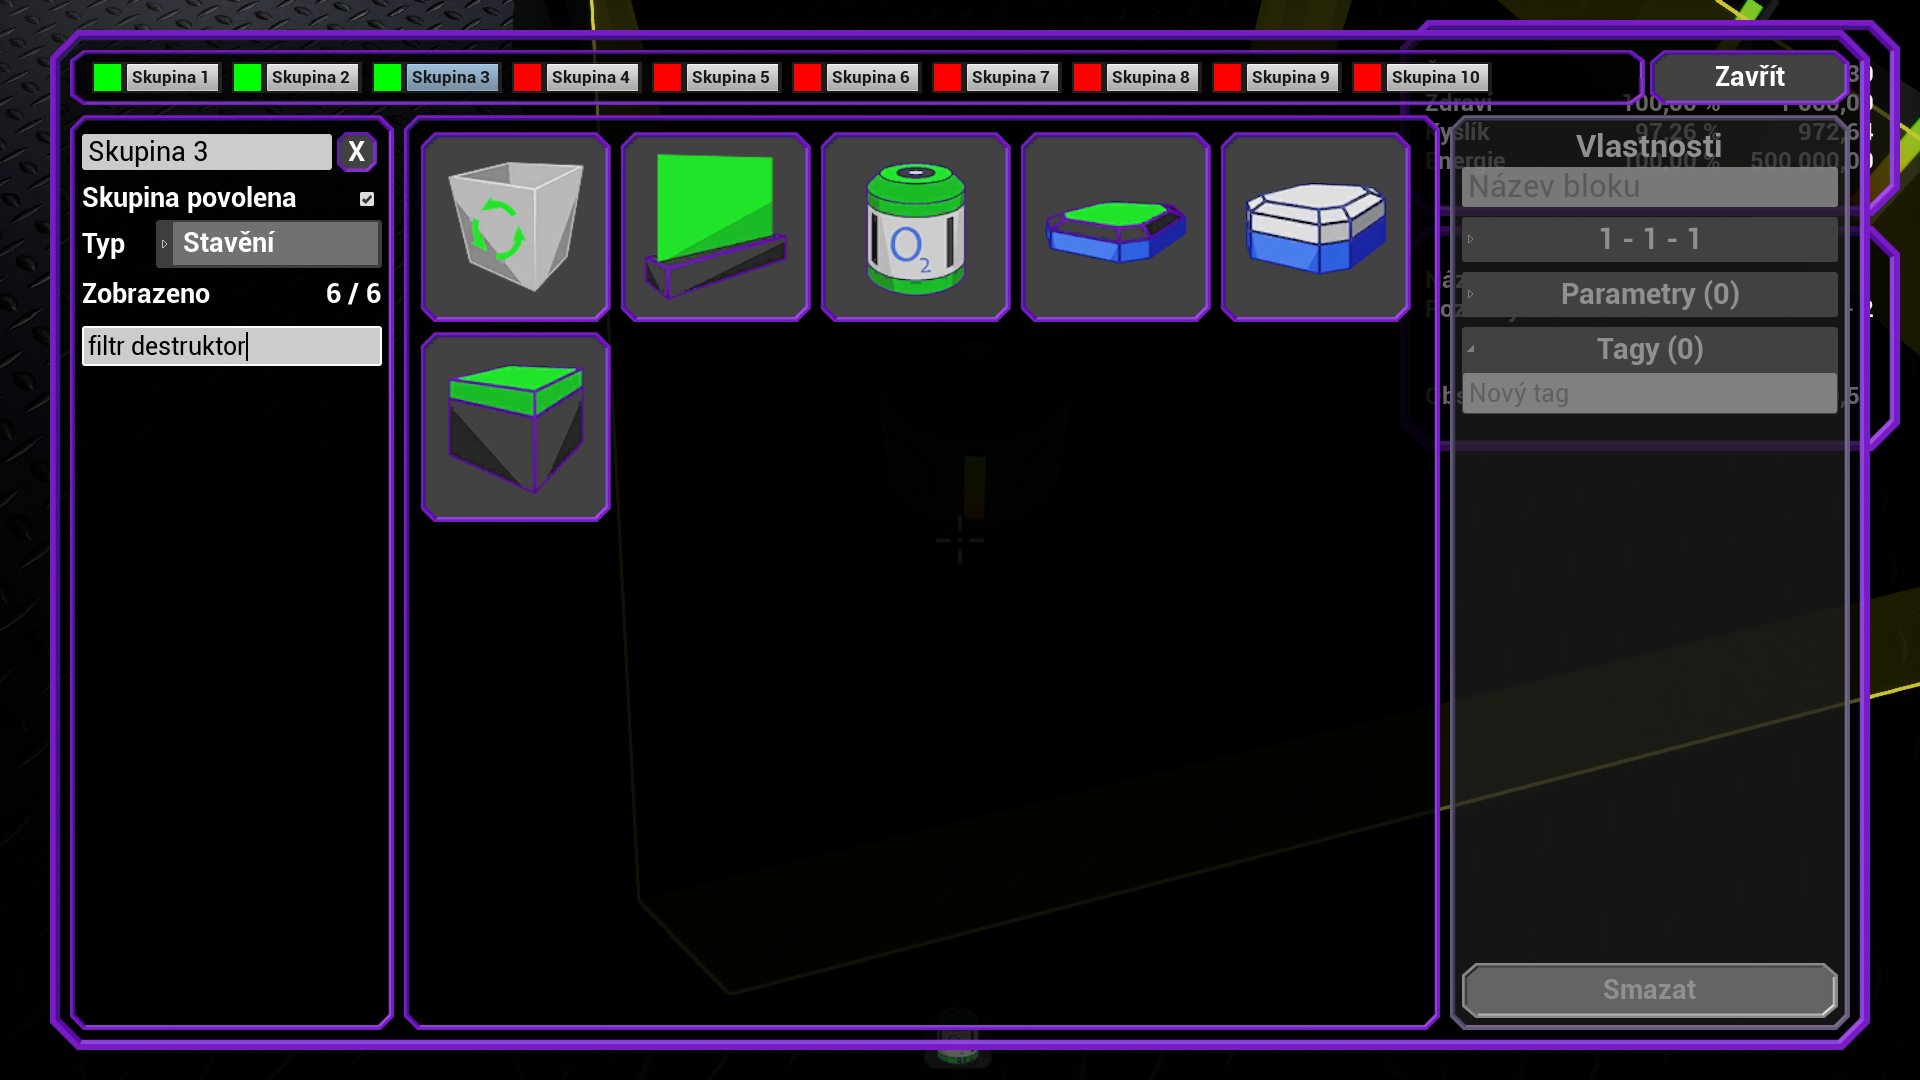
\includegraphics[ width=140mm]{../img/user/inventory/1setFilter}

\caption{Inventář - přidání skupiny}
\label{fig:user_inventory_1setFilter}

\end{figure}

\FloatBarrier

Po přidání se seznam dostupných prvků dofiltruje podle nastavených tagů - ve výsledku bude každá položka splňovat alespoň jeden tag z každé skupiny. Shoda nemusí být přesná, tag objektu musí obsahovat podřetězec definovaný filtrem.
\begin{figure}[!ht]\centering
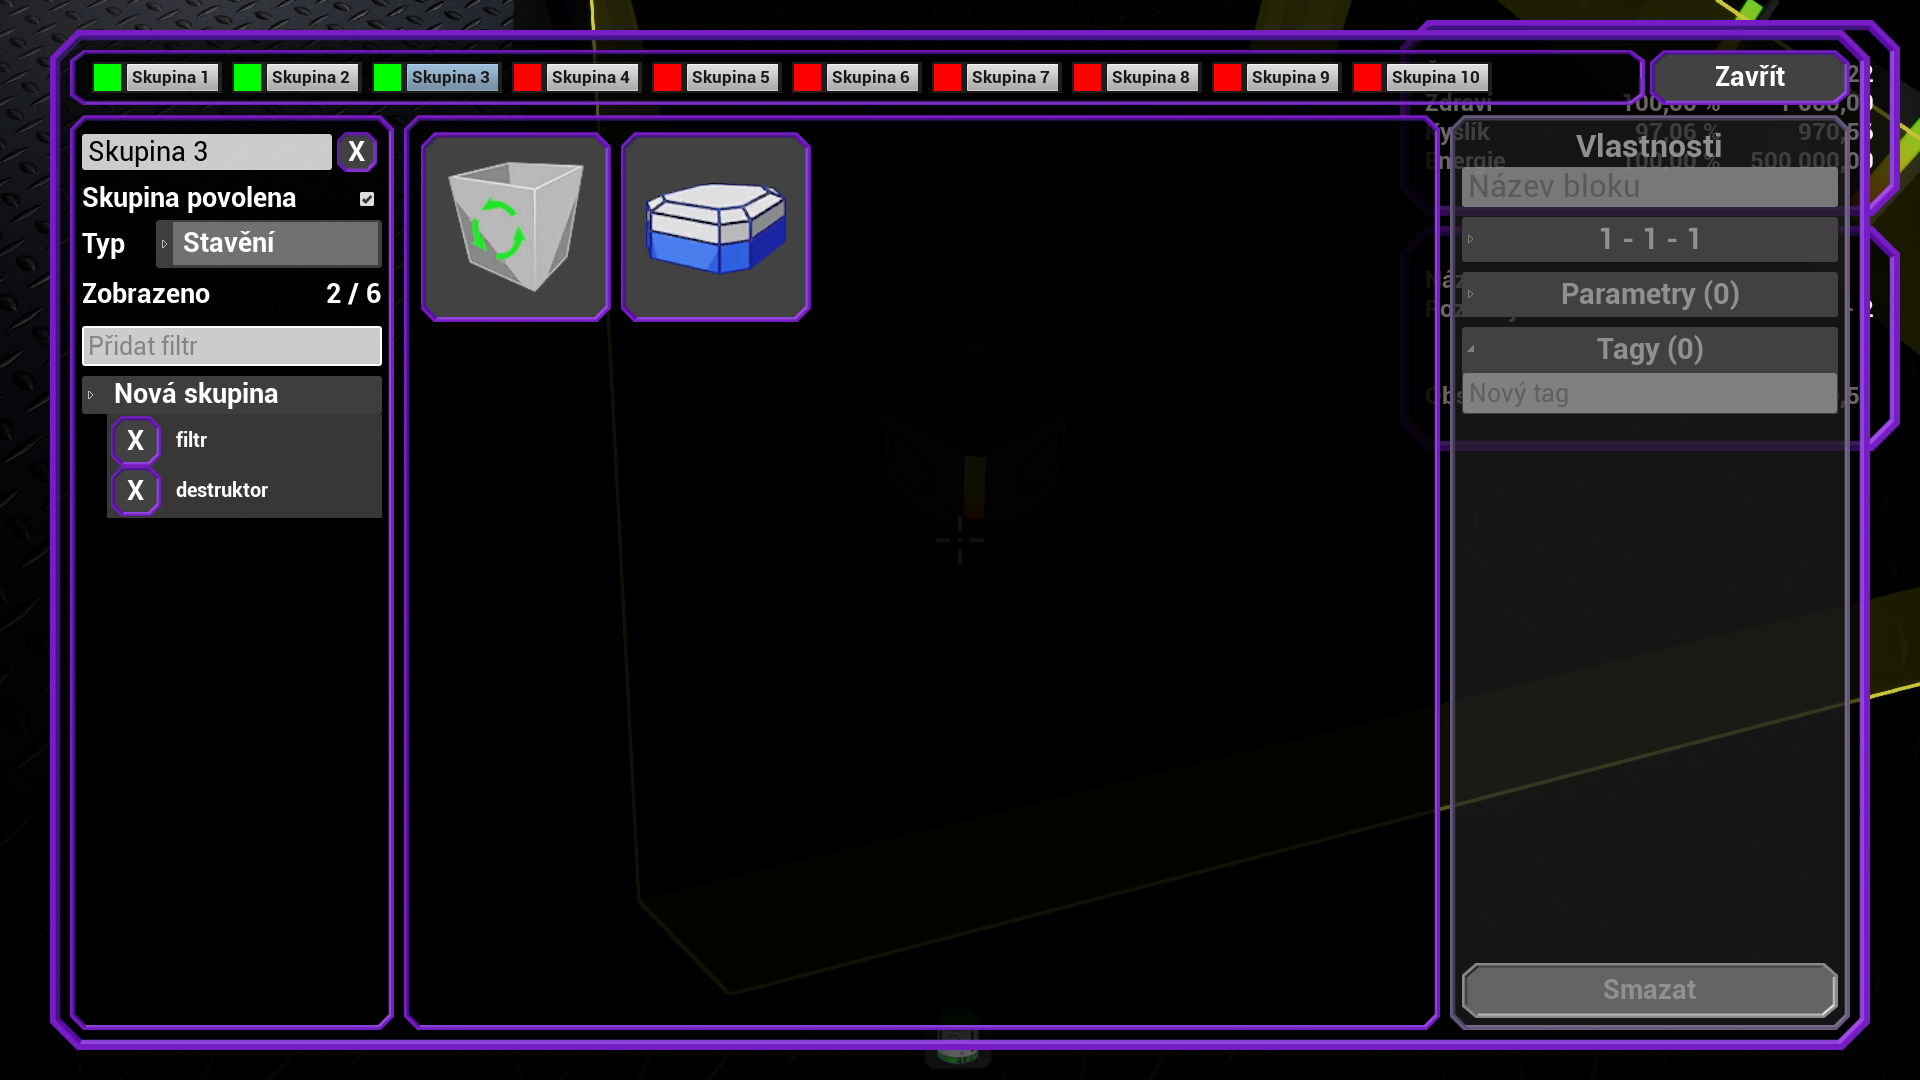
\includegraphics[ width=140mm]{../img/user/inventory/2filterResult}

\caption{Inventář - výsledek s filtrovanými položkami}
\label{fig:user_inventory_2filterResult}

\end{figure}

\FloatBarrier

Na následujícím obrázku je možné vidět filtry s rozbalenými vlastnostmi. Zaměřme se nyní na část \textit{Nesbalovat}. Po zaškrtnutí této volby je zobrazena pouze hlavička skupiny.

\begin{figure}[!ht]\centering
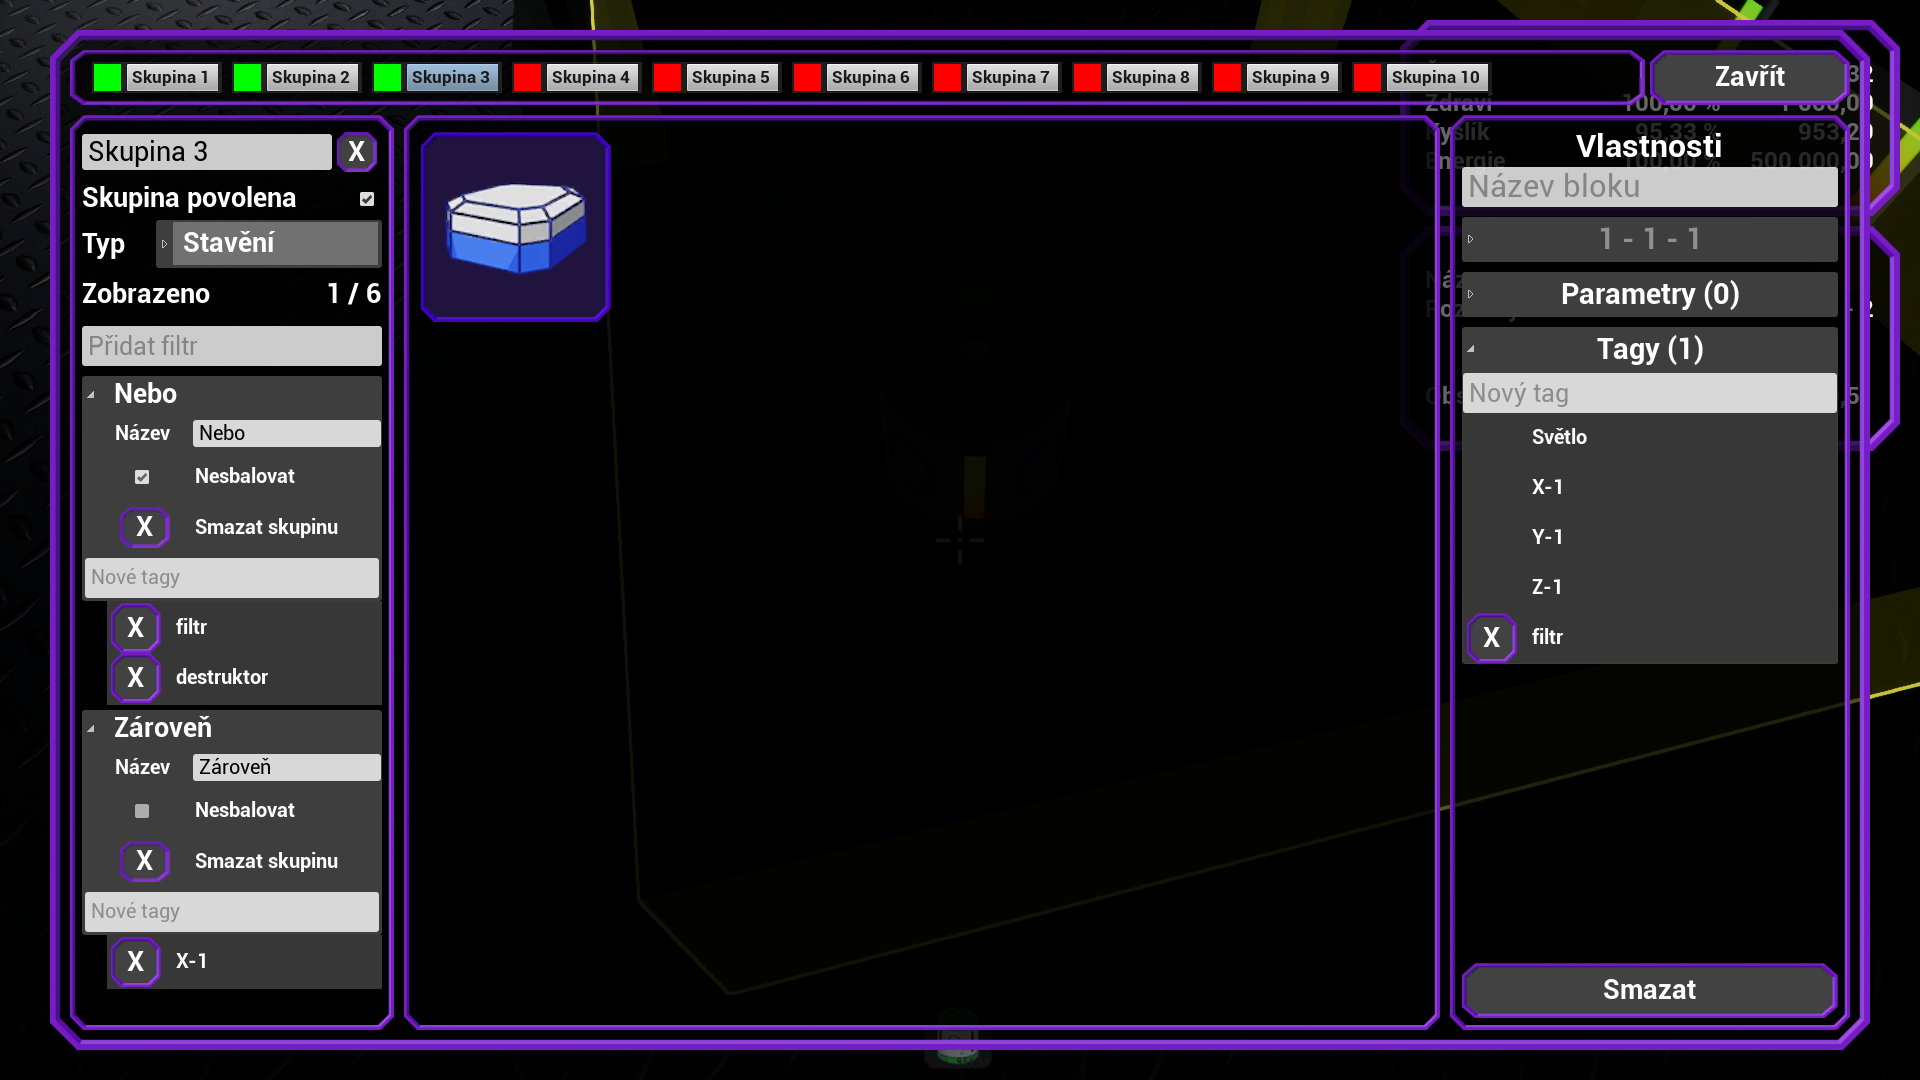
\includegraphics[ width=140mm]{../img/user/inventory/3additionalFilter}

\caption{Inventář - Nová hra}
\label{fig:user_inventory_3additionalFilter}

\end{figure}

\FloatBarrier

Výsledný seznam se sbalenými vlastnostmi filtru:

\begin{figure}[!ht]\centering
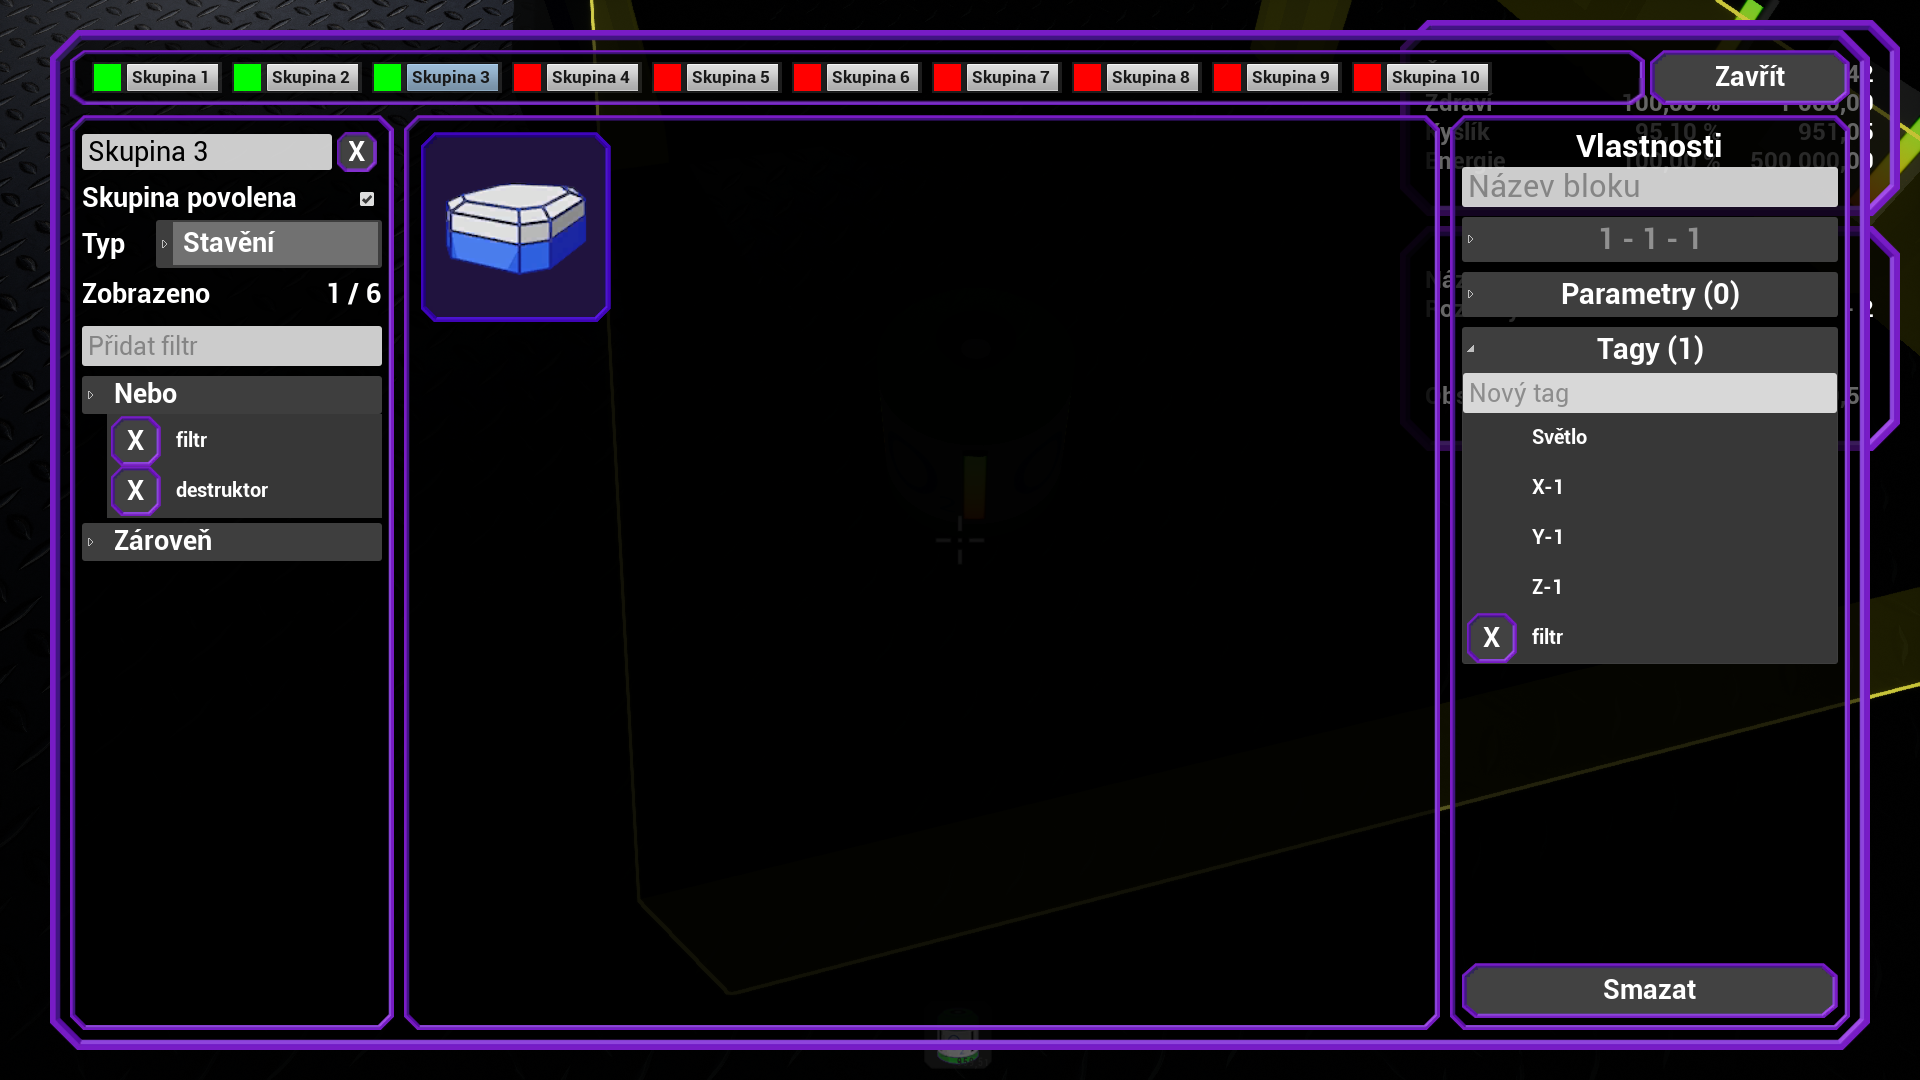
\includegraphics[ width=140mm]{../img/user/inventory/4addFilterCollapsed}

\caption{Inventář - Nahrát hru}
\label{fig:user_inventory_4addFilterCollapsed}

\end{figure}

\FloatBarrier

Označené položky je také možné smazat z inventáře. Umístitelné položky tak mohou být reálně zničeny. 

\begin{figure}[!ht]\centering
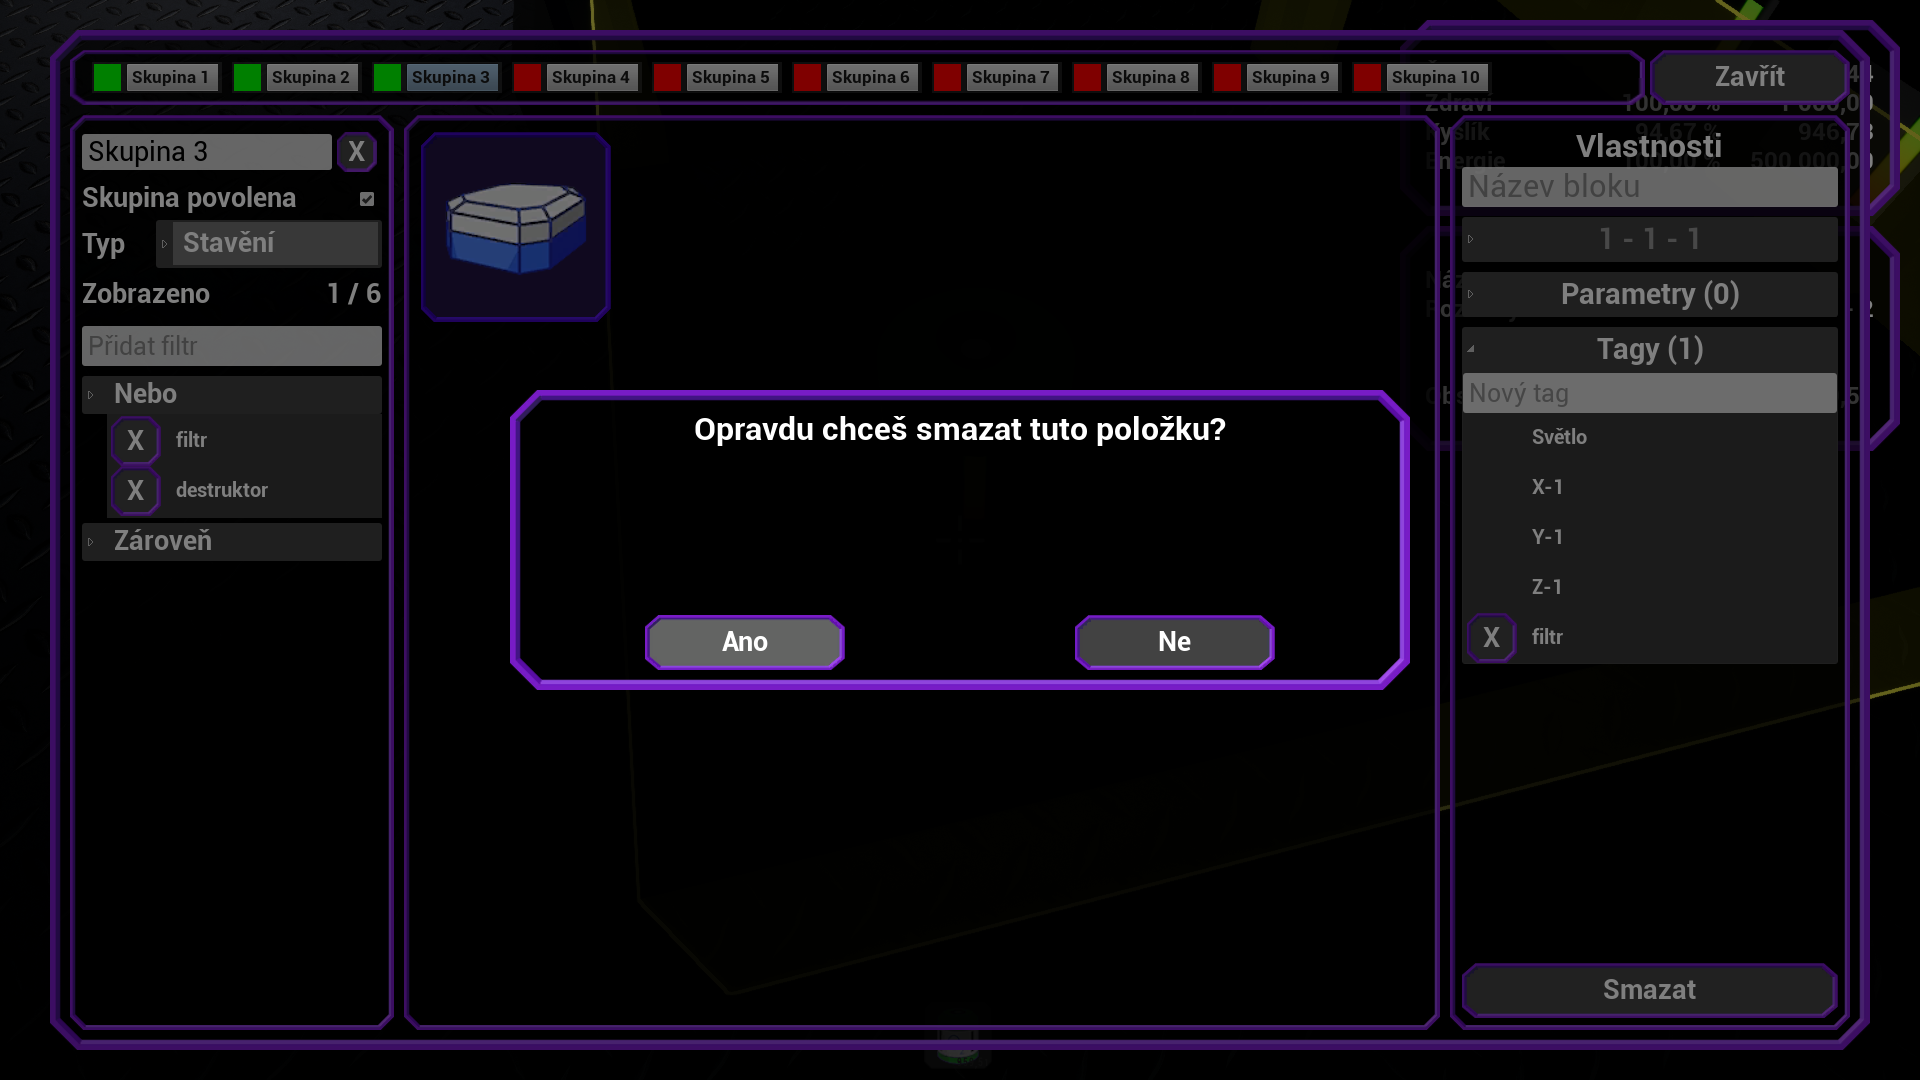
\includegraphics[ width=140mm]{../img/user/inventory/5deleteItem}

\caption{Inventář - Nastavení}
\label{fig:user_inventory_5deleteItem}

\end{figure}

\FloatBarrier
V případě, že je zvolena položka s dodatečnými parametry, je možné jejich hodnoty vidět v editoru vlastností bloku

\begin{figure}[!ht]\centering
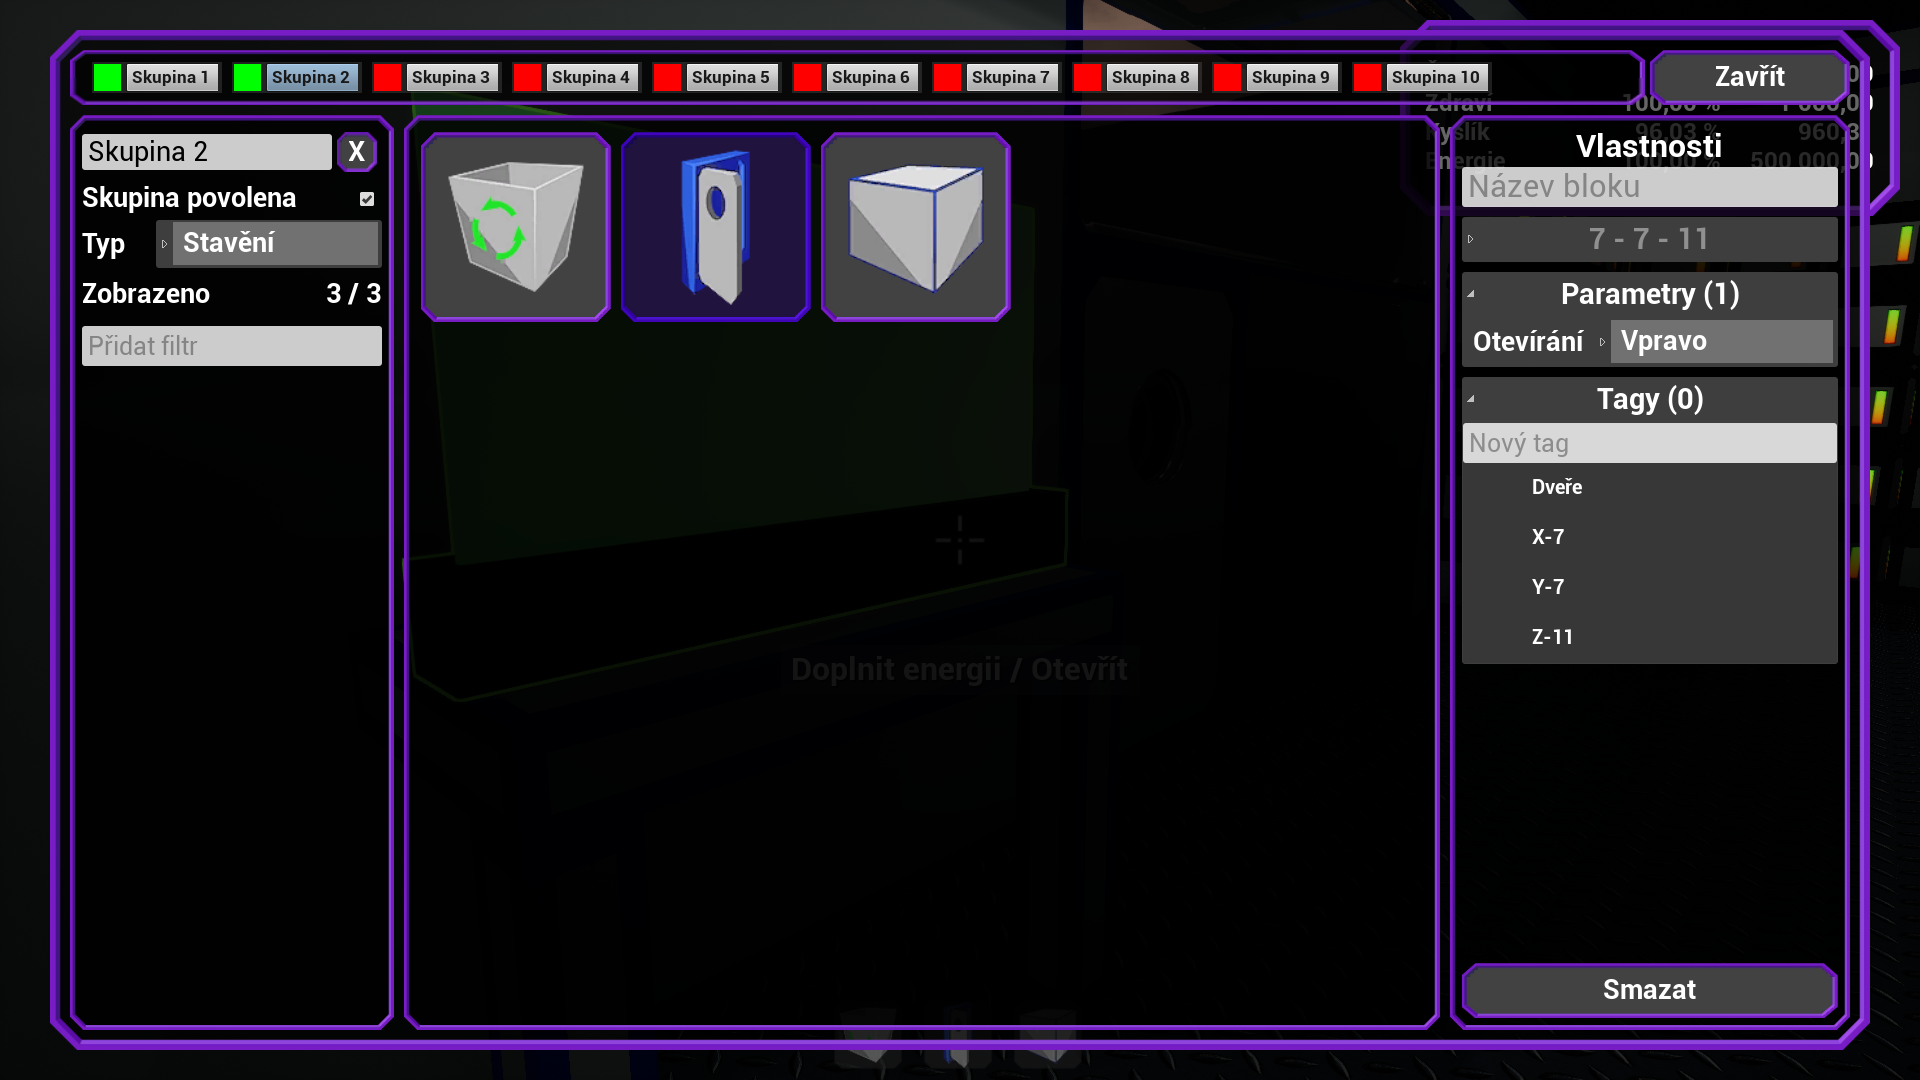
\includegraphics[ width=140mm]{../img/user/inventory/6itemWithParams}

\caption{Inventář - Nastavení}
\label{fig:user_inventory_6itemWithParams}

\end{figure}


\FloatBarrier
%%!TEX root = ../prace.tex

\section{Terminál}

Pro informaci o aktuálním stavu sítě je nutné použít \textbf{Terminál}. Levým tlačítkem je možné rychle doplnit energii hráče, pravým pak otevřít ovládací obrazovku.

\begin{figure}[!h]\centering
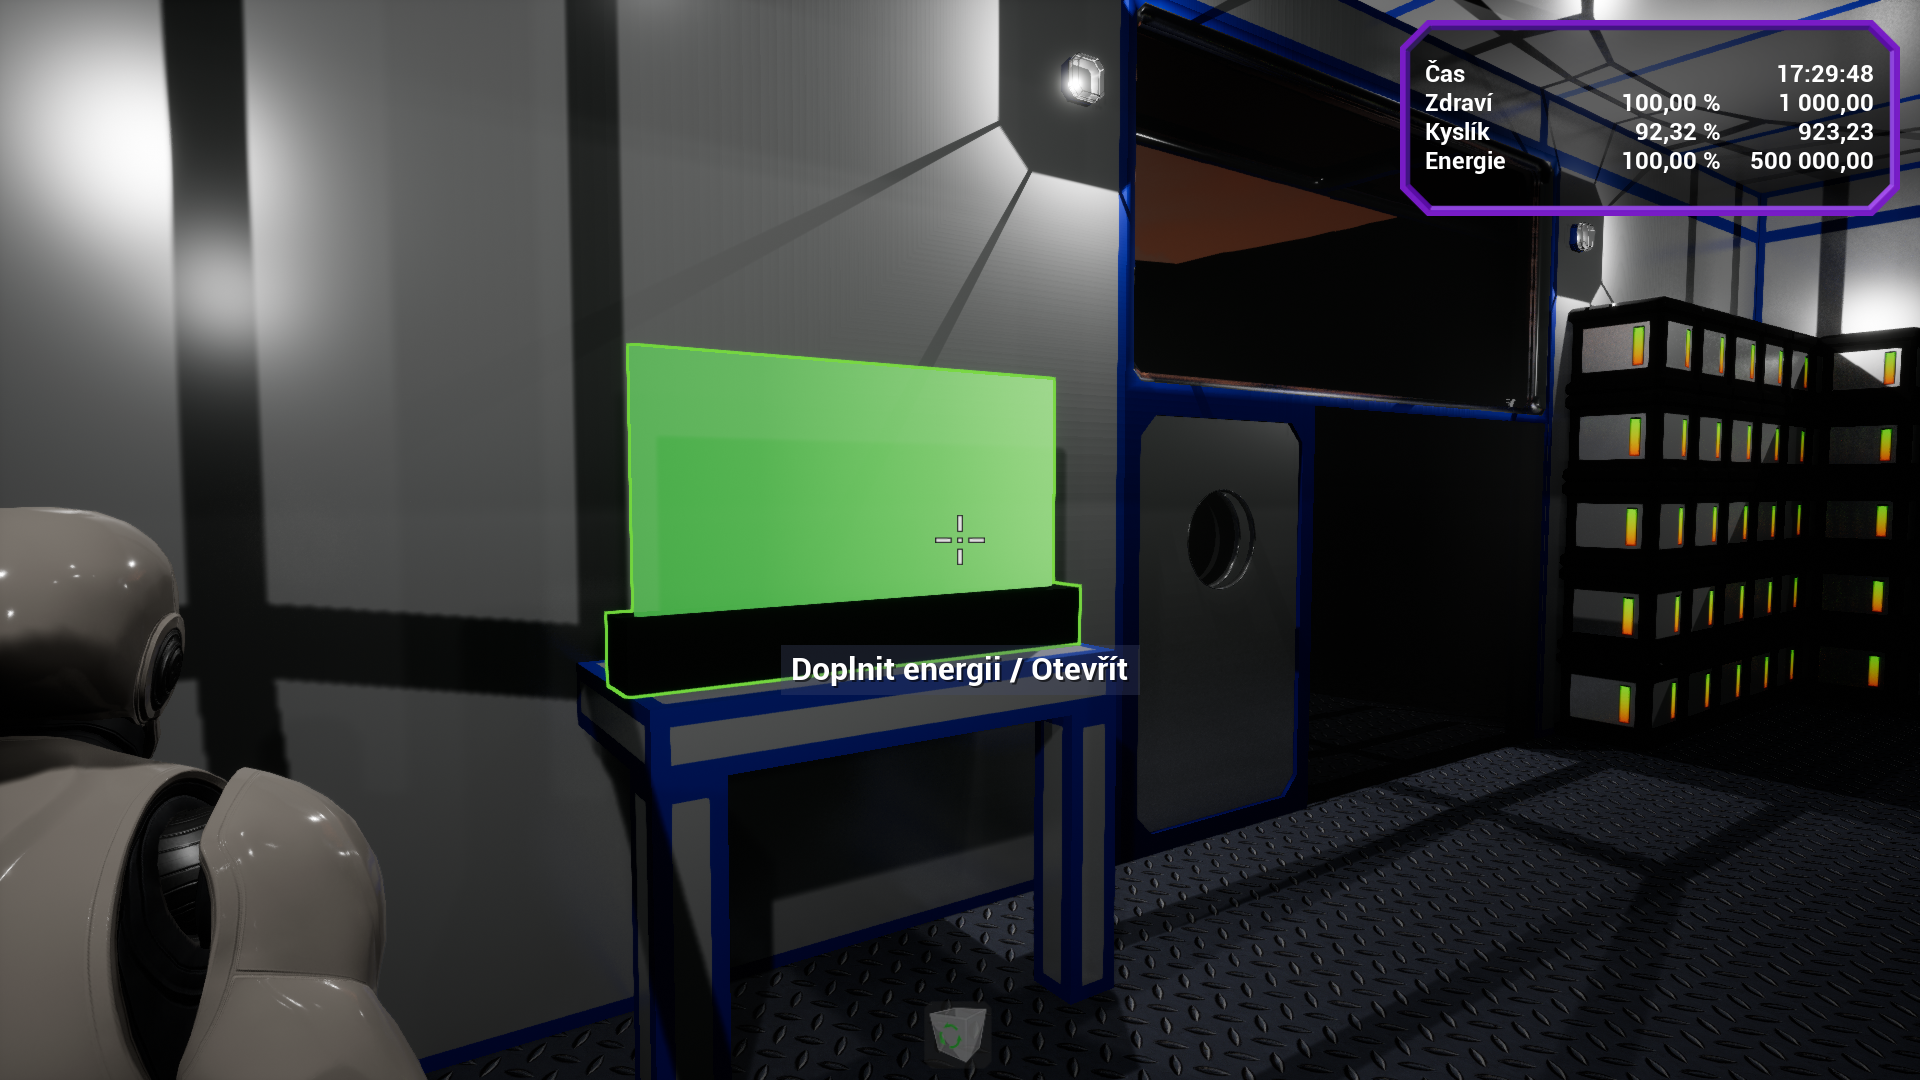
\includegraphics[ width=140mm]{../img/user/terminal/0terminalOverall}

\caption{Terminál - ve hře}
\label{fig:user_terminal_0terminalOverall}

\end{figure}

\FloatBarrier

V \textit{horní} části je vidět selektor obrazovky. Jeho rozkliknutím (více v obrázku \ref{fig:user_terminal_3terminalCtorSelector}) je možné zvolit výchozí obrazovku, nebo jeden z \textbf{Konstruktoru objektů}, které jsou v dispozici v síti.




\begin{figure}[!h]\centering
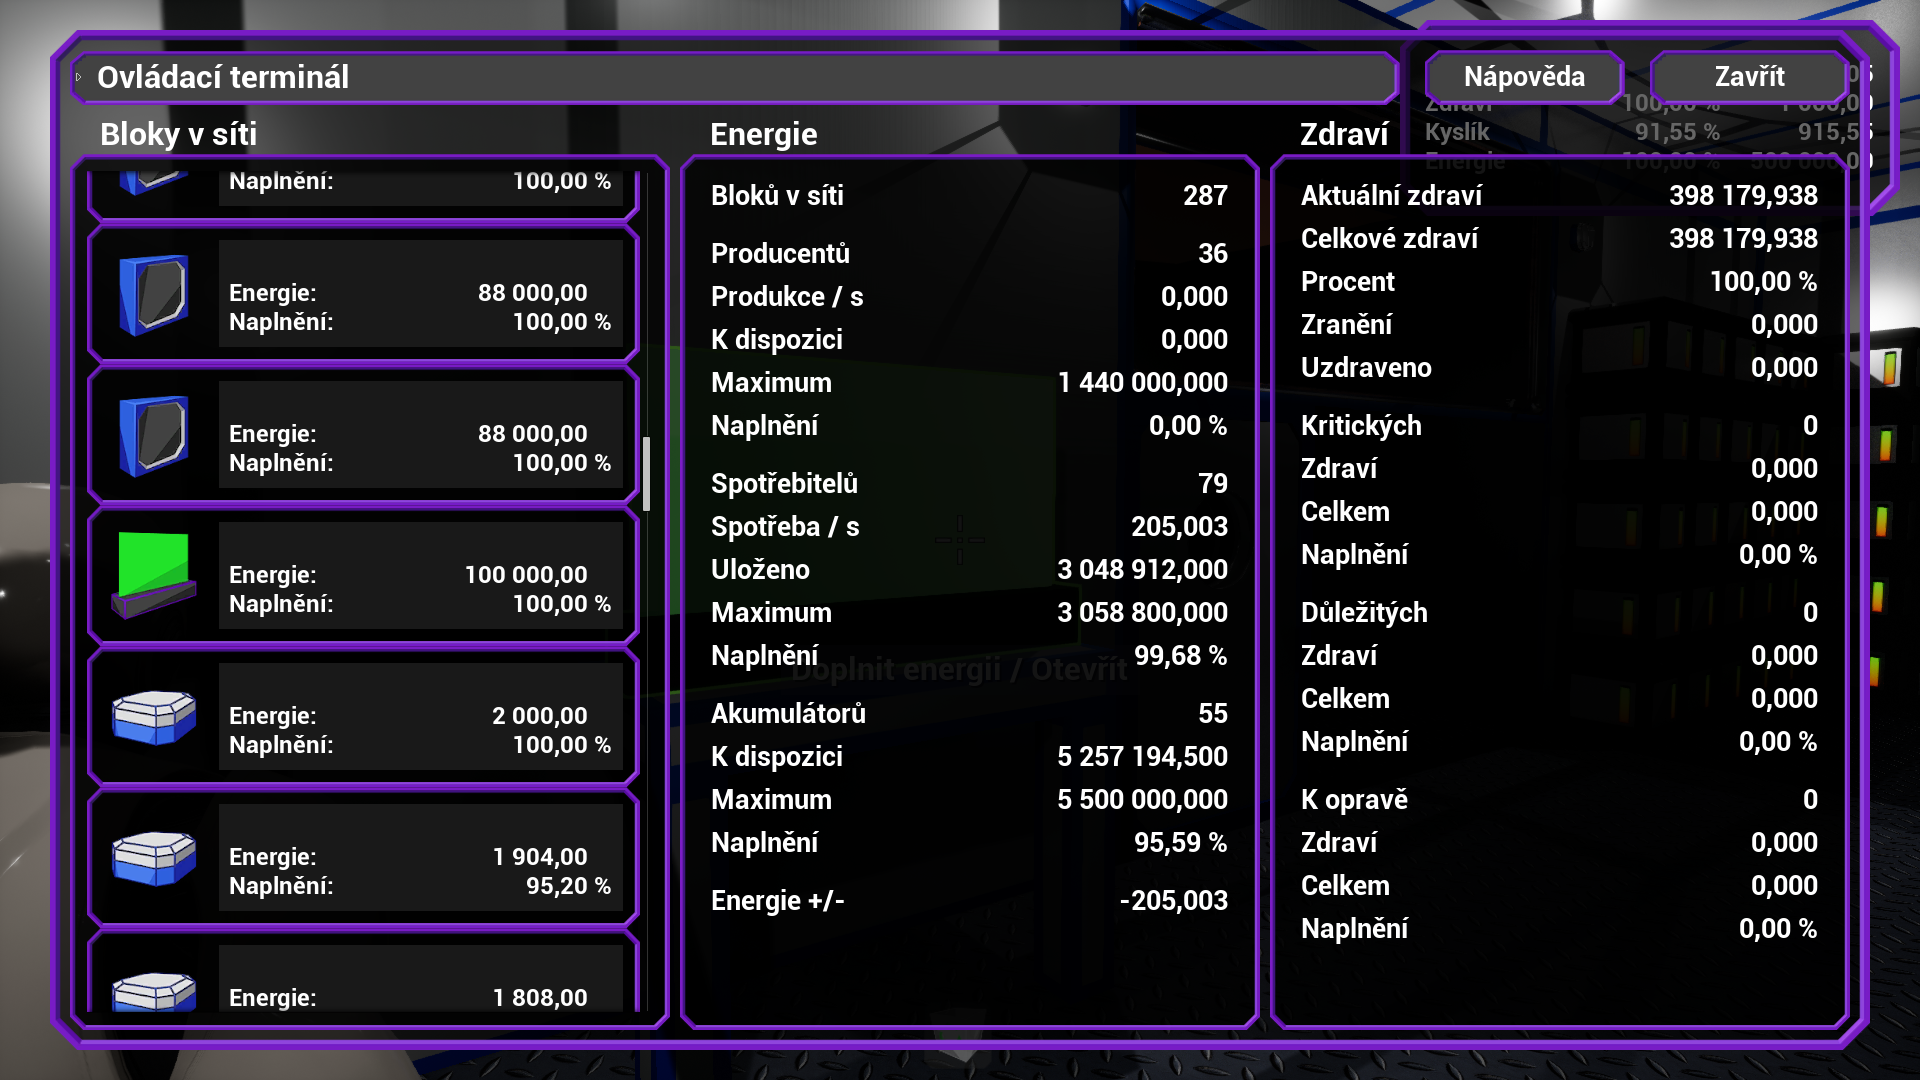
\includegraphics[ width=140mm]{../img/user/terminal/1terminalInfo}

\caption{Terminál - výchozí obrazovka}
\label{fig:user_terminal_1terminalInfo}

\end{figure}

\FloatBarrier
V \textit{levé} části je vidět seznam význačných bloků. \textit{Uprostřed} jsou vidět energetické informace o síti. \textit{Vpravo} je pak možné sledovat aktuální zdravotní stav sítě a bloků v síti.

Tlačítkem \textbf{Nápověda} je možné zobrazit informace o ovládání hry a přiřazených klávesách pro jednotlivé úkony.

\begin{figure}[!h]\centering
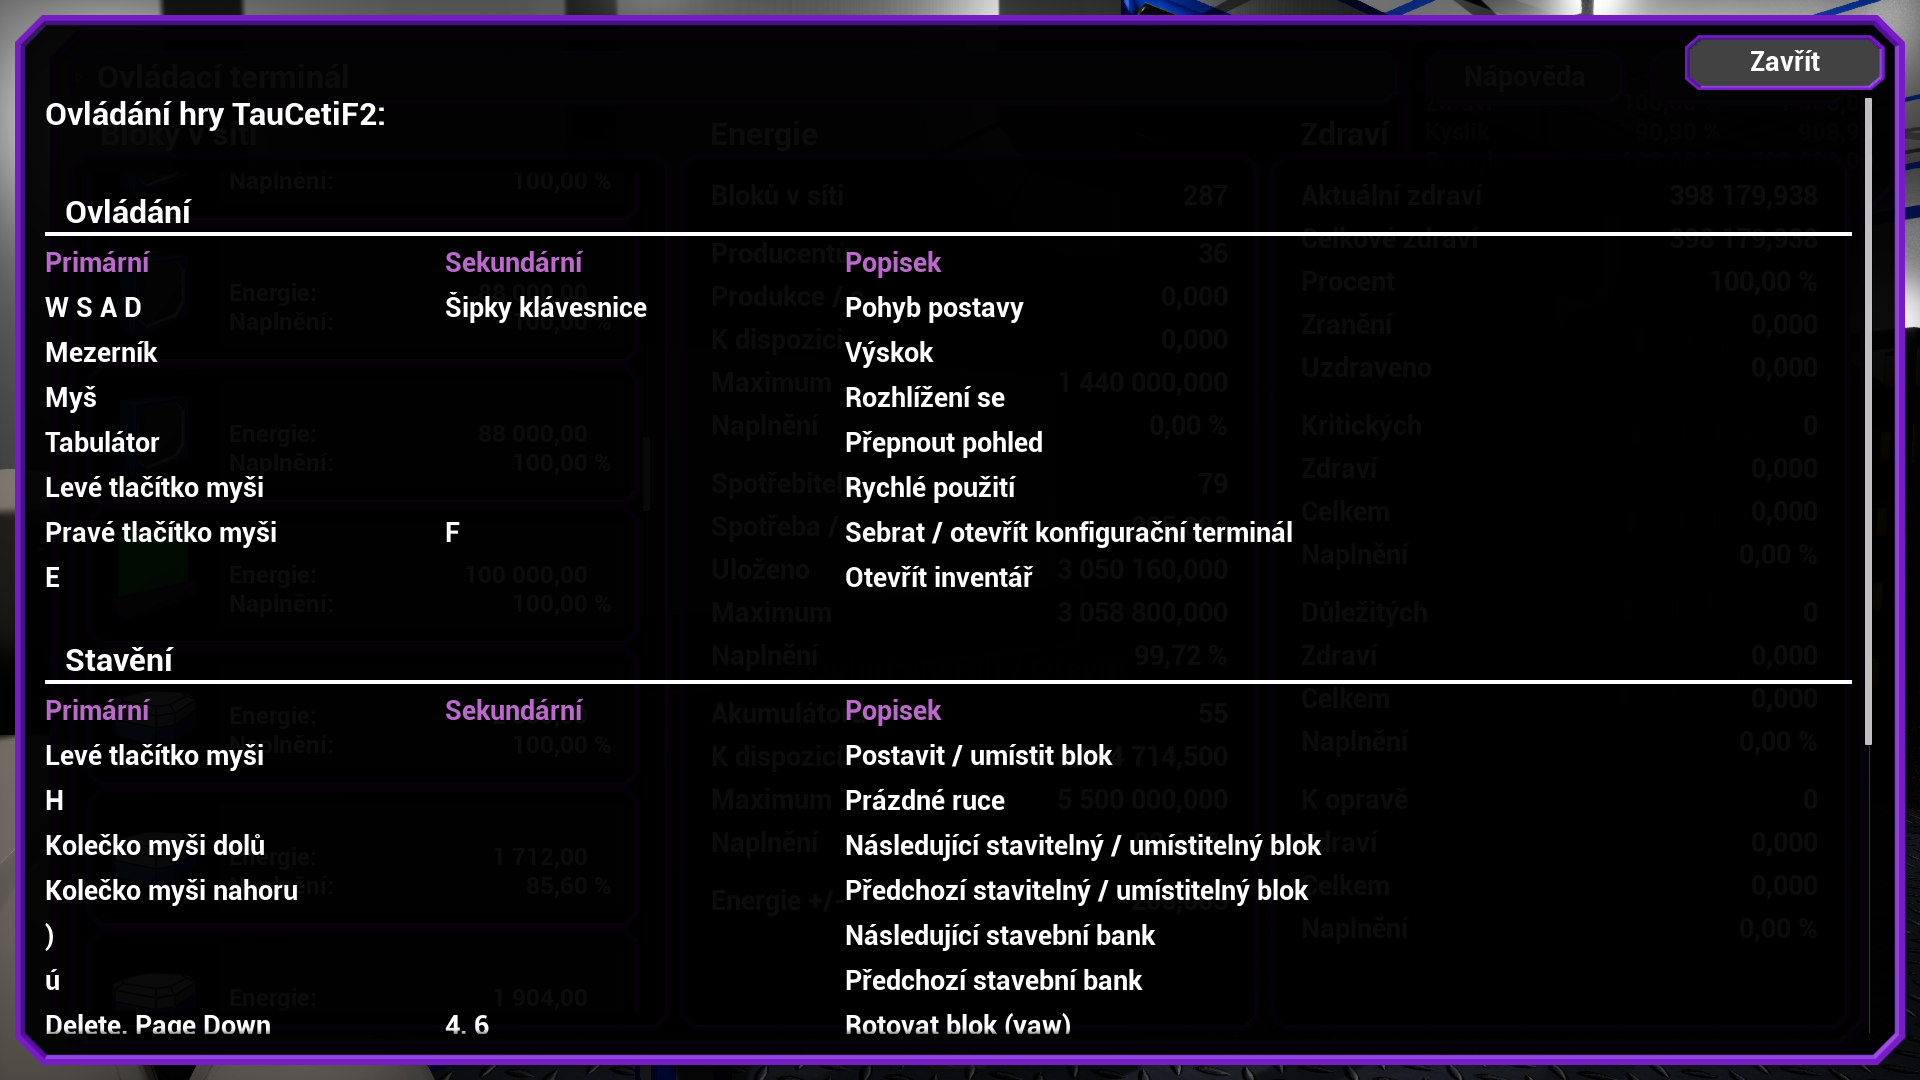
\includegraphics[ width=140mm]{../img/user/terminal/2terminalHelp}

\caption{Terminál - nápověda}
\label{fig:user_terminal_2terminalHelp}

\end{figure}

\FloatBarrier

Selektor dostupných obrazovek:

\begin{figure}[!h]\centering
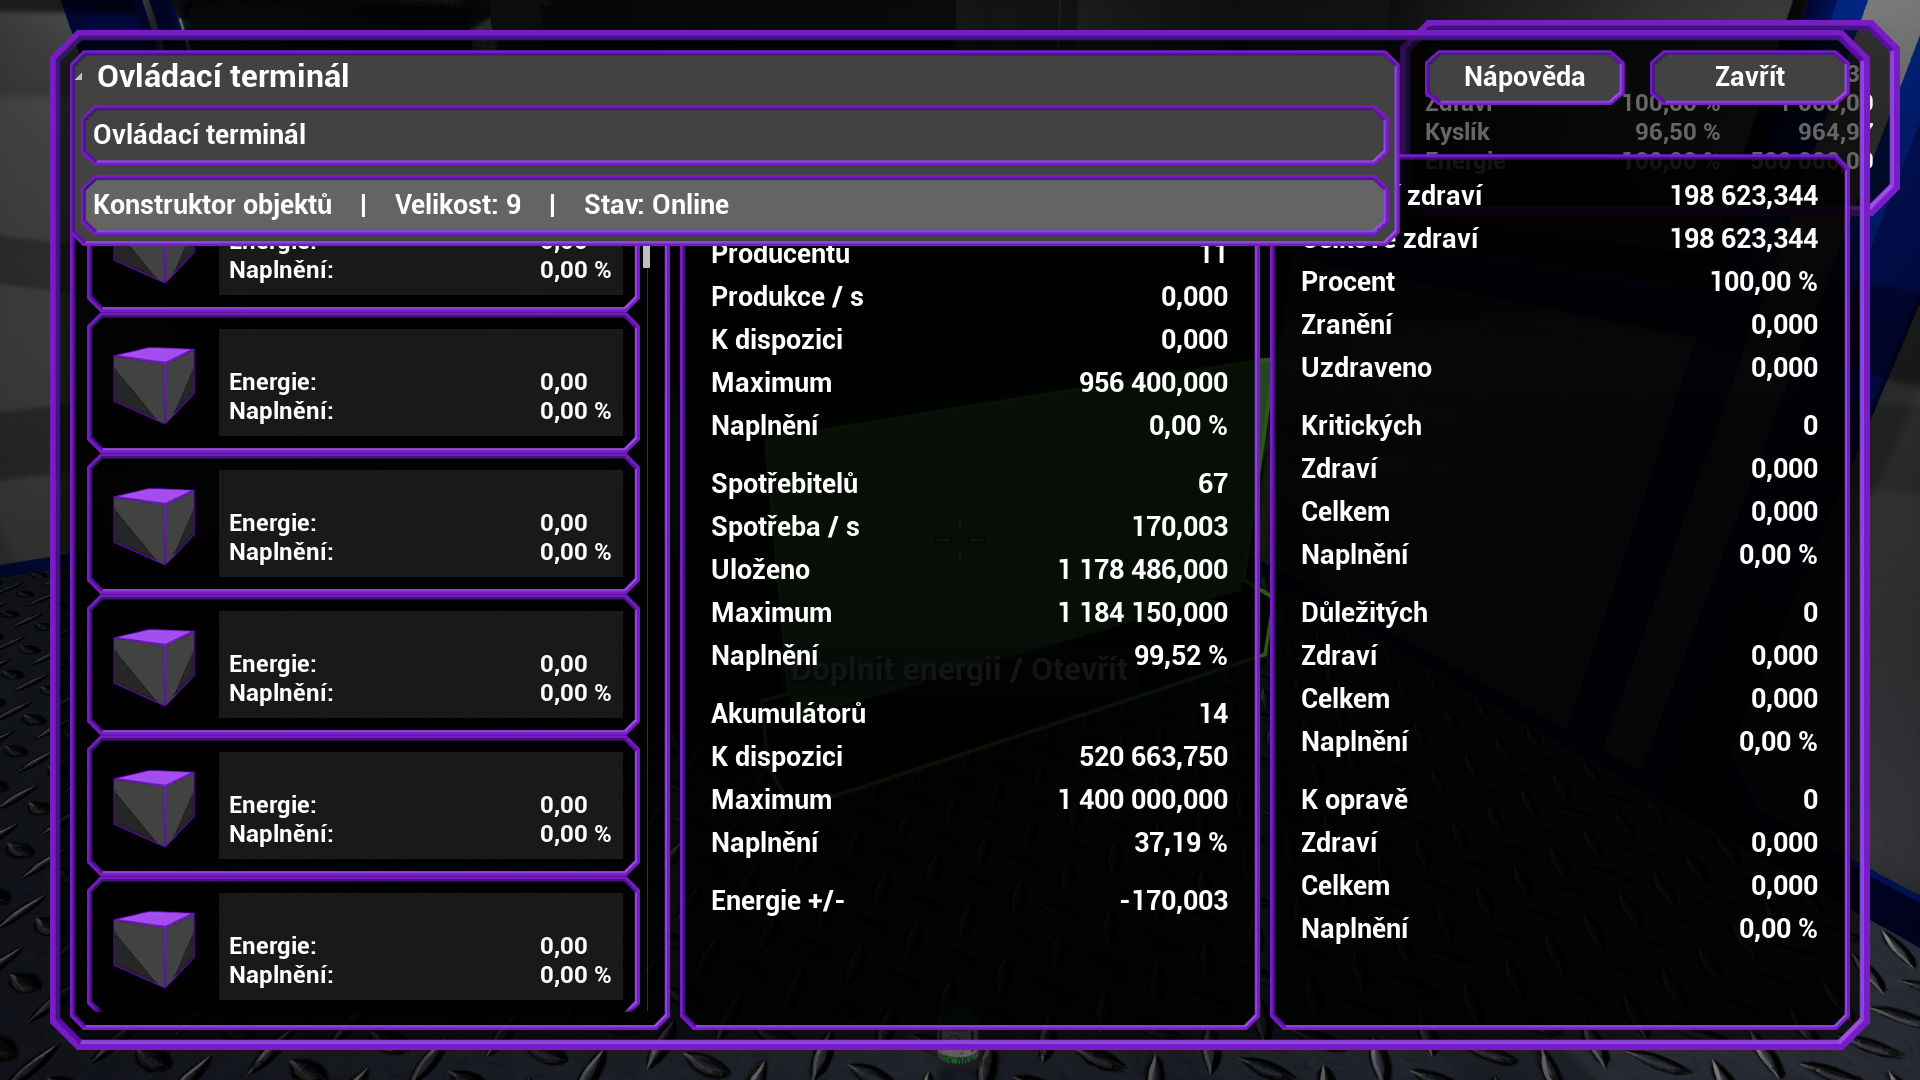
\includegraphics[ width=140mm]{../img/user/terminal/3terminalCtorSelector}

\caption{Terminál - selektor obrazovek}
\label{fig:user_terminal_3terminalCtorSelector}

\end{figure}

\FloatBarrier

Pokud vybereme \textbf{Konstruktor objektů}, vidíme seznam dostupných bloků, které můžeme zkonstruovat. Pokud to pro některé nelze (třeba z důvodu omezení velikosti - konstruktor je na daný objekt příliš malý), blok není aktivní a nelze ho zvolit.


\begin{figure}[!h]\centering
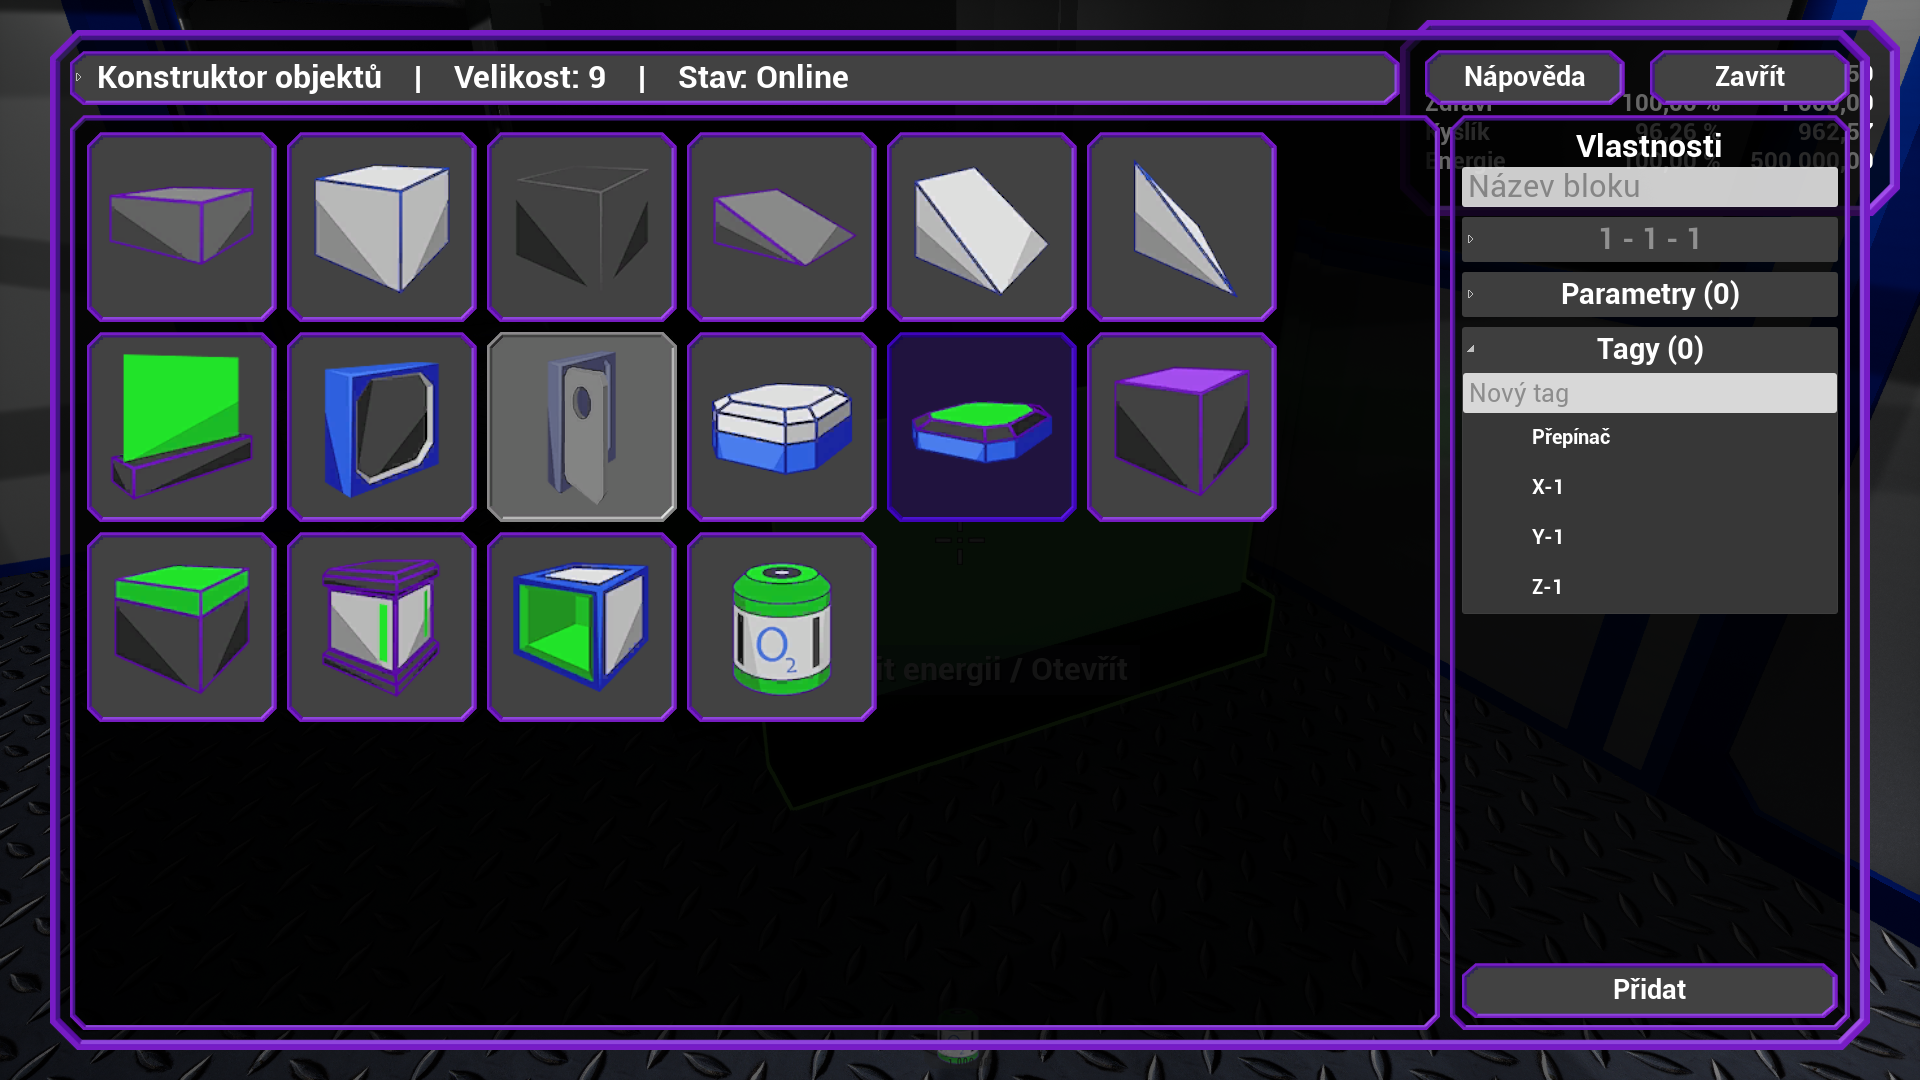
\includegraphics[ width=140mm]{../img/user/terminal/4builderSmall}

\caption{Terminál - konstruktor objektů}
\label{fig:user_terminal_4builderSmall}

\end{figure}

\FloatBarrier

V sekci \textit{Nastavení} je možné kromě tagů definovat i požadovanou velikost a to až do velikosti konstruktoru, nebo globálního omezení 20 násobku  základní kostky.

\begin{figure}[!h]\centering
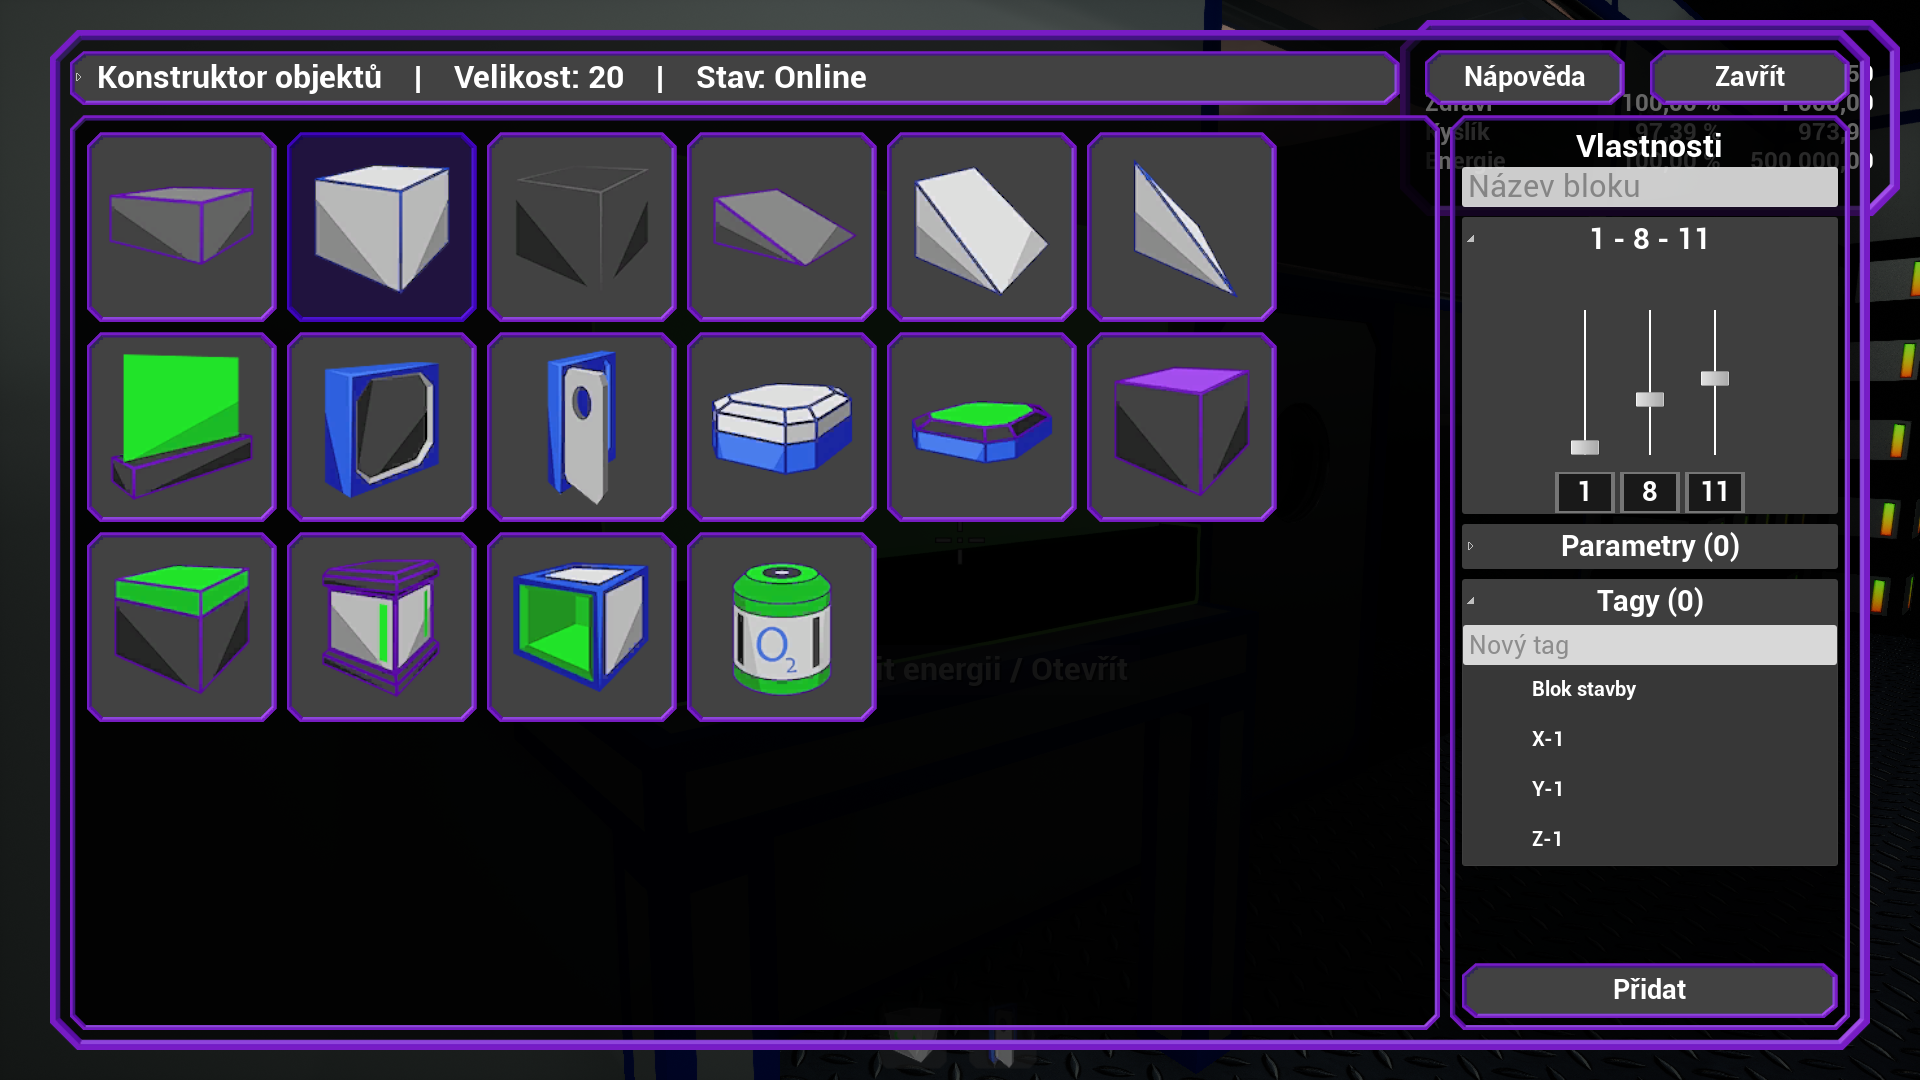
\includegraphics[ width=140mm]{../img/user/terminal/5builderSize}

\caption{Terminál - Nastavení velikosti}
\label{fig:user_terminal_5builderSize}

\end{figure}

\FloatBarrier

Některé bloky, třeba \textbf{Dveře} požadují dodatečné parametry, které ovlivňují jejich výsledné chování. V našem případě to je smysl otevírání dveří při čelním pohledu. Na obrázku je vidět stav po rozkliknutí.

\begin{figure}[!h]\centering
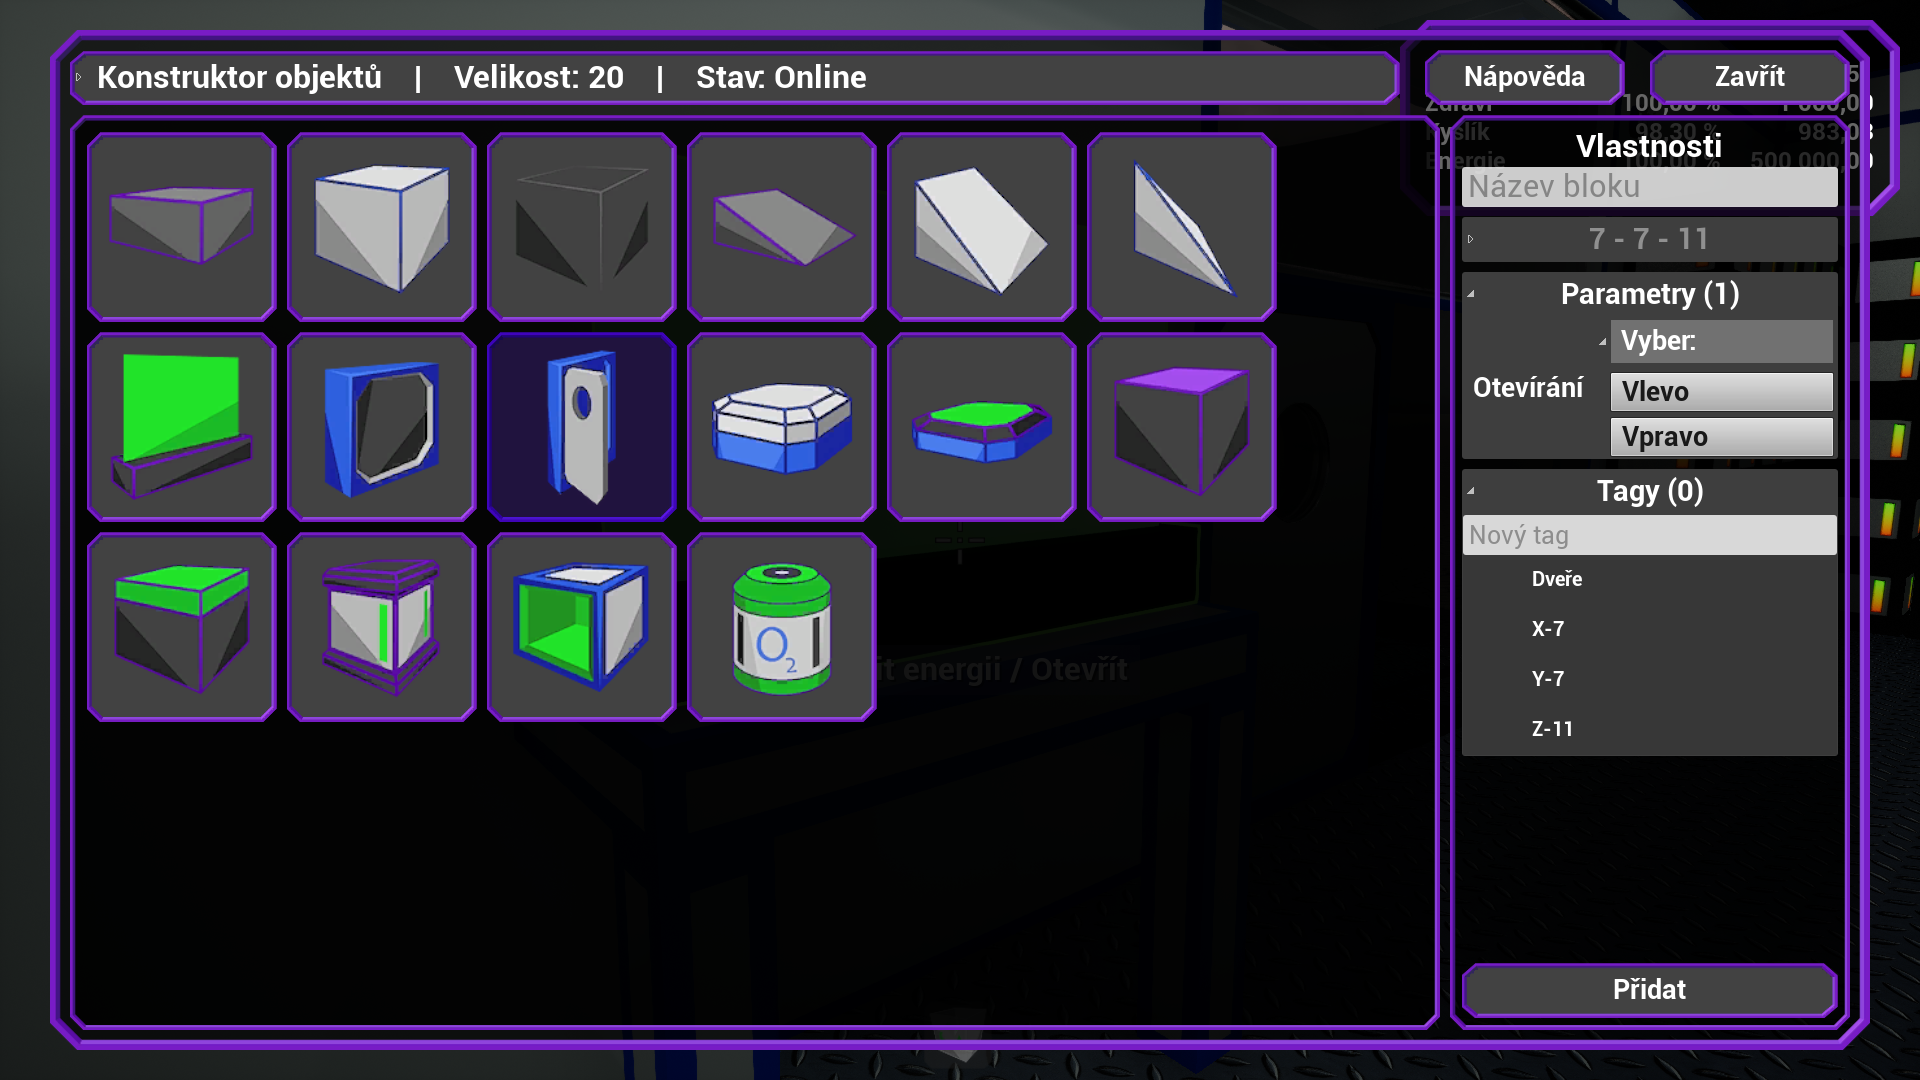
\includegraphics[ width=140mm]{../img/user/terminal/6builderParams}

\caption{Terminál - Nastavení parametrů}
\label{fig:user_terminal_6builderParams}

\end{figure}

\FloatBarrier
%%!TEX root = ../../prace.tex

\section{Stavební akce}

\textbf{Destruktor} umožňuje mazat bloky. Po jeho výběru je vidět červený outline vybraného bloku.

\begin{figure}[!ht]\centering
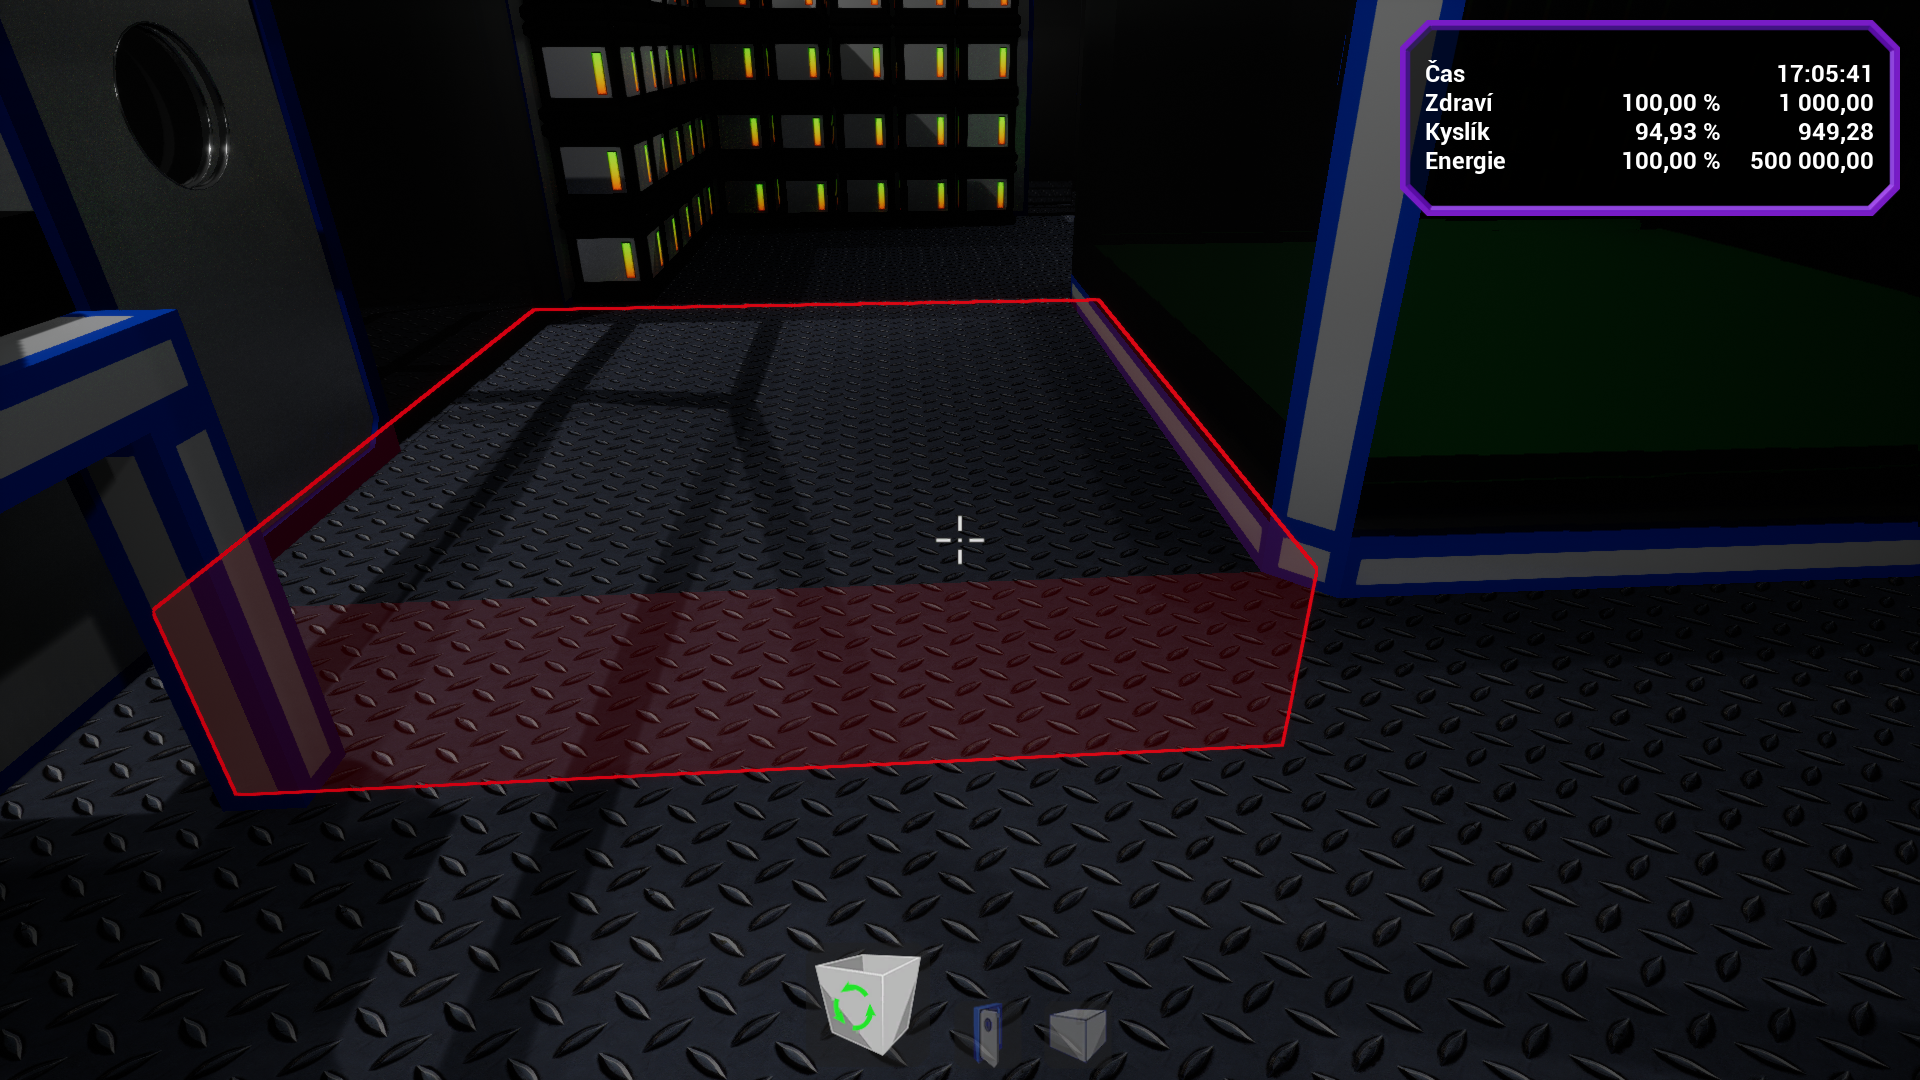
\includegraphics[ width=140mm]{../img/user/buildActions/delete}

\caption{Stavění -- smazat}
\label{fig:user_buildActions_delete}

\end{figure}

\FloatBarrier

Pokud vybereme umístění nového bloku, vidíme žlutě hranice sousedního bloku, ke kterému blok přistavujeme. Stavěný / umisťovaný blok musí mít dostatečné místo pro svoje umístění. Dále je potřeba mít s~sebou dostatečně velkou zásobu energie (dle energetické náročnosti bloku).

\begin{figure}[!ht]\centering
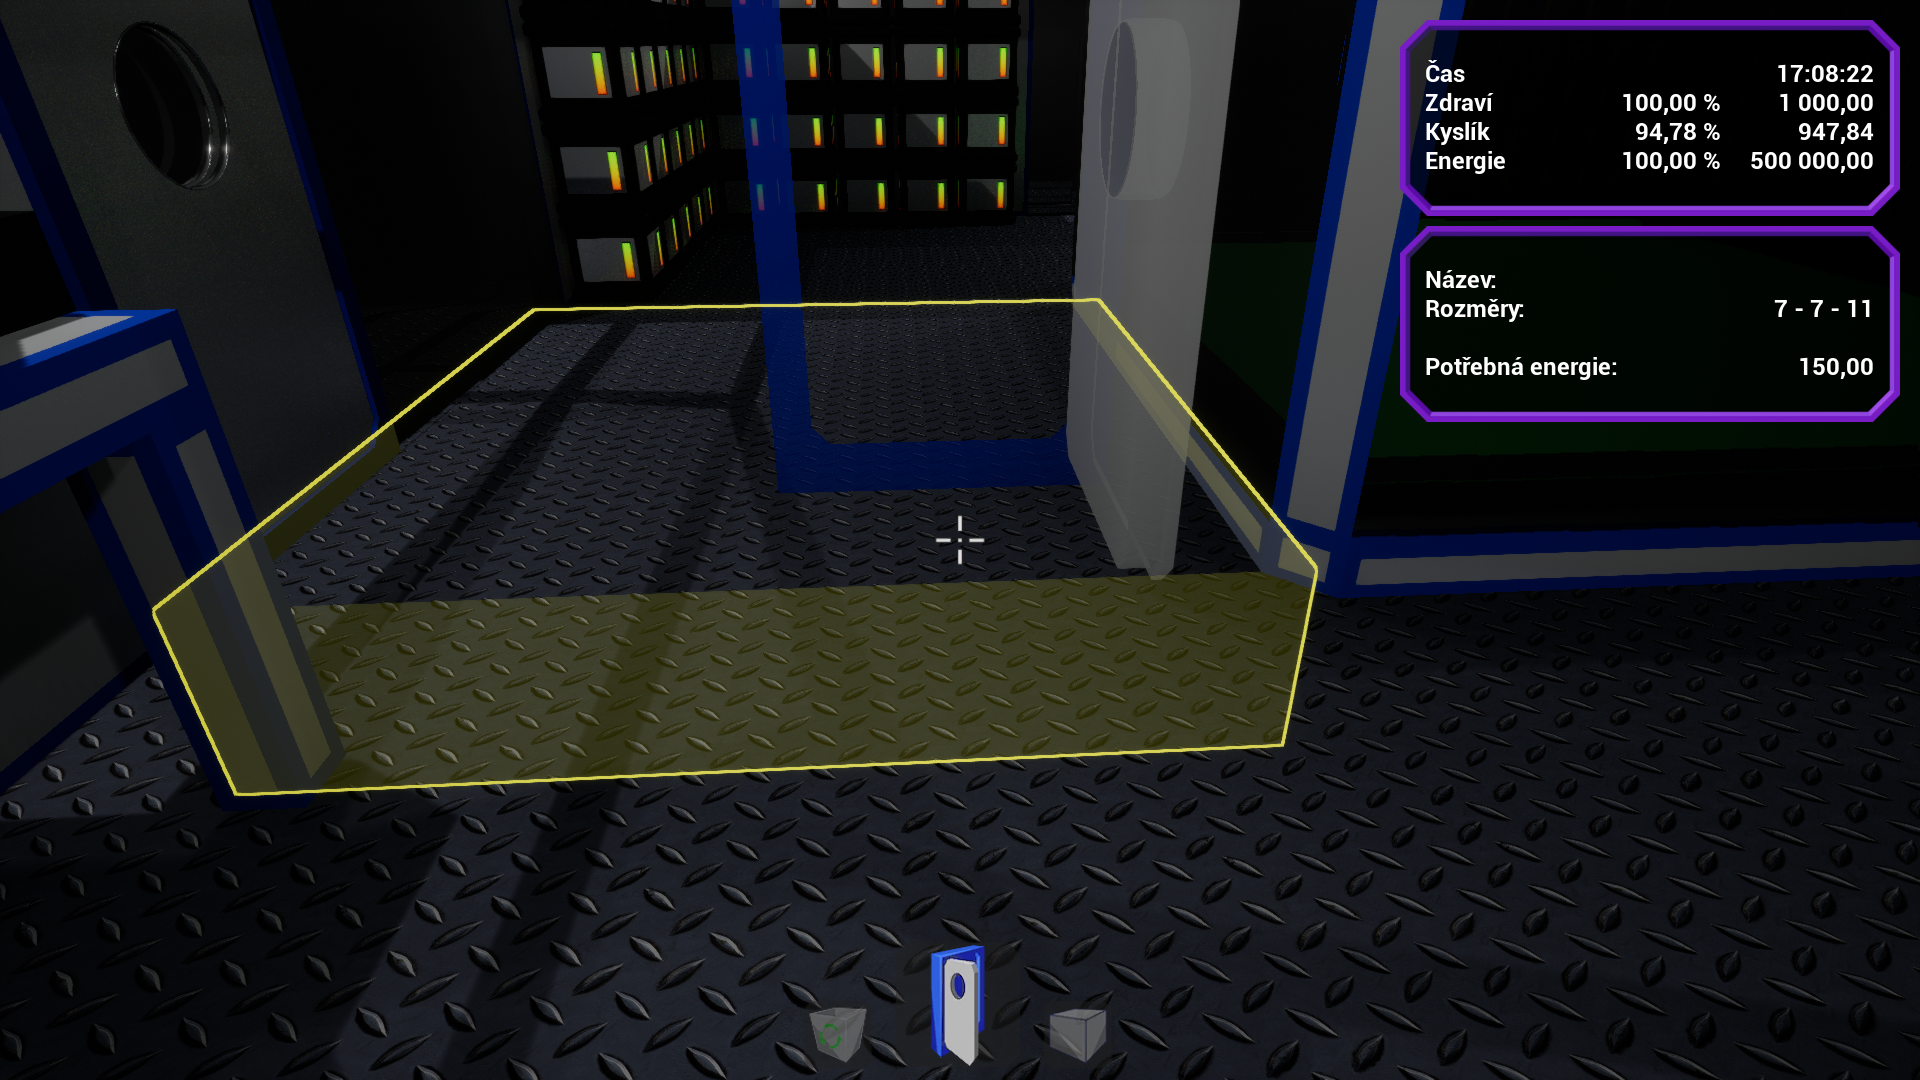
\includegraphics[ width=140mm]{../img/user/buildActions/place}

\caption{Stavění -- umístit}
\label{fig:user_buildActions_place}

\end{figure}

\FloatBarrier

Blok je též možný rotovat (Klávesy v~sekci Insert .. Page Down, případně jejich ekvivalenty 7,8,9,4,5,6).

\begin{figure}[!ht]\centering
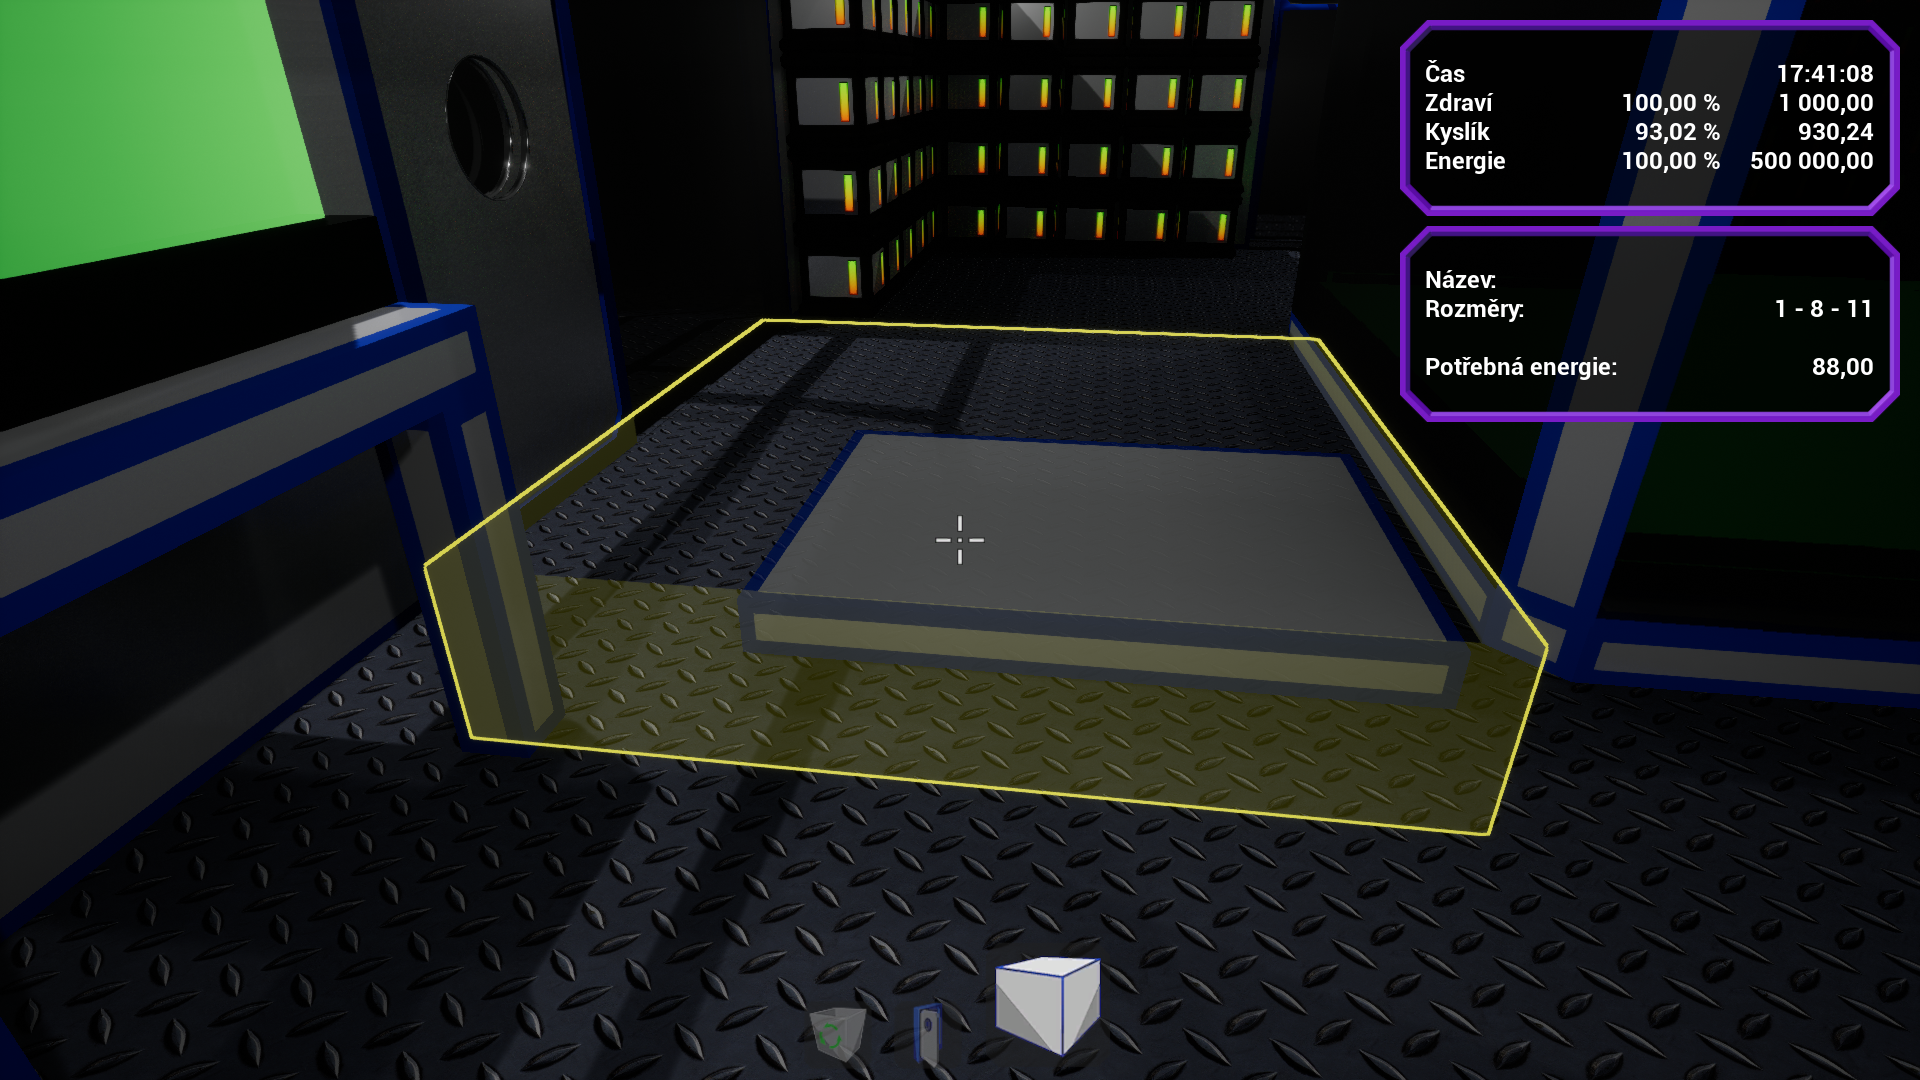
\includegraphics[ width=140mm]{../img/user/buildActions/place_Rotate}

\caption{Stavění -- rotace}
\label{fig:user_buildActions_place_Rotate}

\end{figure}

\FloatBarrier

Pokud bylo umístění v~pořádku, blok již není nadále průhledný a~hráči ubyla energie. Pokud je zapnut kreativní mód, energie samozřejmě neubývá.

\begin{figure}[!ht]\centering
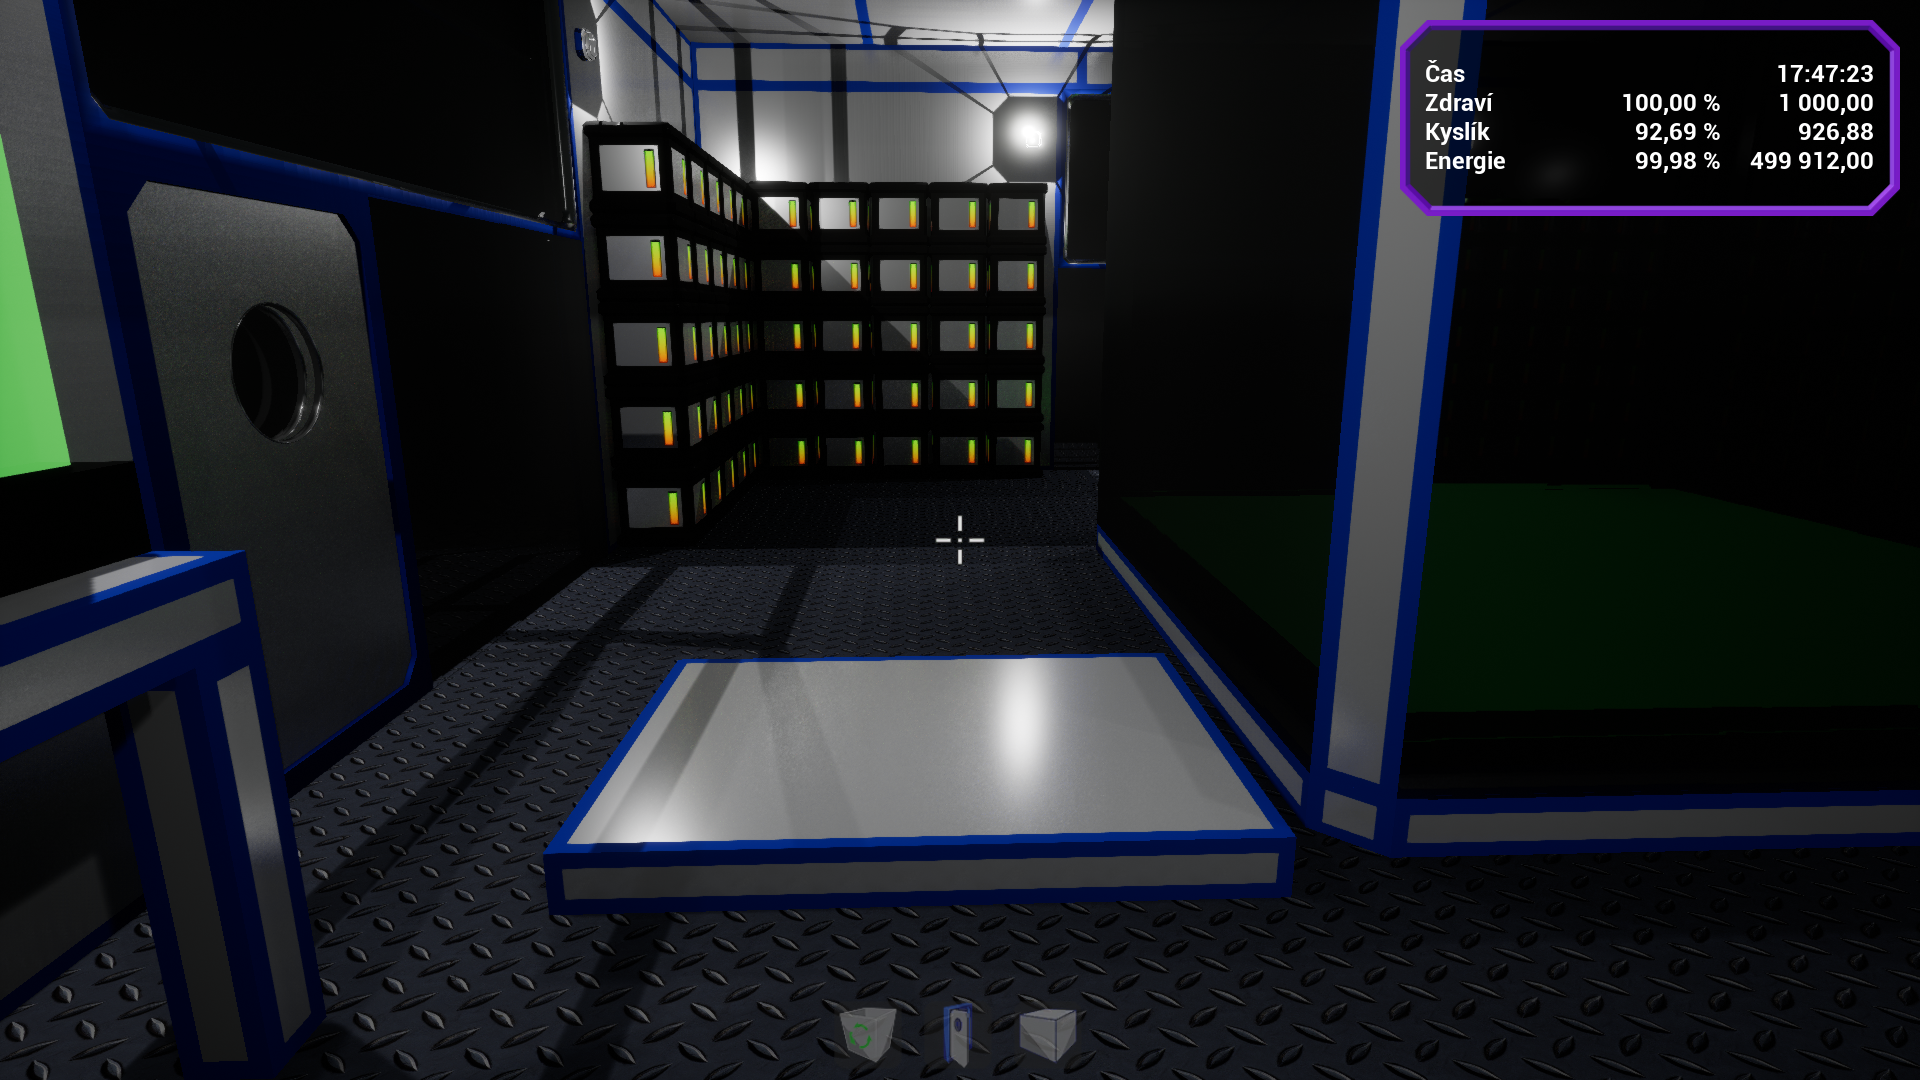
\includegraphics[ width=140mm]{../img/user/buildActions/placeAfter}

\caption{Stavění -- po umístění}
\label{fig:user_buildActions_placeAfter}

\end{figure}


\FloatBarrier
%%!TEX root = ../../prace.tex

\section{Umístitelné předměty}

Blok \textbf{Kyslíková bomba} je možné umístit do světa a pak si ho opět vzít do inventáře. Díky tomu je možné tyto bloky dále používat třeba pro plnění v \textbf{Plničce kyslíkových bomb}.
Blok je možné buď rovnou použít (levé tlačítko myši).
Tento blok zároveň rovnou ukazuje, kolik objemu je využito.

\begin{figure}[!ht]\centering
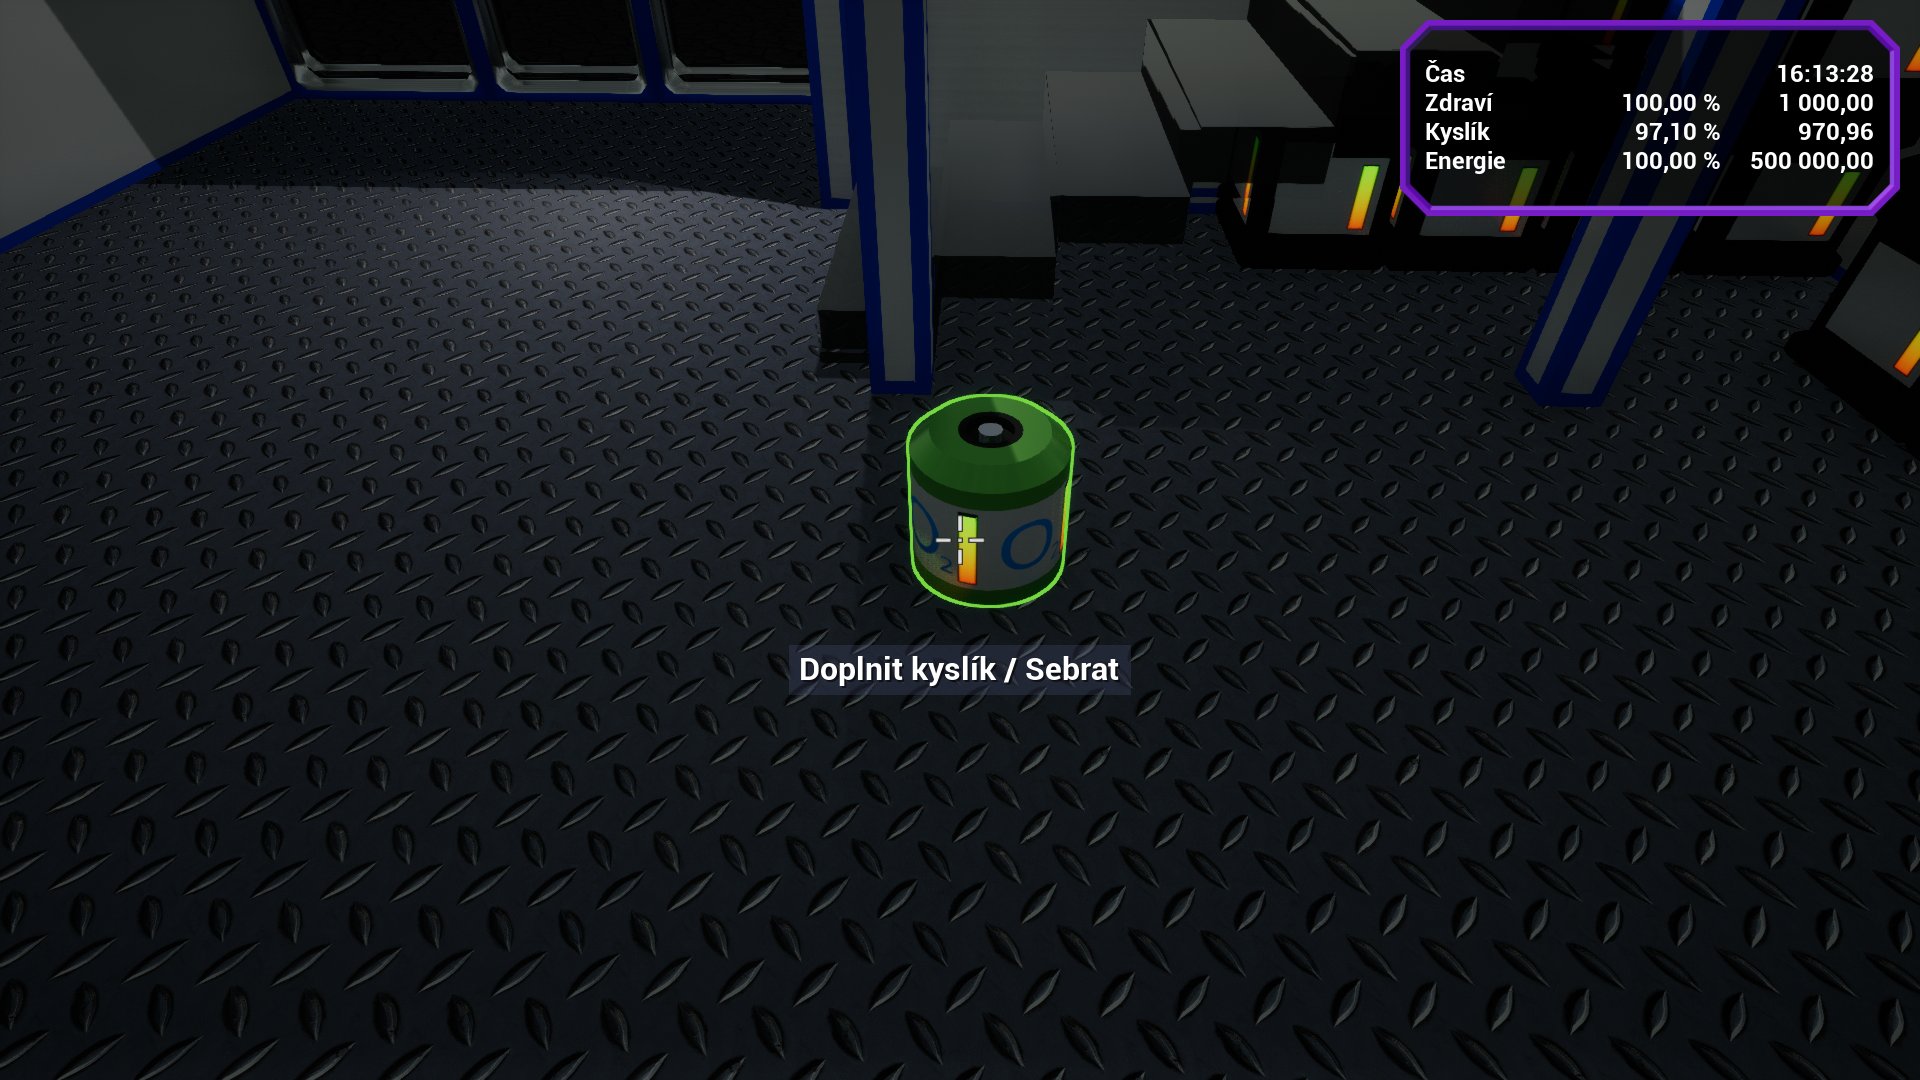
\includegraphics[ width=140mm]{../../img/user/tank/0tankFull}

\caption{Umístitelné předměty - plná kyslíková bomba}
\label{fig:user_tank_0tankFull}

\end{figure}

\FloatBarrier

Na dalším obrázku vidíme již částečně použitou kyslíkovou bombu. Pokud ji pravým tlačítkem myši sebereme a otevřeme si inventář a správnou skupinu (\textbf{Typ: Inventář} v nastavení skupiny), uvidíme tento blok v seznamu.

Požité tagy se při přidání do světa a opětovném sebrání zachovávají.

\begin{figure}[!ht]\centering
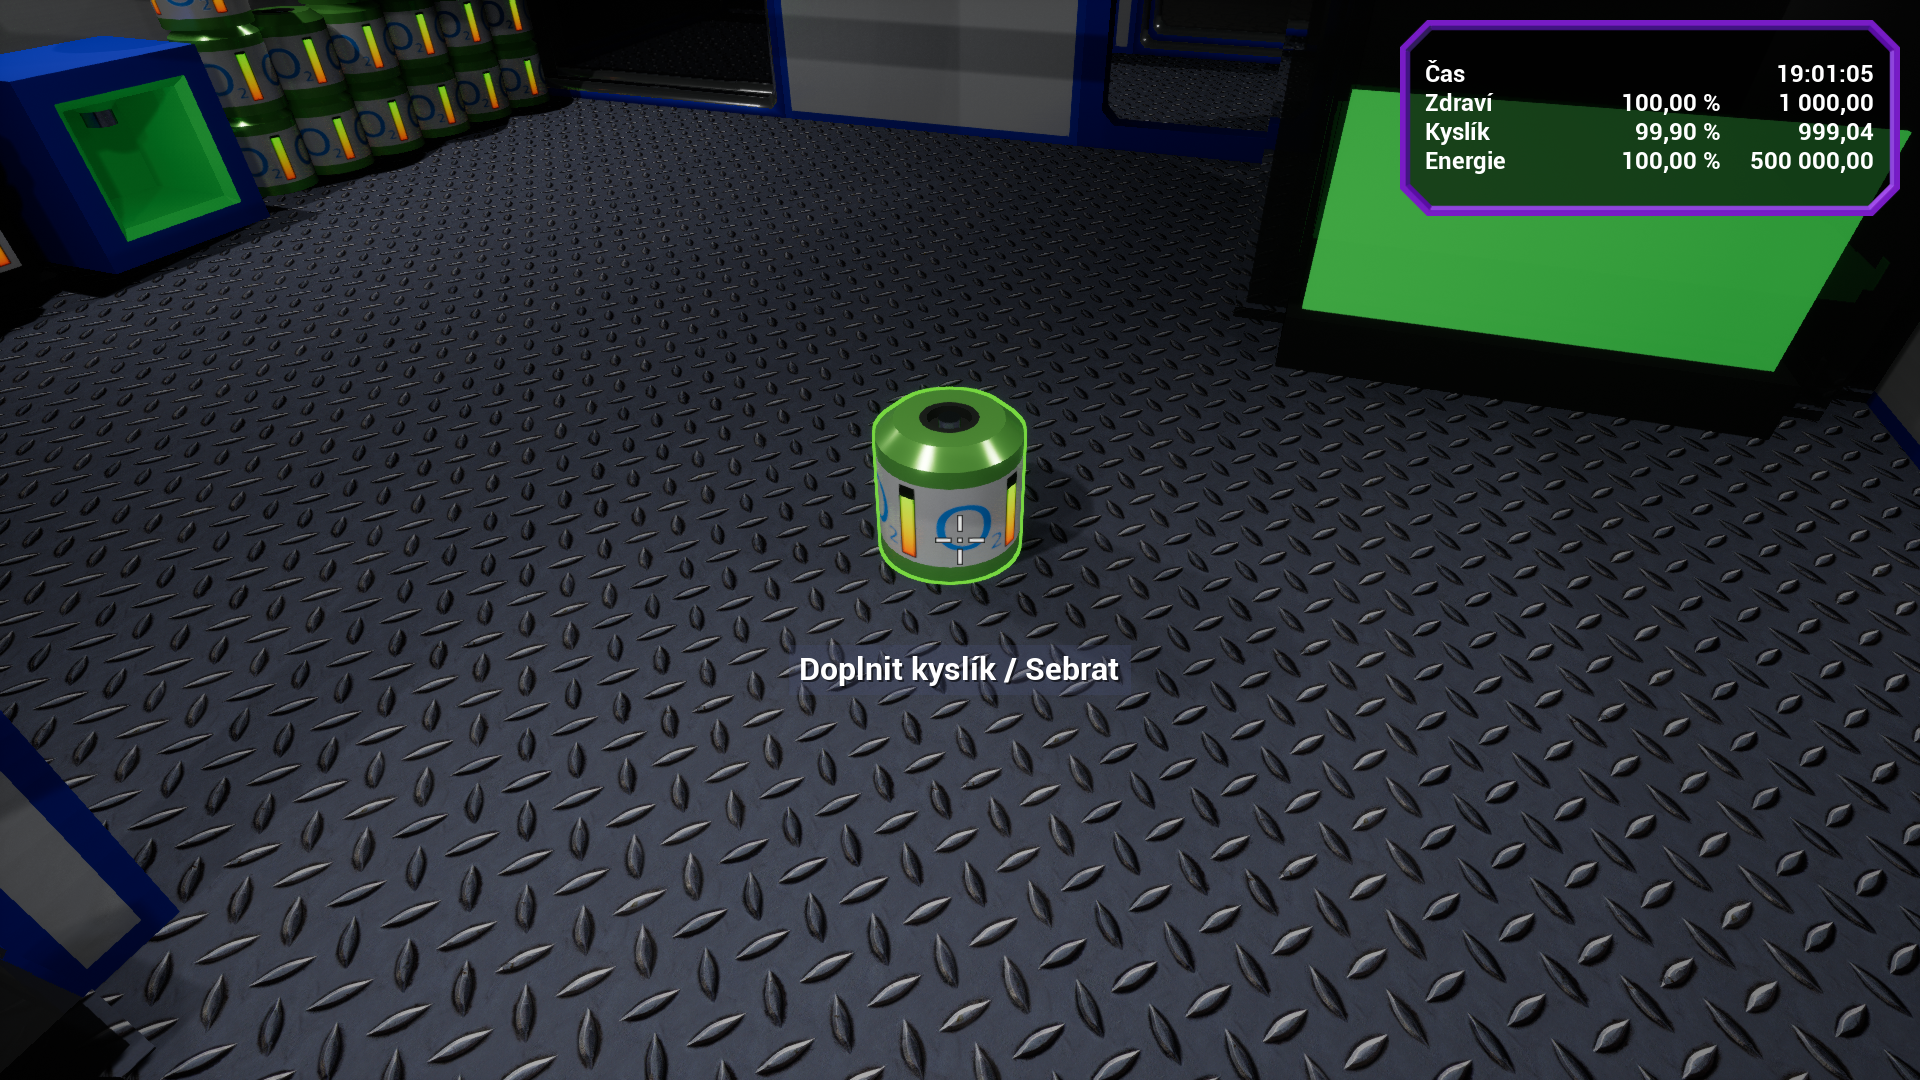
\includegraphics[ width=140mm]{../../img/user/tank/1tankAfterUse}

\caption{Umístitelné předměty - použitá bomba}
\label{fig:user_tank_1tankAfterUse}

\end{figure}

\FloatBarrier

Zároveň v inventáři můžeme vidět přesnou hodnotu naplnění bloku.

\begin{figure}[!ht]\centering
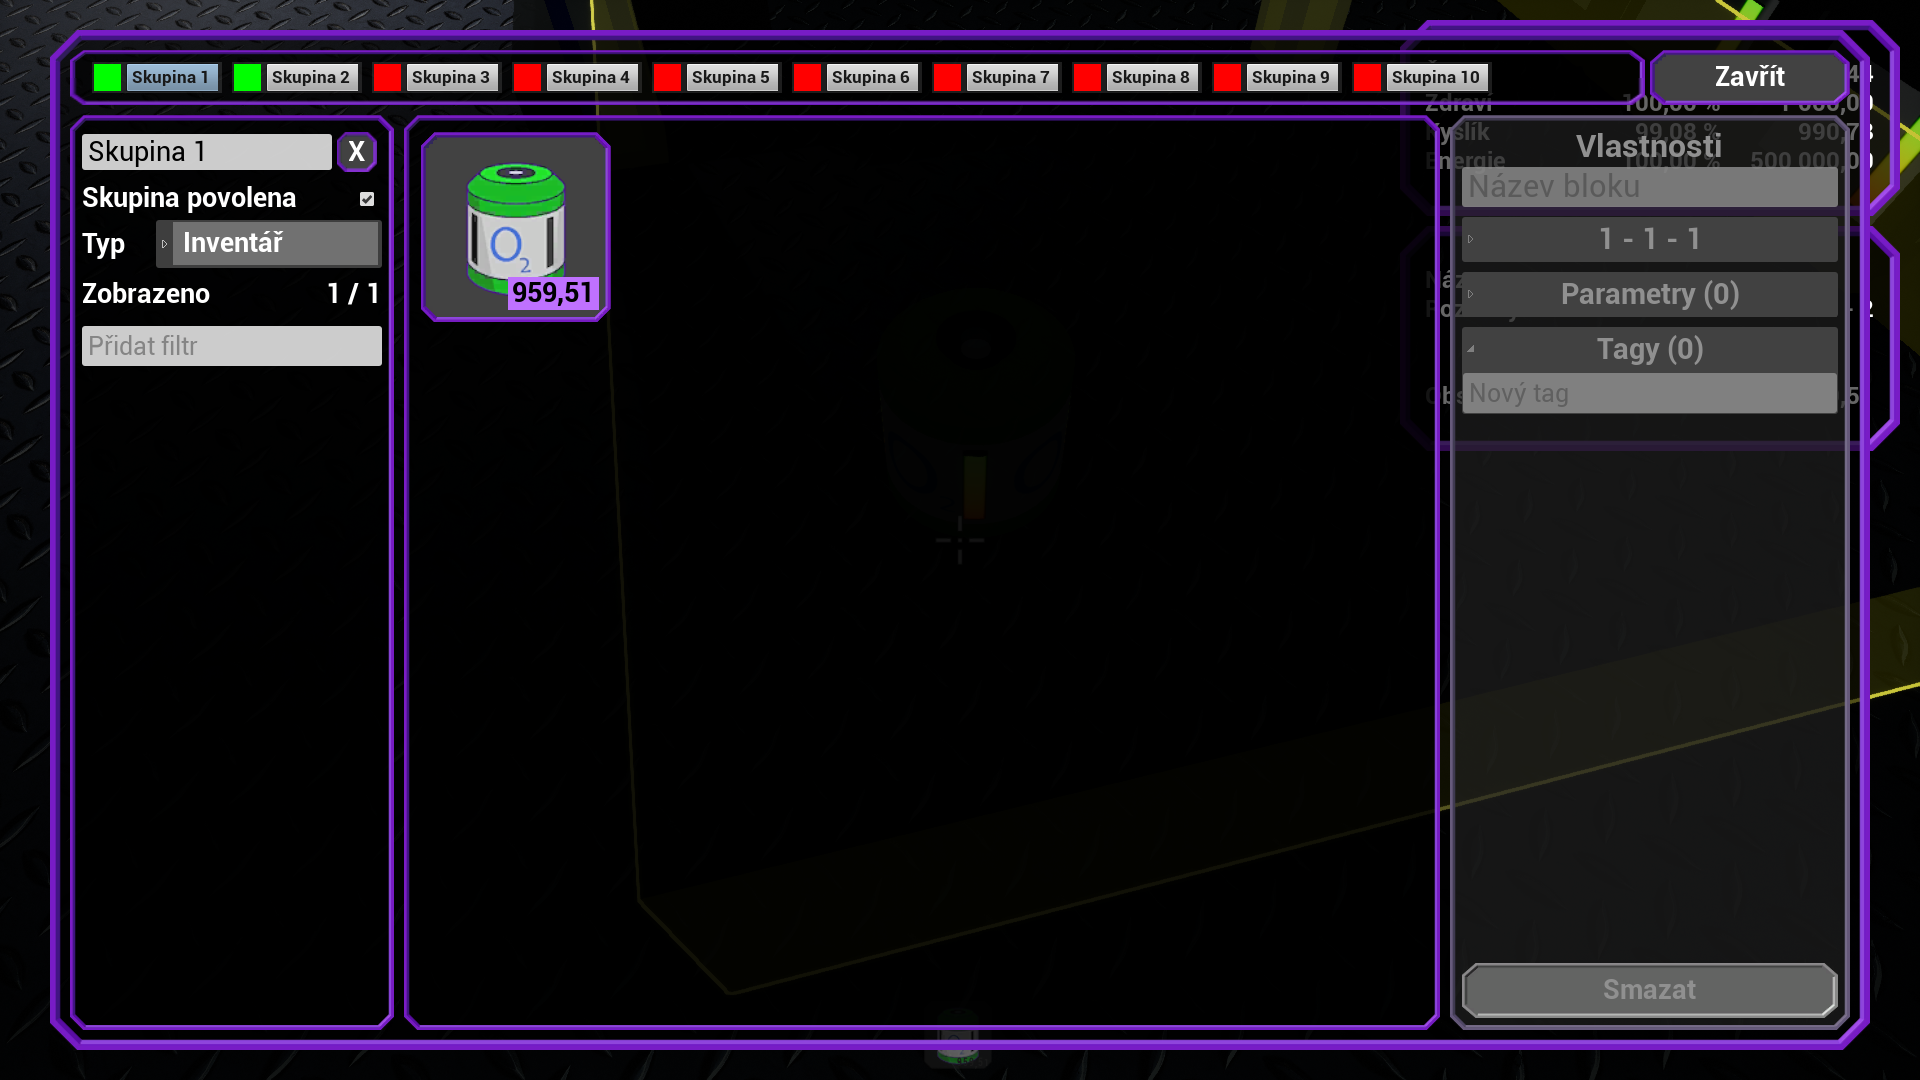
\includegraphics[ width=140mm]{../../img/user/tank/2tankInventory}

\caption{Umístitelné předměty - inventář}
\label{fig:user_tank_2tankInventory}

\end{figure}



\FloatBarrier
%%!TEX root = ../../prace.tex

\section{Plnička kyslíkových bomb}

Kyslíkové bomby je potřeba opětovně naplnit, pokud byl jejich obsah spotřebován. Stejně jako u~Kyslíkové bomby, levým tlačítkem myši je možné rovnou doplnit zásoby kyslíku hráče. Pravým se pak otevře ovládací obrazovka.

\begin{figure}[!ht]\centering
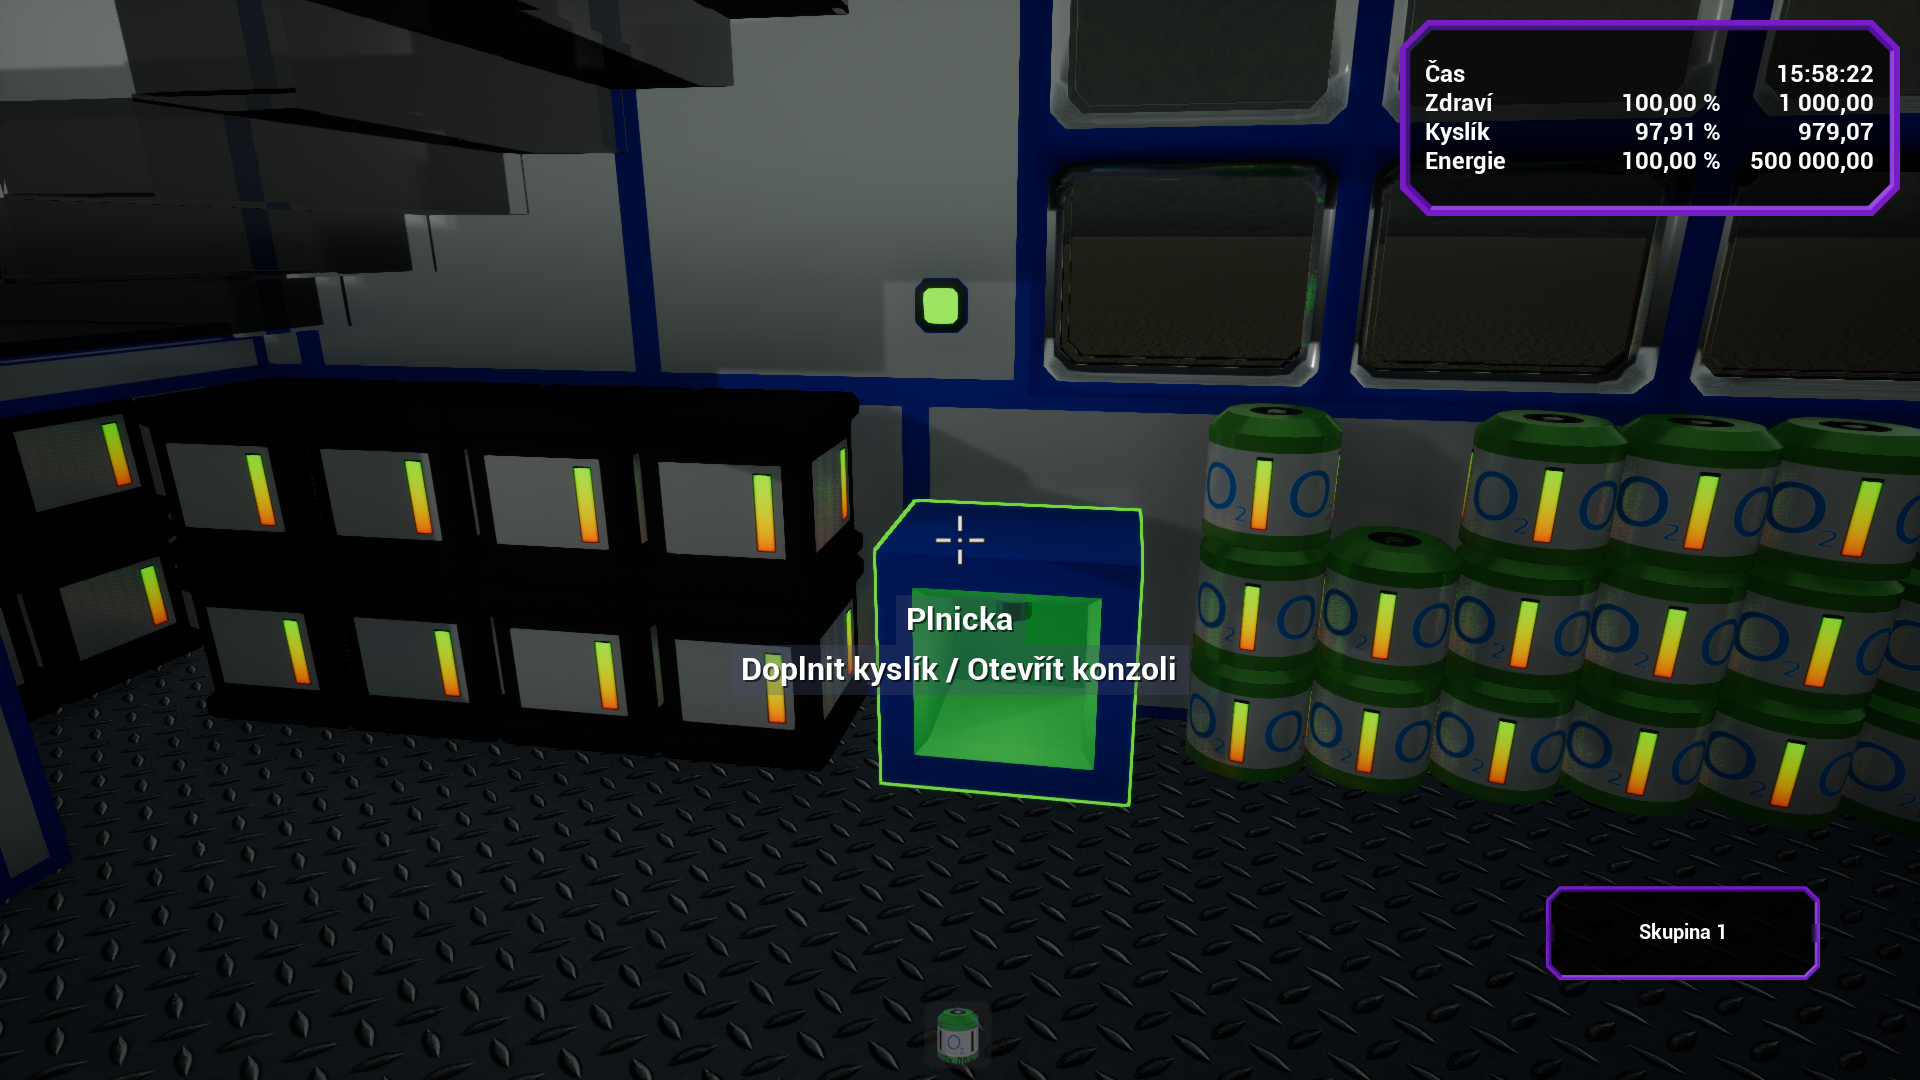
\includegraphics[ width=140mm]{../img/user/filler/0use}

\caption{Plnička kyslíkové bomby -- náhled}
\label{fig:user_filler_0use}

\end{figure}

\FloatBarrier

Ta má v~levé části přiřazený ovladač, případně je možné nejvýše jeden ovladač ze seznamu ovladačů přiřadit. Pokud je přiřazen ovladač, zapnutí bloku se řídí jeho nastavením. V~pravé části je možné regulovat spotřebovávanou energii.

Uprostřed je možné vybrat bomby, které jsou v~inventáři hráče, k~naplnění.

\begin{figure}[!ht]\centering
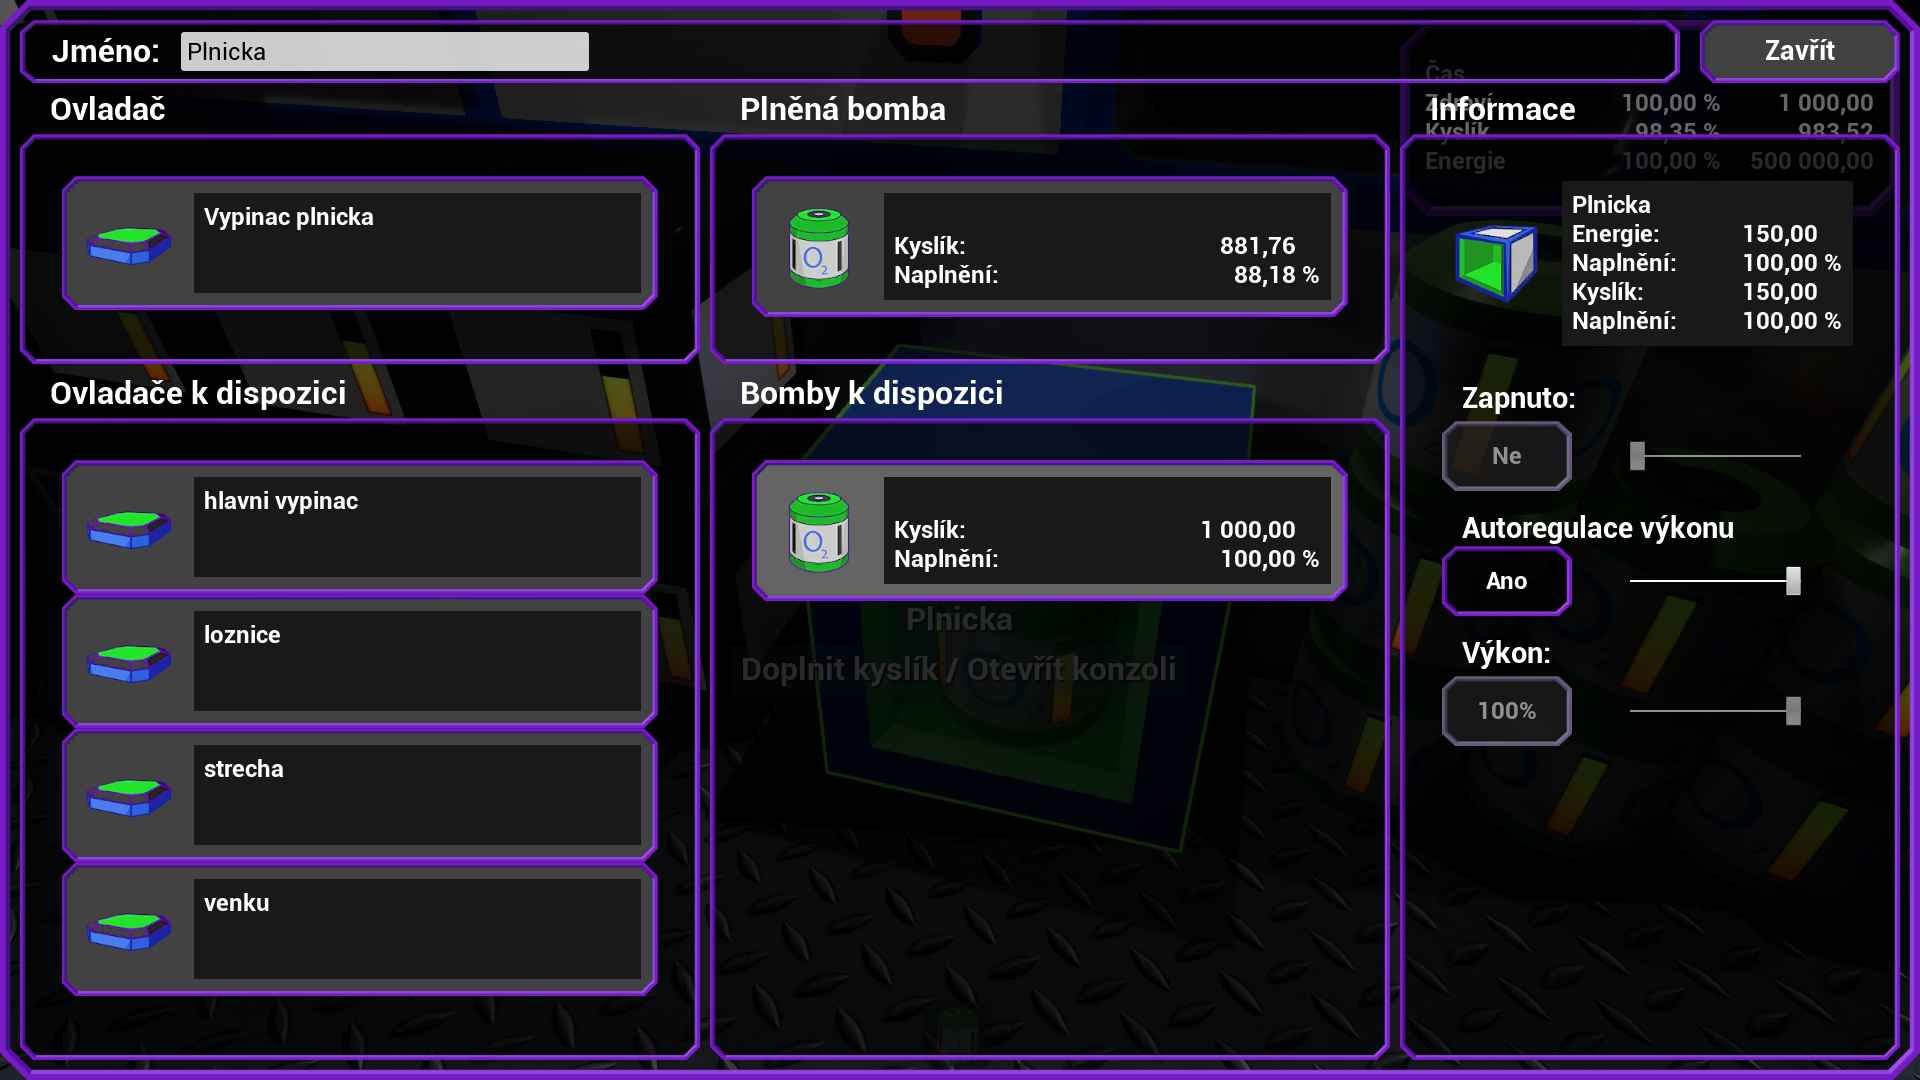
\includegraphics[ width=140mm]{../img/user/filler/1fill}

\caption{Plnička kyslíkové bomby -- ovládací obrazovka}
\label{fig:user_filler_1fill}

\end{figure}

\FloatBarrier

Pokud je plnička zapnuta, generuje kyslík a~ze své zásoby plní přiřazenou kyslíkovou bombu.

\begin{figure}[!ht]\centering
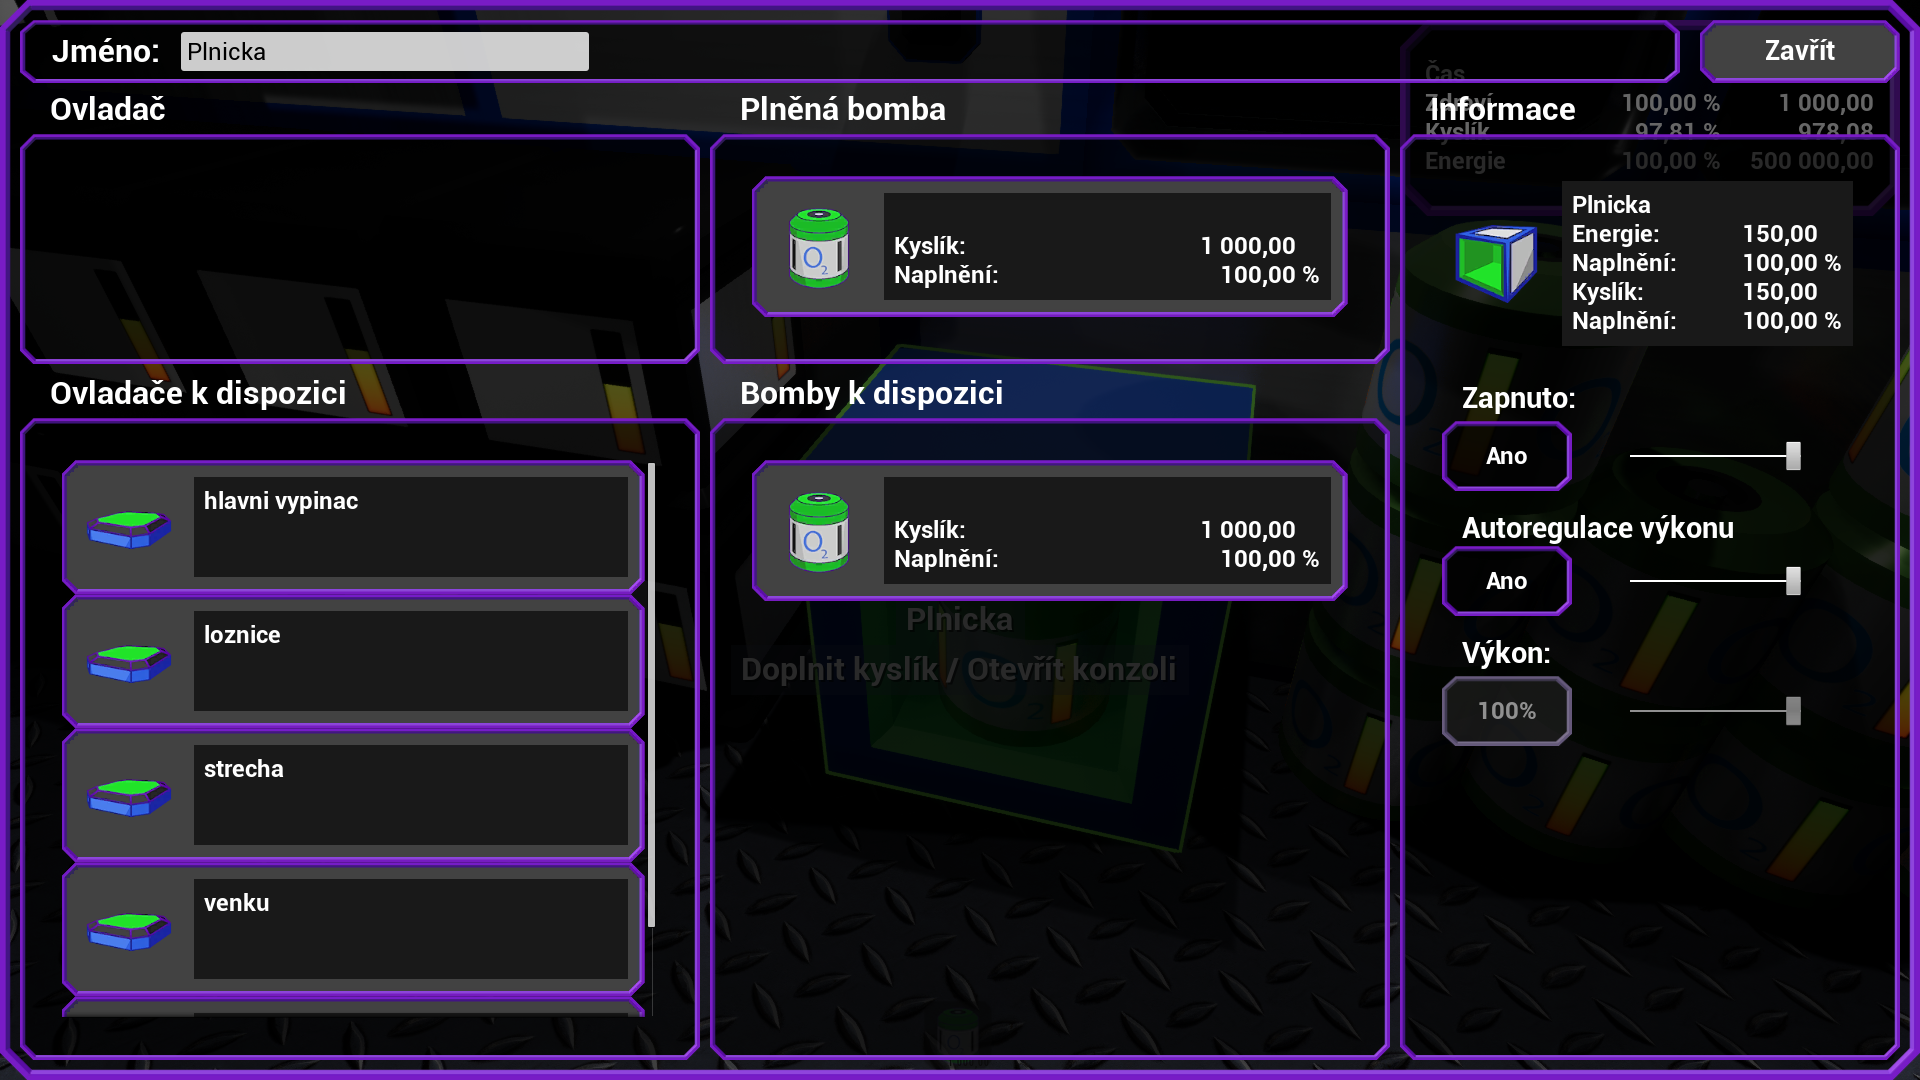
\includegraphics[ width=140mm]{../img/user/filler/2filled}

\caption{Plnička kyslíkové bomby -- naplněno}
\label{fig:user_filler_2filled}

\end{figure}



\FloatBarrier
%%!TEX root = ../prace.tex

\section{Přepínač}

Přepínač slouží jako ovládání pro světla a plničku

\begin{figure}[!h]\centering
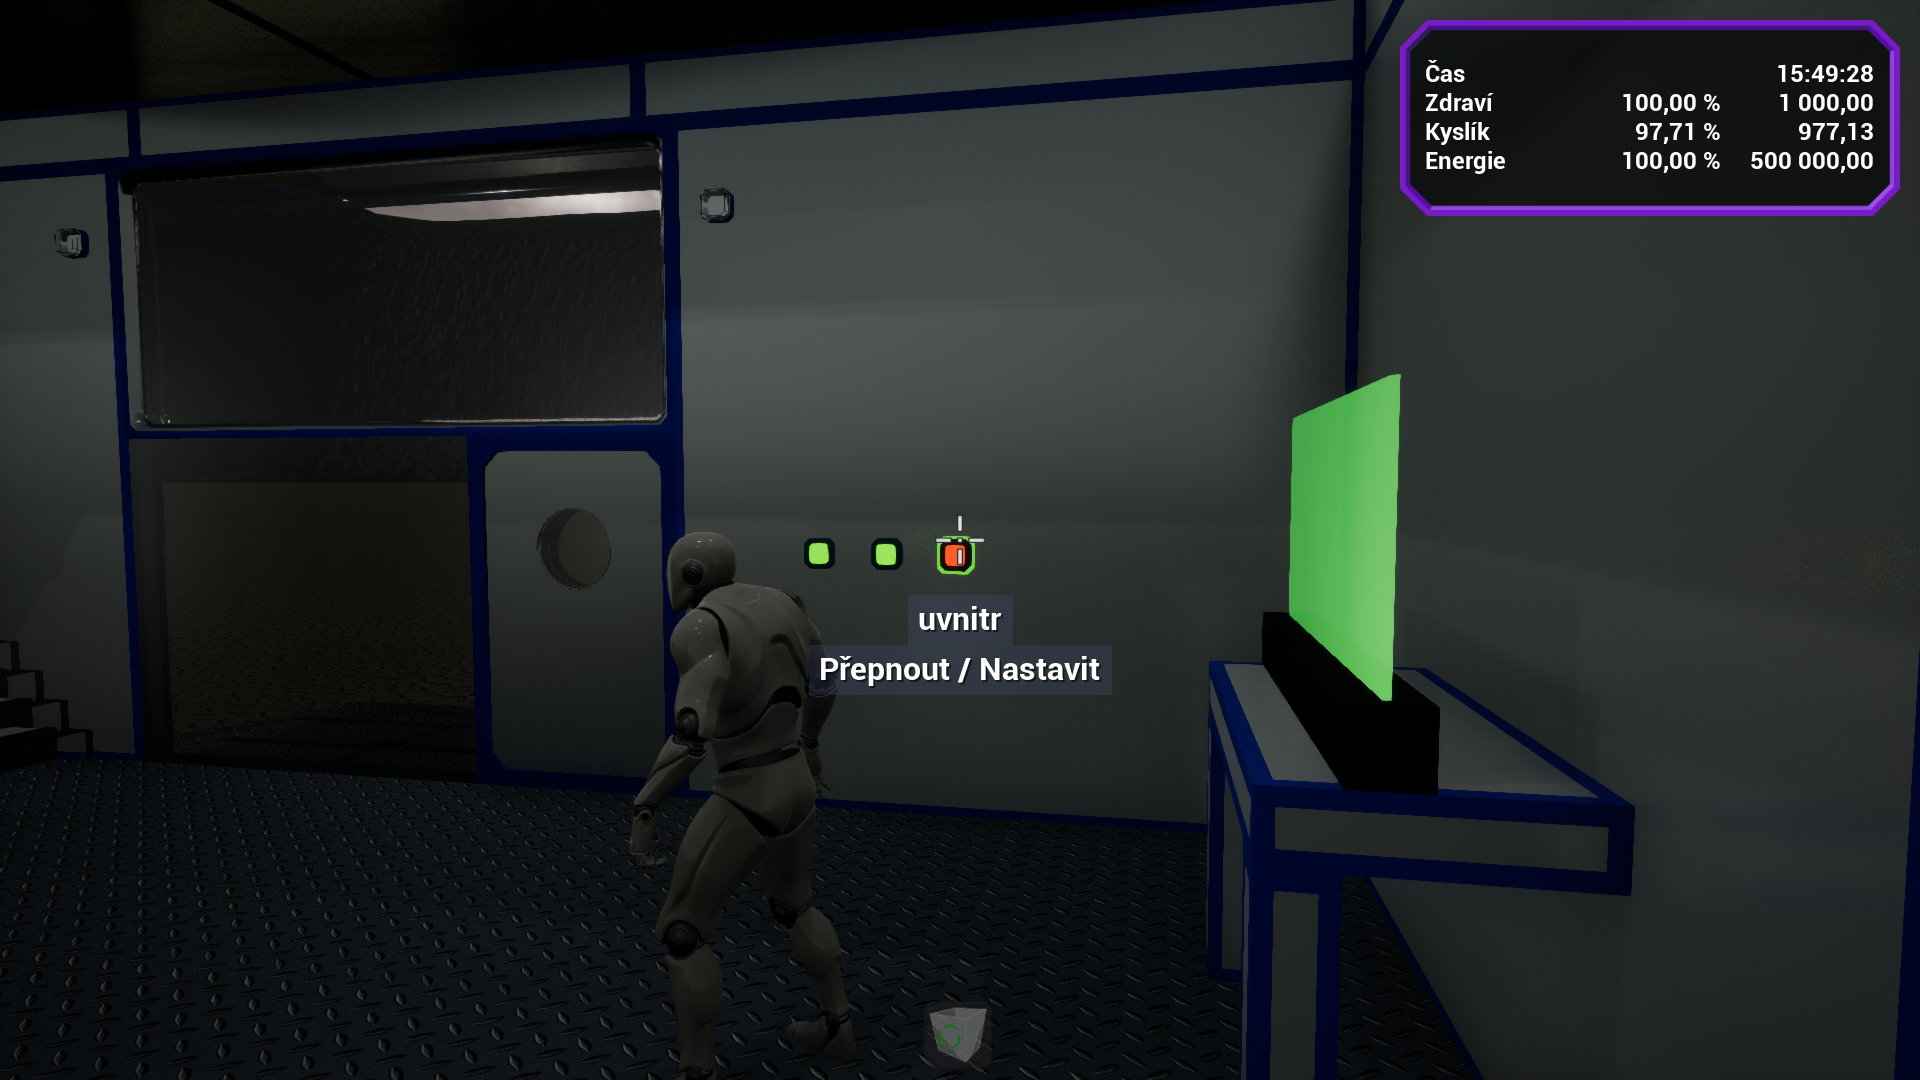
\includegraphics[ width=140mm]{../img/user/switcher/0switcherGeneral}

\caption{Přepínač - den}
\label{fig:user_switcher_0switcherGeneral}

\end{figure}

\FloatBarrier

Blok umožňuje reagovat na denní dobu - automatické přepínání na definovaný stav, pokud začne den, nebo začne noc.

V levé části le možné přiřazovat ovládané bloky

\begin{figure}[!h]\centering
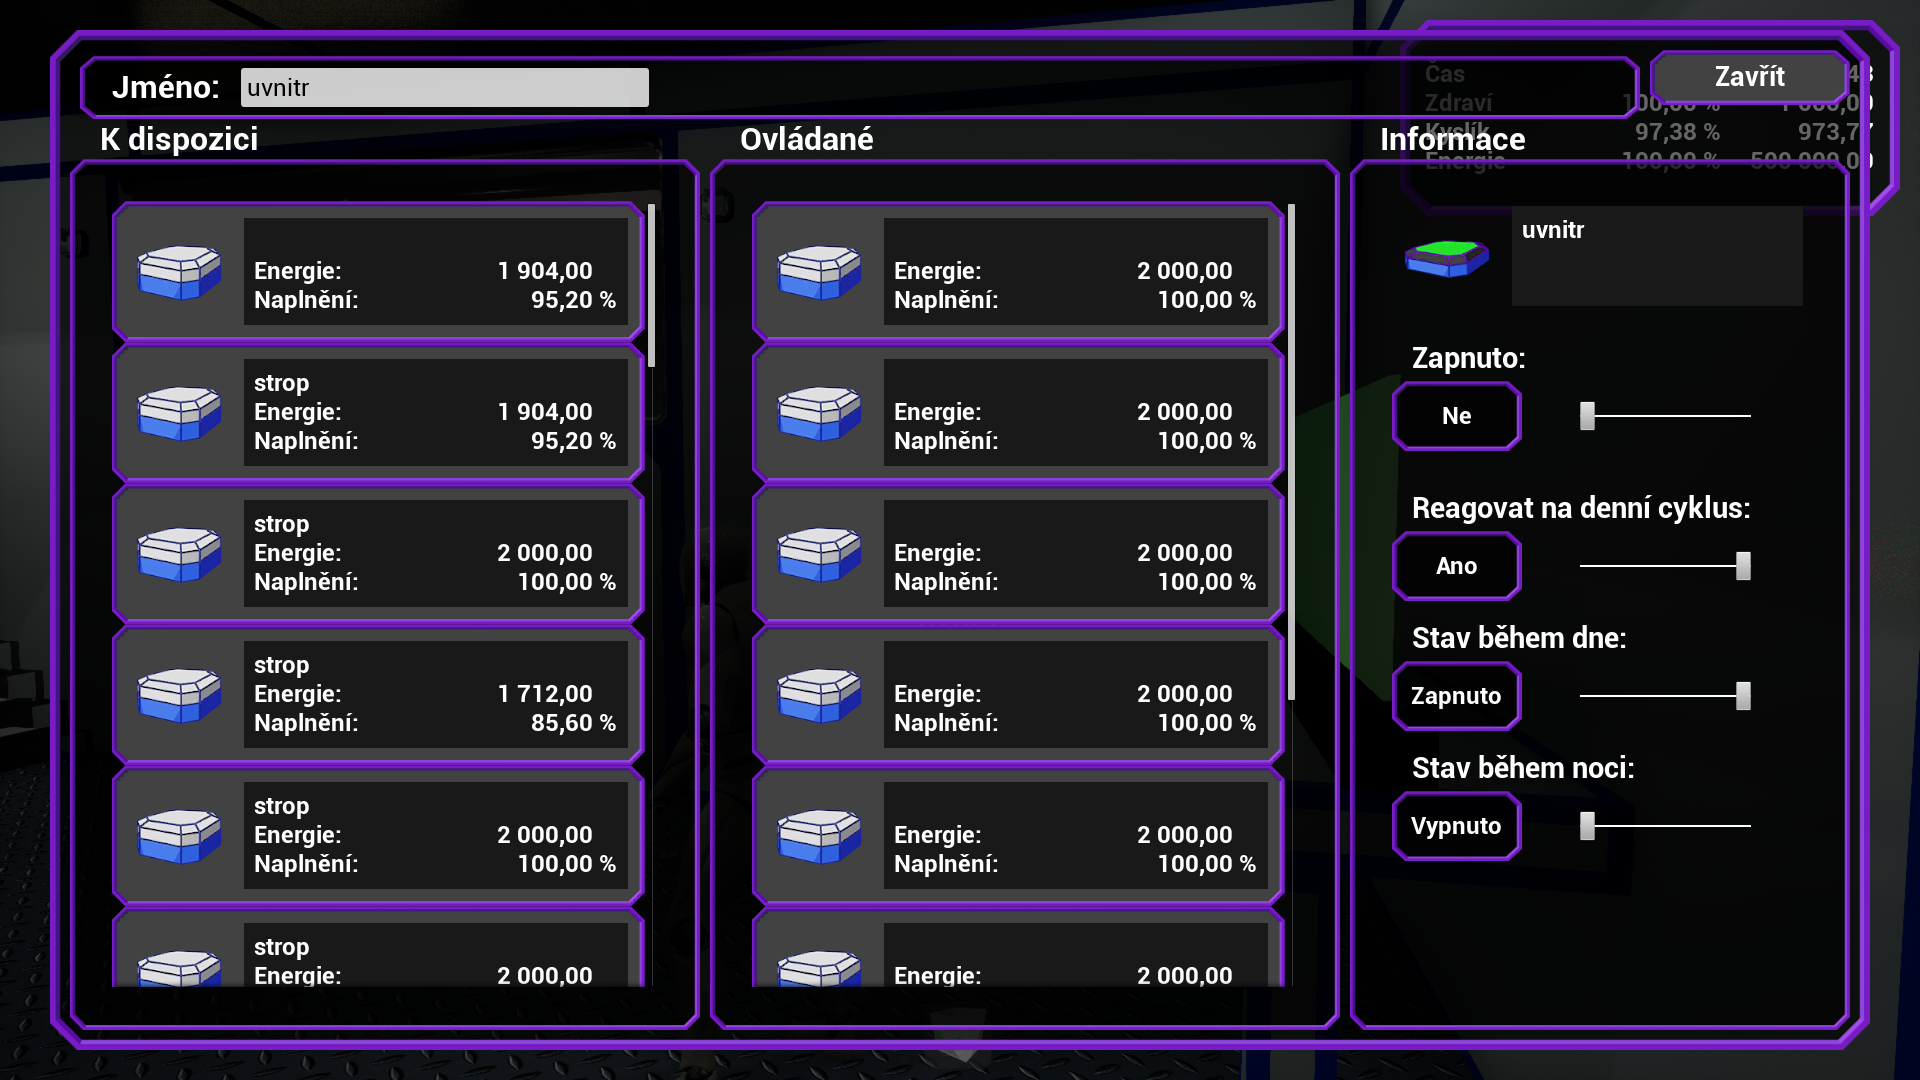
\includegraphics[ width=140mm]{../img/user/switcher/switcherControls}

\caption{Přepínač - poledne, zataženo}
\label{fig:user_switcher_switcherControls}

\end{figure}


\FloatBarrier
%%!TEX root = ../prace.tex

\section{Světlo}

Světlo má podobné rozhraní jako Plnička. V levé části se přiřazuje ovladač, v pravé se edituje výkon bloku.

\begin{figure}[!ht]\centering
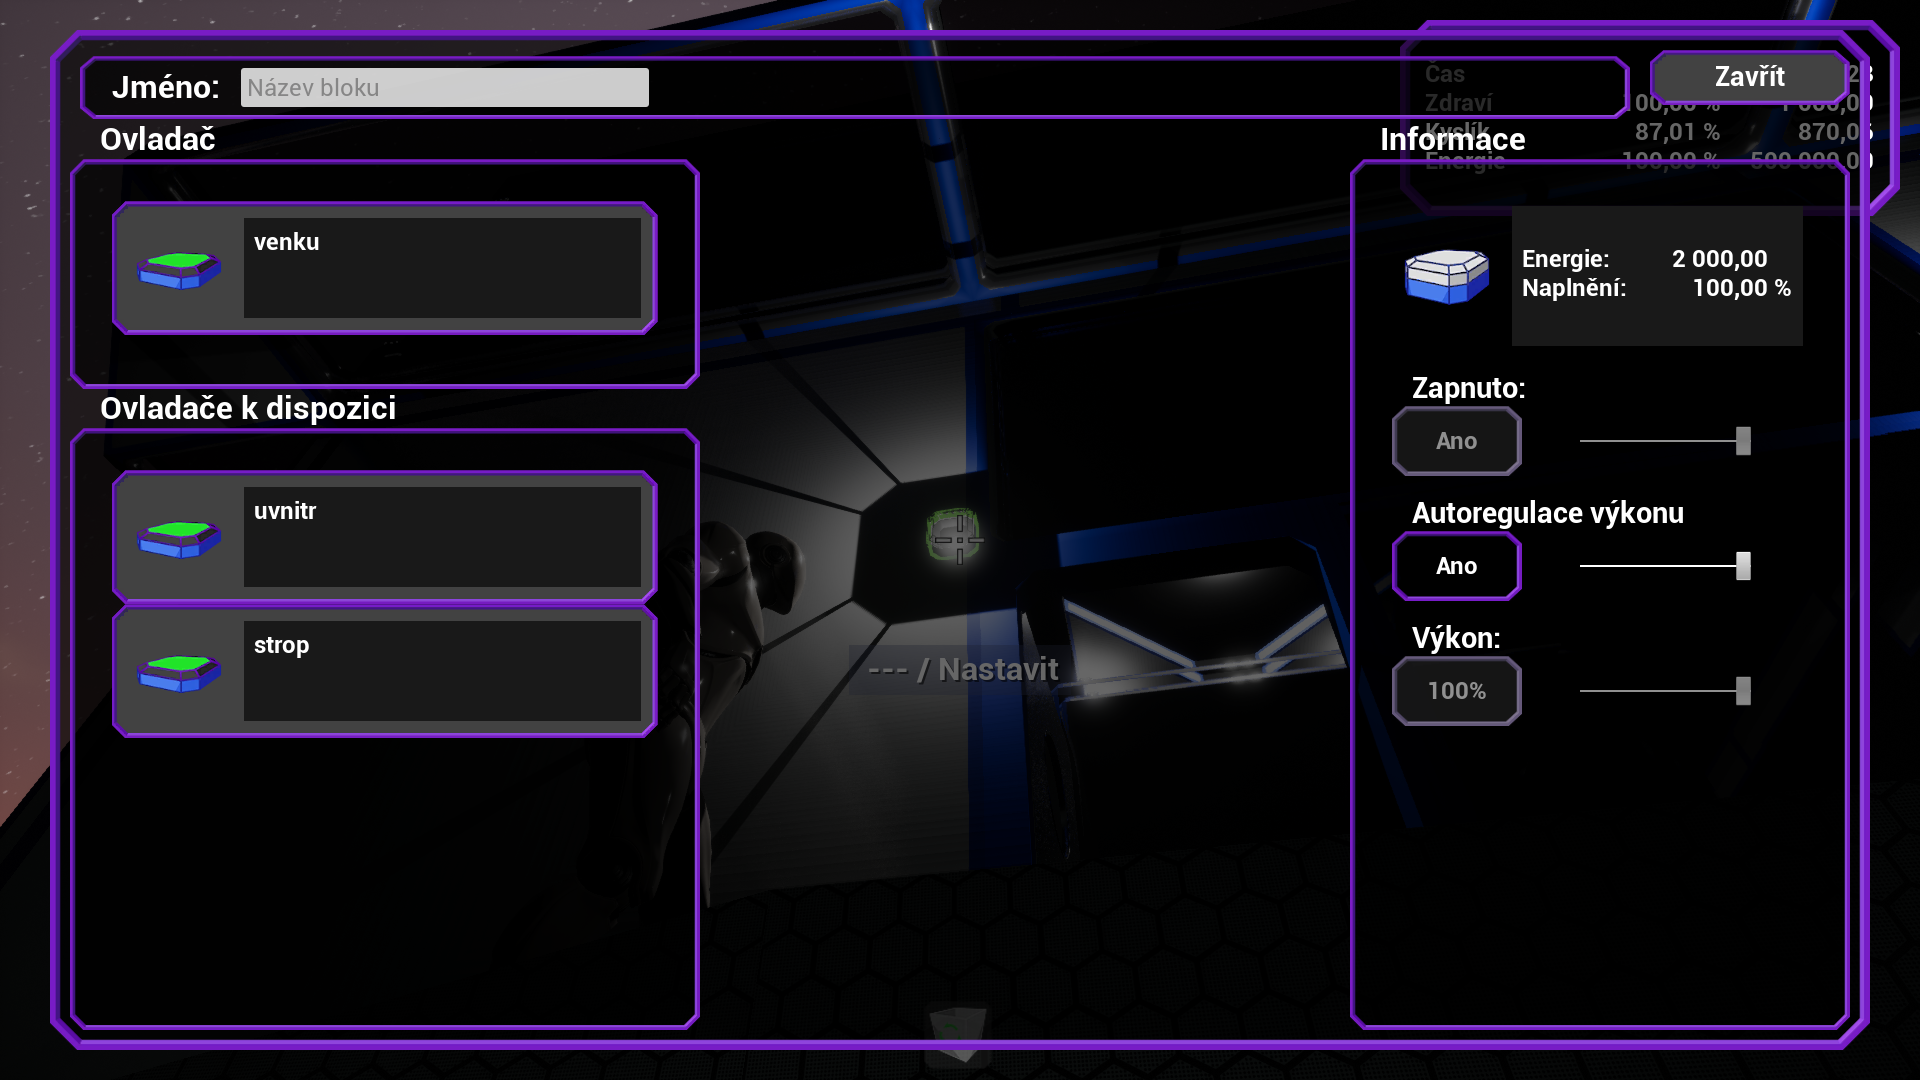
\includegraphics[ width=140mm]{../img/user/light/0light}

\caption{Světlo - ovládací obrazovka}
\label{fig:user_light_0light}

\end{figure}

\FloatBarrier

%%!TEX root = ../prace.tex

\section{Kyselý déšť}

Pokud se blíží bouře kyselého deště, nebo právě jedna probíhá, hráč vidí v levé horní části obrazovky zprávu s odhadovaným časem a intenzitou.

To umožňuje strategicky řídit chod svých budov a případně limitovat spotřebovávané zdroje v případě očekávaných dlouhotrvajících bouří. Odhadovaný čas je udán v herním čase.

\begin{figure}[!ht]\centering
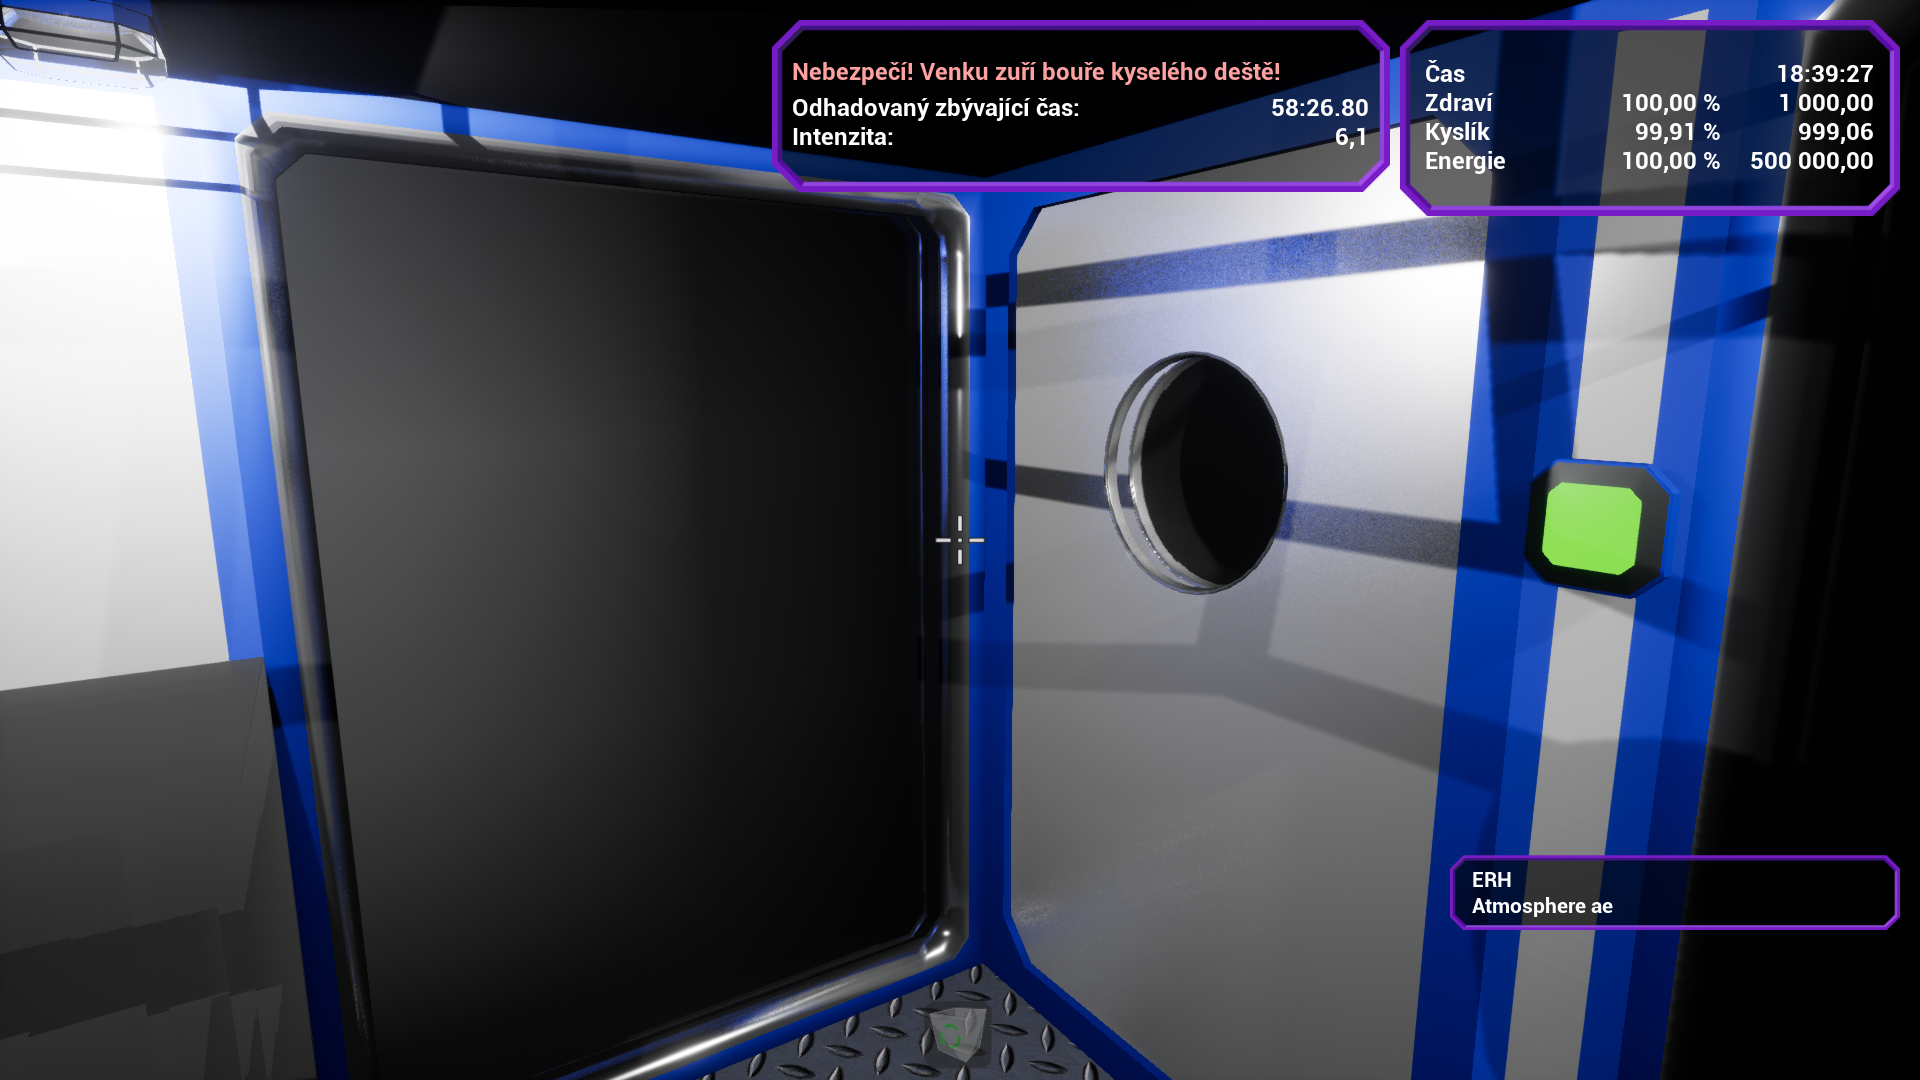
\includegraphics[ width=140mm]{../img/user/rain/0rainInfo}

\caption{Kyselý déšť - info}
\label{fig:user_rain_0rainInfo}

\end{figure}

\FloatBarrier

Pokud hráč není ukrytý v budově či pod nějakým blokem, dostává zásahy. Dokud má dostatek energie, je schopen odolávat účinkům bouře, v momentě, kdy mu energie dojde, začne mu ubývat zdraví.


\begin{figure}[!ht]\centering
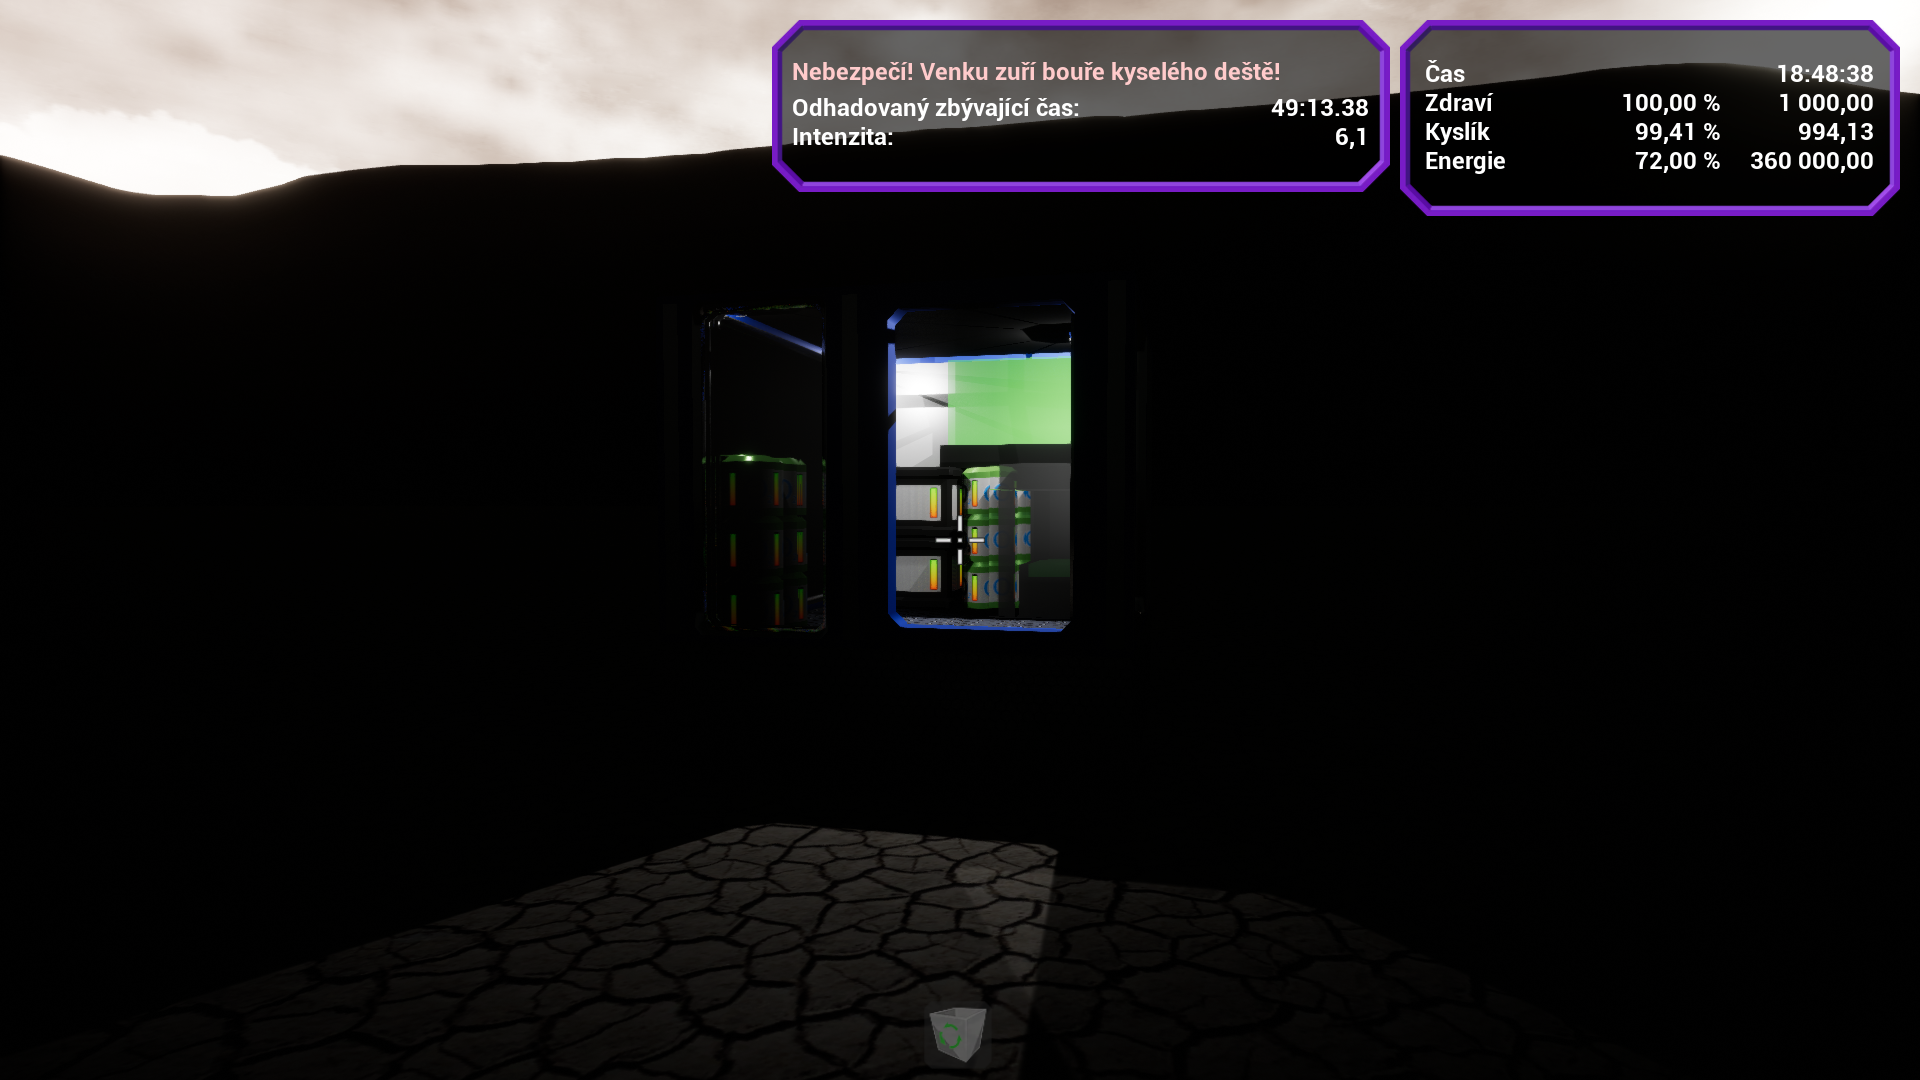
\includegraphics[ width=140mm]{../img/user/rain/1rainDamage}

\caption{Kyselý déšť - zásahy}
\label{fig:user_rain_1rainDamage}

\end{figure}

\FloatBarrier

Pokud si hráč doplní energii, začne se mu zdraví obnovovat.

\begin{figure}[!ht]\centering
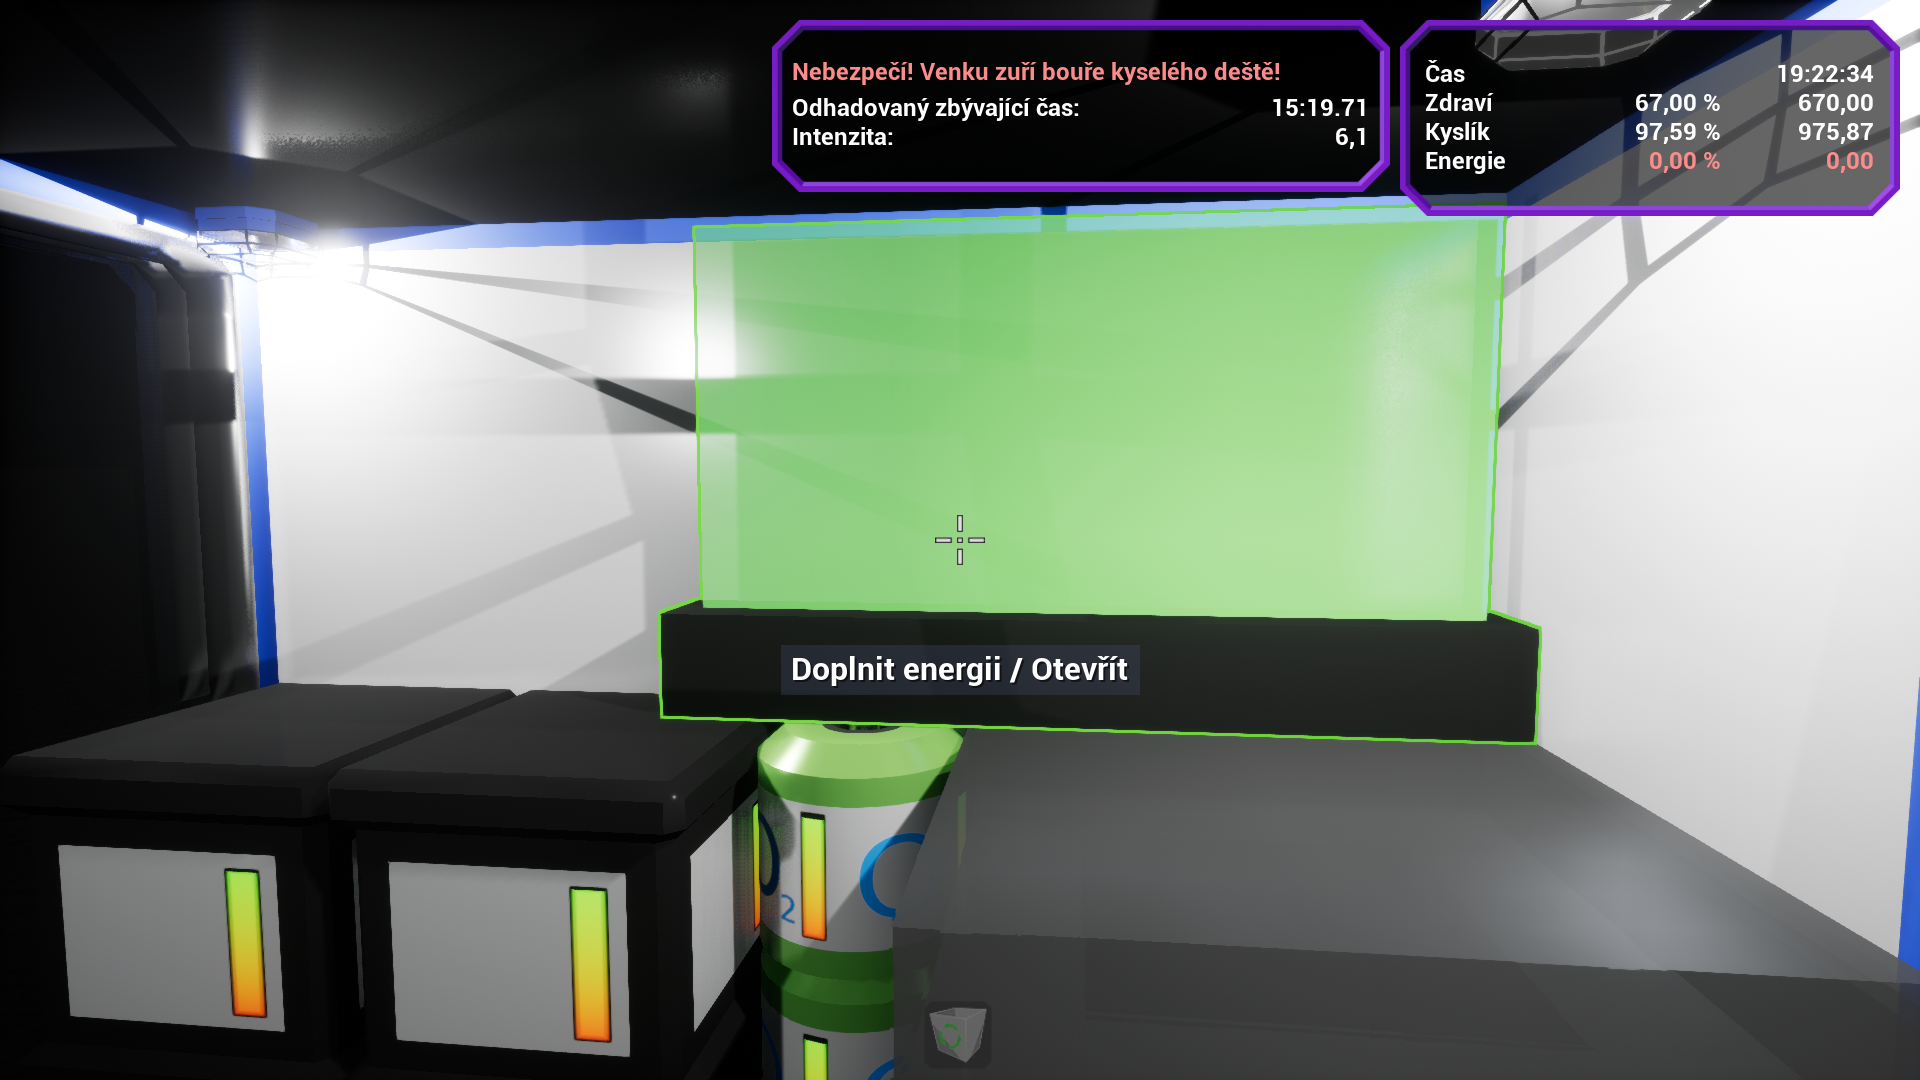
\includegraphics[ width=140mm]{../img/user/rain/2rainRefill}

\caption{Kyselý déšť - obnova zdraví}
\label{fig:user_rain_2rainRefill}

\end{figure}


\begin{figure}[!ht]\centering
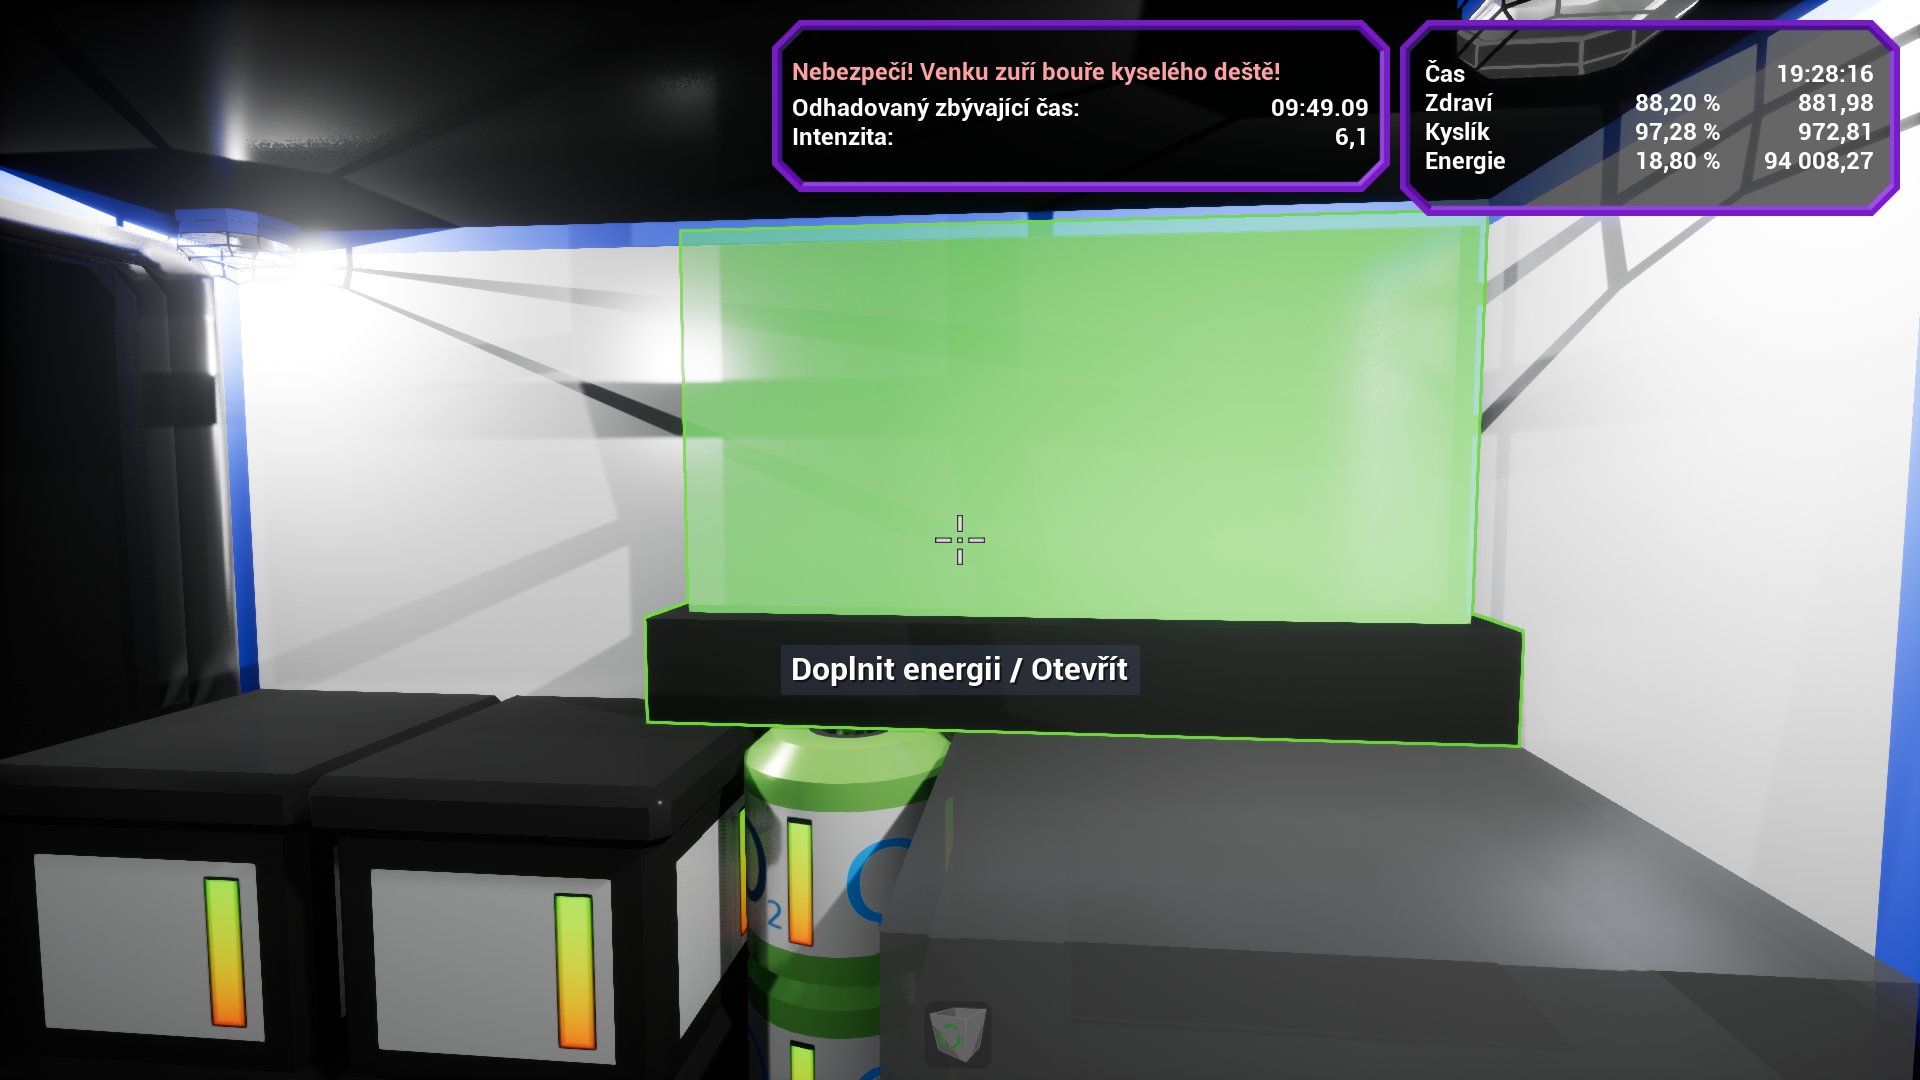
\includegraphics[ width=140mm]{../img/user/rain/3rainRefill1}

\caption{Kyselý déšť - obnova zdraví}
\label{fig:user_rain_3rainRefill1}

\end{figure}

\FloatBarrier

Během bouře je též možné pozorovat animaci generátoru energie, kdy je po každém zásahu rozsvícen příslušný čtverec. Tuto animaci lze z menu vypnout a pokud má uživatel slabší stroj, tak to i doporučujeme.

\begin{figure}[!ht]\centering
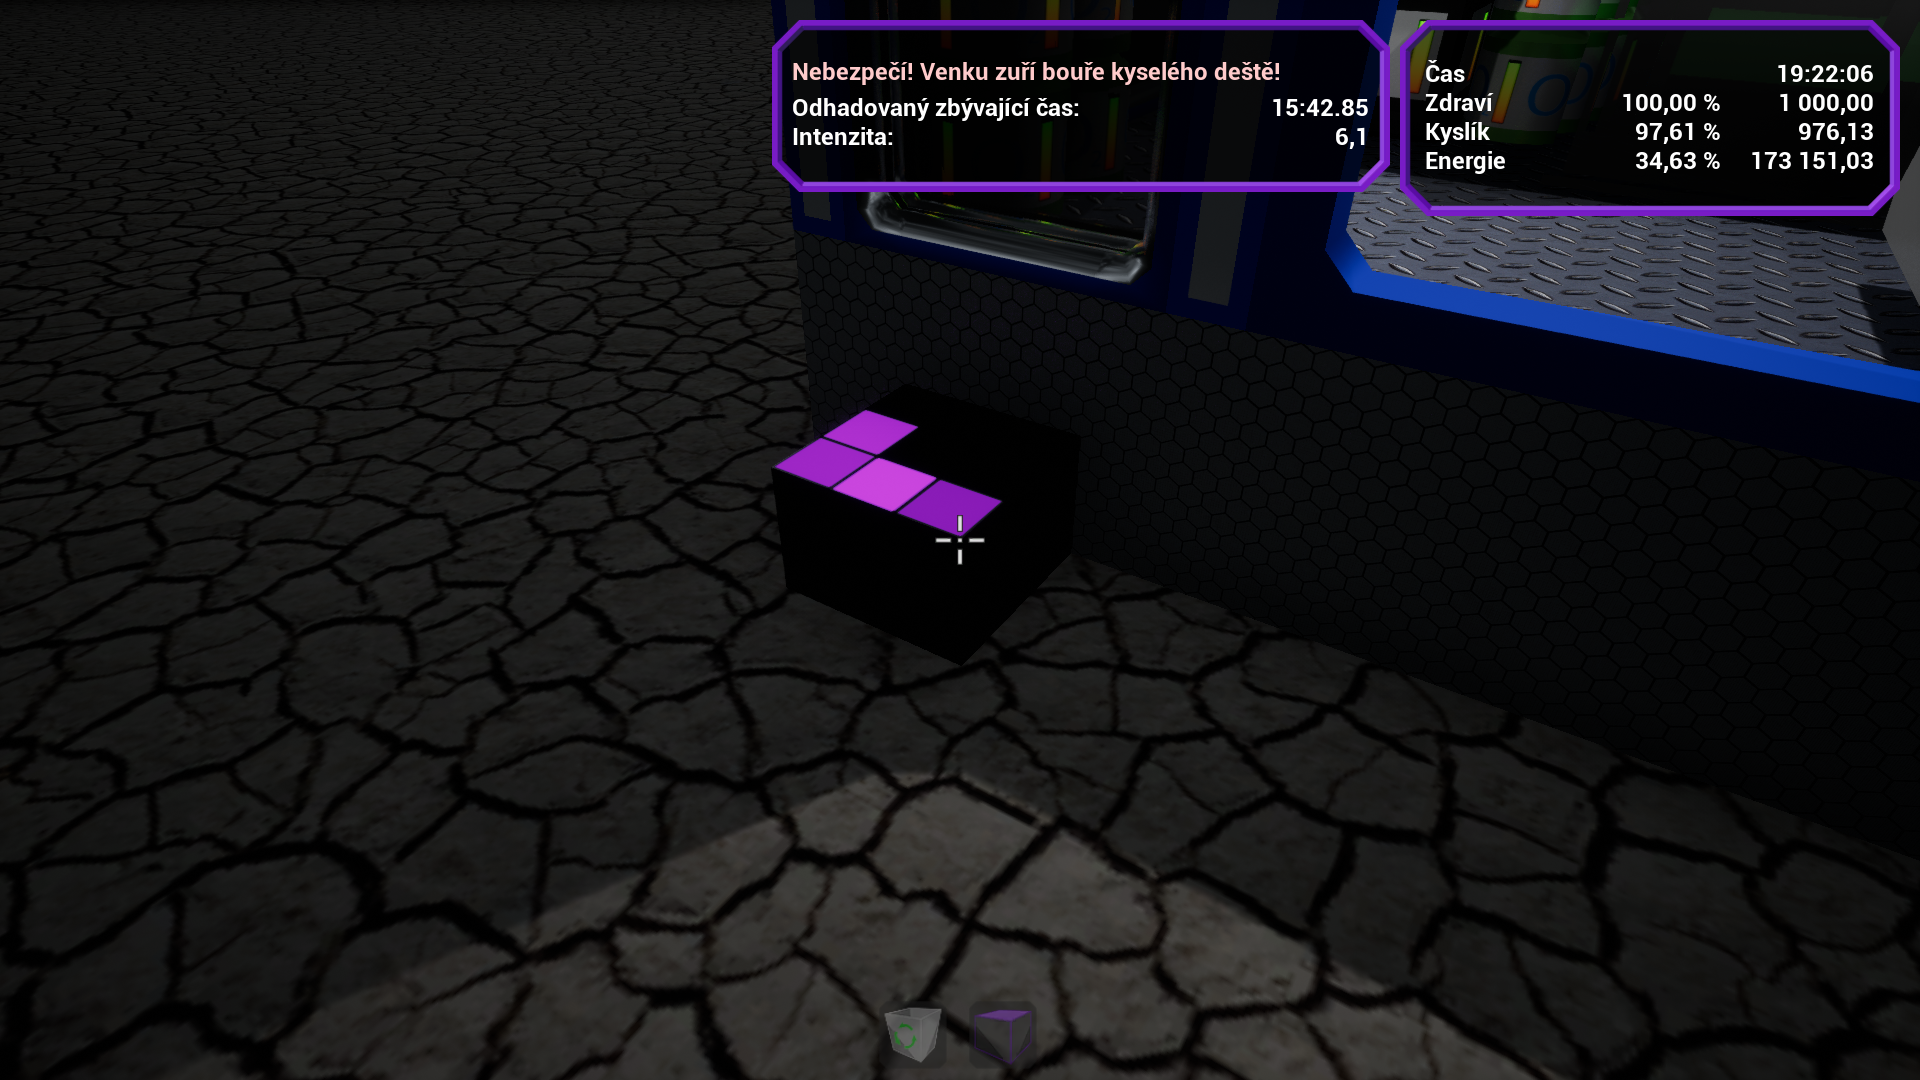
\includegraphics[ width=140mm]{../img/user/rain/4rainGeneratorAnim}

\caption{Kyselý déšť - animace zásahů}
\label{fig:user_rain_4rainGeneratorAnim}

\end{figure}


\FloatBarrier


